\subsubsection{Ausgewählte Untersuchungsgebiete für Referenzszenario aktualisierte Kostensätze (Nr. 4)}\label{chap_scenario_4_ausgewählte_untersuchungsgebiete}
Alle Untersuchungsgebiete, in denen Zügen der folgenden Kategorie(n) verkehren (siehe auch Abbildung \ref{fig_s_4_ausgewählte_untersuchungsgebiete}):
\begin{itemize}
    \item \acrlong{sgv}
\end{itemize}

Hinweis: Für Gebiete mit \acrshort{sgv} werden die Traktionsfälle Batterie und Wasserstoff nicht gerechnet.

\begin{center}
	\begin{figure}[p]
	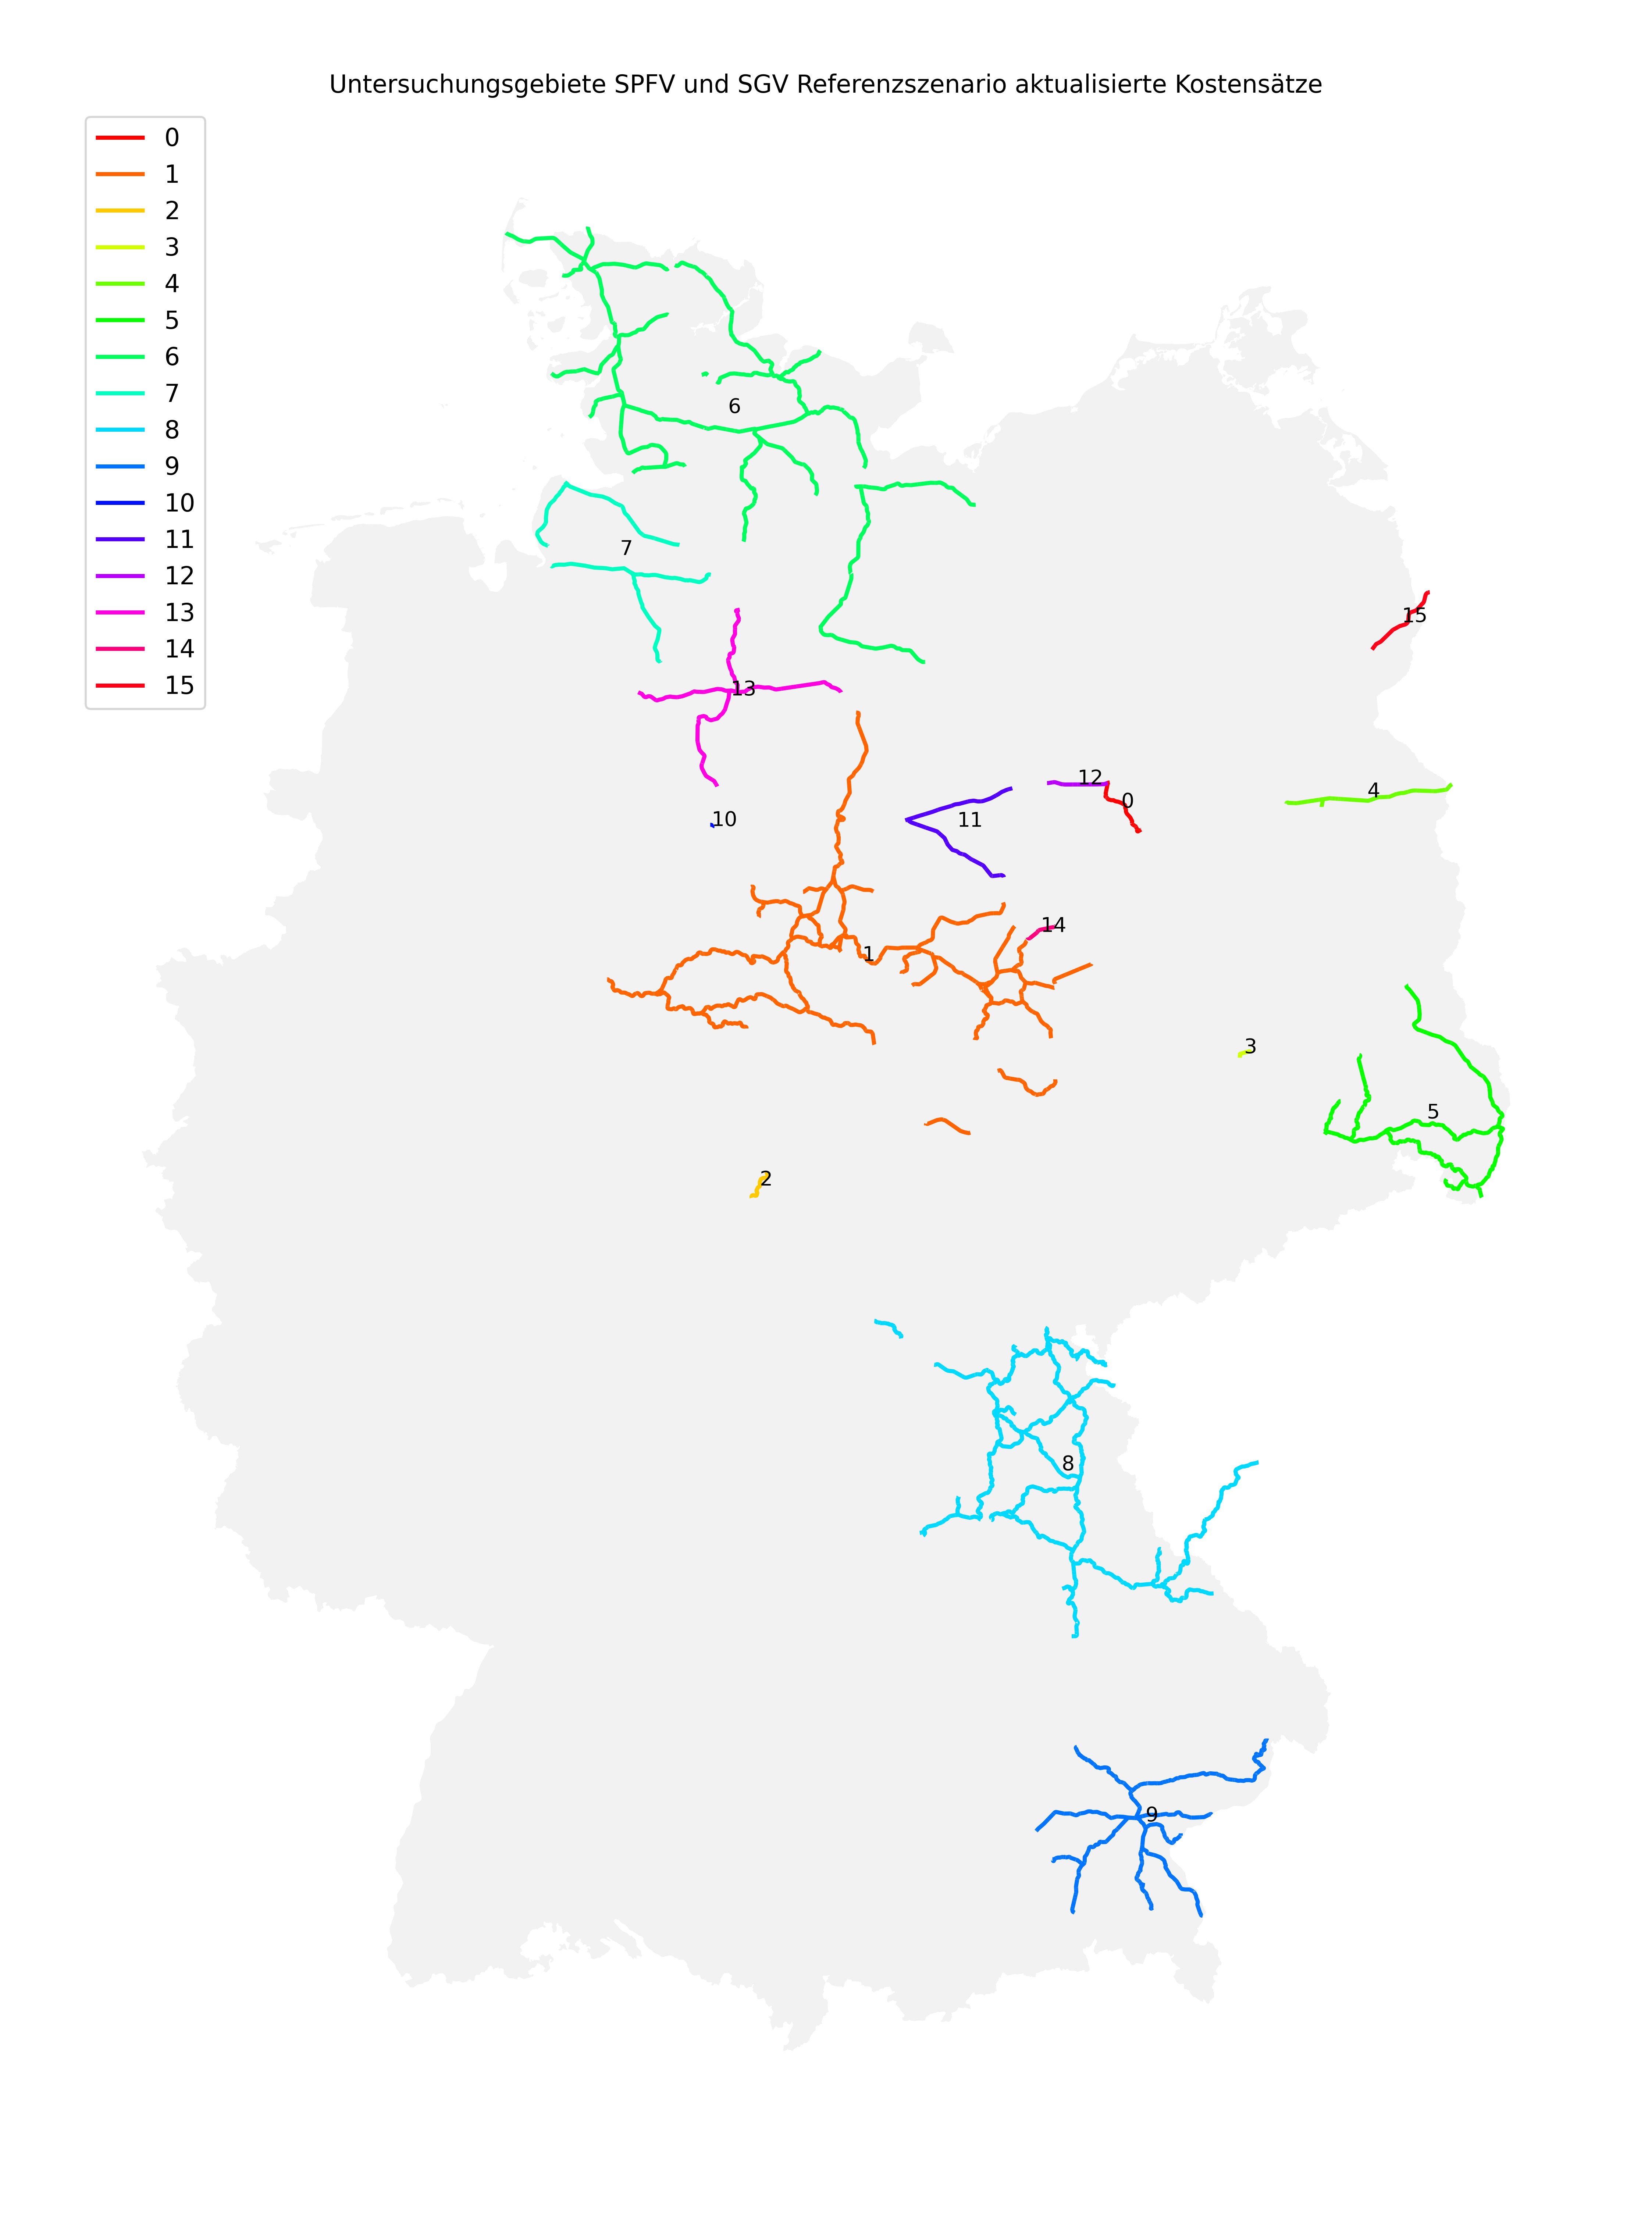
\includegraphics[height=0.85\textheight]{../report_scenarios/s_4/files/master_areas_sgv}
	\caption{\label{fig_s_4_ausgewählte_untersuchungsgebiete} Ausgewählte Untersuchungsgebiete für Szenario 4}
	\end{figure}
\end{center}


\begin{center}
\captionof{table}{\label{table_4_übersicht_untersuchungsgebiet_4} Übersicht ausgewählte Untersuchungsgebiete Szenrio 4}
\begin{tabularx}{\textwidth}{l | X | X | X | X} Nummer & kosteneffizienteste Traktion & Gesamtkosten kosteneffizienteste Traktion & Gesamtkosten e-Fuel & Gesamtkosten Diesel \\
\hline
0 &optimised electrification &
\SI{104046}{Tsd. \EUR} &
\SI{290288}{Tsd. \EUR} &
\SI{263339}{Tsd. \EUR} \\
1 &optimised electrification &
\SI{2383397}{Tsd. \EUR} &
\SI{4067278}{Tsd. \EUR} &
\SI{3999033}{Tsd. \EUR} \\
2 &electrification &
\SI{110916}{Tsd. \EUR} &
\SI{274835}{Tsd. \EUR} &
\SI{238453}{Tsd. \EUR} \\
3 &electrification &
\SI{46437}{Tsd. \EUR} &
\SI{112878}{Tsd. \EUR} &
\SI{98550}{Tsd. \EUR} \\
4 &optimised electrification &
\SI{310732}{Tsd. \EUR} &
\SI{569624}{Tsd. \EUR} &
\SI{556122}{Tsd. \EUR} \\
5 &optimised electrification &
\SI{1051137}{Tsd. \EUR} &
\SI{1870642}{Tsd. \EUR} &
\SI{1936918}{Tsd. \EUR} \\
6 &optimised electrification &
\SI{4156559}{Tsd. \EUR} &
\SI{10724074}{Tsd. \EUR} &
\SI{10178866}{Tsd. \EUR} \\
7 &optimised electrification &
\SI{917991}{Tsd. \EUR} &
\SI{2127587}{Tsd. \EUR} &
\SI{2015965}{Tsd. \EUR} \\
8 &optimised electrification &
\SI{4713641}{Tsd. \EUR} &
\SI{9477572}{Tsd. \EUR} &
\SI{9050737}{Tsd. \EUR} \\
9 &optimised electrification &
\SI{2638706}{Tsd. \EUR} &
\SI{7467403}{Tsd. \EUR} &
\SI{7046026}{Tsd. \EUR} \\
10 &electrification &
\SI{12430}{Tsd. \EUR} &
\SI{27962}{Tsd. \EUR} &
\SI{24848}{Tsd. \EUR} \\
11 &optimised electrification &
\SI{625987}{Tsd. \EUR} &
\SI{1802905}{Tsd. \EUR} &
\SI{1793453}{Tsd. \EUR} \\
12 &electrification &
\SI{327297}{Tsd. \EUR} &
\SI{918875}{Tsd. \EUR} &
\SI{898321}{Tsd. \EUR} \\
13 &optimised electrification &
\SI{779678}{Tsd. \EUR} &
\SI{1860553}{Tsd. \EUR} &
\SI{1708442}{Tsd. \EUR} \\
14 &electrification &
\SI{592562}{Tsd. \EUR} &
\SI{2248625}{Tsd. \EUR} &
\SI{2293446}{Tsd. \EUR} \\
15 &electrification &
\SI{487049}{Tsd. \EUR} &
\SI{1410691}{Tsd. \EUR} &
\SI{1384173}{Tsd. \EUR} \\
\end{tabularx}
\end{center}



	\paragraph*{Untersuchungsgebiet 0}\mbox{} \\
	\captionof{table}{\label{table_4_kenngrößen_untersuchungsgebiet_4607} Basiskenngrößen Untersuchungsgebiet 0}
	\begin{center}
		\begin{tabularx}{\textwidth}{X | r } Kenngröße & Wert \\
		\hline
		Länge & \SI{33.954}{\km} \\
		gewählte Traktion & optimised electrification \\
		Infrastrukturkosten gewählte Traktion (Barwert) & \SI{7483}{Tsd. \EUR} \\
		Betriebskosten gewählte Traktion (Barwert) & \SI{96563}{Tsd. \EUR}\\
		Gesamtkosten gewählte Traktion (Barwert) & \SI{104046}{Tsd. \EUR} \\
		\ce{CO2}-Jahresbilanz Ausgangssituation & \SI{9723}{\tonne} \ce{CO2} \\
		\ce{CO2}-Jahresbilanz Szenario & \SI{272}{\tonne} \ce{CO2} \\
		\end{tabularx}
	\end{center}

	\captionof{table}{\label{table_4_kosten_untersuchungsgebiet_4607} Kosten Untersuchungsgebiet verschiedene Traktionen 0}
	\begin{center}
		\begin{tabularx}{\textwidth}{X | X | X | X} Traktion & Infrastrukturkosten & Betriebskosten & Gesamtkosten\\
		\hline
									electrification & \SI{48670}{Tsd. \EUR} & \SI{87261}{Tsd. \EUR} & \SI{135931}{Tsd. \EUR}\\
												efuel & \SI{1556}{Tsd. \EUR} & \SI{288732}{Tsd. \EUR} & \SI{290288}{Tsd. \EUR}\\
																	optimised electrification & \SI{7483}{Tsd. \EUR} & \SI{96563}{Tsd. \EUR} & \SI{104046}{Tsd. \EUR}\\
												diesel & \SI{1556}{Tsd. \EUR} & \SI{261783}{Tsd. \EUR} & \SI{263339}{Tsd. \EUR}\\
												\end{tabularx}
	\end{center}
	\bigskip

		\captionof{table}{\label{tfig_4_betriebskosten_untersuchungsgebiet_4607_transportmode_} jährliche Betriebskosten Untersuchungsgebiet 0 für Zugkategorie \uppercase{sgv}}
	\begin{center}
		\begin{tabularx}{\textwidth}{X | X | X | X | X } Traktion & Gesamtkosten & Kapitaldienst & Instandhaltungs- kosten & Energiekosten\\
		\hline
					diesel &
			\SI{10677}{Tsd. \EUR} &
			\SI{1065}{Tsd. \EUR} &
			\SI{1089}{Tsd. \EUR} &
			\SI{2020}{Tsd. \EUR} \\
					efuel &
			\SI{12382}{Tsd. \EUR} &
			\SI{1065}{Tsd. \EUR} &
			\SI{1089}{Tsd. \EUR} &
			\SI{6738}{Tsd. \EUR} \\
					electrification &
			\SI{3649}{Tsd. \EUR} &
			\SI{887}{Tsd. \EUR} &
			\SI{543}{Tsd. \EUR} &
			\SI{1470}{Tsd. \EUR} \\
					optimised electrification &
			\SI{3649}{Tsd. \EUR} &
			\SI{887}{Tsd. \EUR} &
			\SI{543}{Tsd. \EUR} &
			\SI{1470}{Tsd. \EUR} \\
				\end{tabularx}
		\smallskip
		\begin{tabularx}{\textwidth}{X | X | X | X | X | X } Traktion &  \ce{CO2}-Kosten & Schadstoff- kosten & Primärenergie- kosten & THG-Emissionen Herstellung & CO2-Emissionen\\
		\hline
					diesel &
			\SI{5010}{Tsd. \EUR} &
			\SI{178}{Tsd. \EUR} &
			\SI{1315}{Tsd. \EUR} &
			\SI{0}{Tsd. \EUR} &
			\SI{7475}{\tonne} \ce{CO2} \\
					efuel &
			\SI{669}{Tsd. \EUR} &
			\SI{178}{Tsd. \EUR} &
			\SI{2646}{Tsd. \EUR} &
			\SI{0}{Tsd. \EUR} &
			\SI{998}{\tonne} \ce{CO2} \\
					electrification &
			\SI{147}{Tsd. \EUR} &
			\SI{4}{Tsd. \EUR} &
			\SI{594}{Tsd. \EUR} &
			\SI{0}{Tsd. \EUR} &
			\SI{222}{\tonne} \ce{CO2} \\
					optimised electrification &
			\SI{147}{Tsd. \EUR} &
			\SI{4}{Tsd. \EUR} &
			\SI{594}{Tsd. \EUR} &
			\SI{0}{Tsd. \EUR} &
			\SI{222}{\tonne} \ce{CO2} \\
				\end{tabularx}
		\medskip
	\end{center}
		\captionof{table}{\label{tfig_4_betriebskosten_untersuchungsgebiet_4607_transportmode_} jährliche Betriebskosten Untersuchungsgebiet 0 für Zugkategorie \uppercase{spnv}}
	\begin{center}
		\begin{tabularx}{\textwidth}{X | X | X | X | X } Traktion & Gesamtkosten & Kapitaldienst & Instandhaltungs- kosten & Energiekosten\\
		\hline
					battery &
			\SI{1500}{Tsd. \EUR} &
			\SI{352}{Tsd. \EUR} &
			\SI{636}{Tsd. \EUR} &
			\SI{328}{Tsd. \EUR} \\
					diesel &
			\SI{3282}{Tsd. \EUR} &
			\SI{282}{Tsd. \EUR} &
			\SI{428}{Tsd. \EUR} &
			\SI{608}{Tsd. \EUR} \\
					efuel &
			\SI{3014}{Tsd. \EUR} &
			\SI{282}{Tsd. \EUR} &
			\SI{428}{Tsd. \EUR} &
			\SI{1510}{Tsd. \EUR} \\
					electrification &
			\SI{1004}{Tsd. \EUR} &
			\SI{292}{Tsd. \EUR} &
			\SI{314}{Tsd. \EUR} &
			\SI{258}{Tsd. \EUR} \\
					h2 &
			\SI{1938}{Tsd. \EUR} &
			\SI{364}{Tsd. \EUR} &
			\SI{496}{Tsd. \EUR} &
			\SI{650}{Tsd. \EUR} \\
					optimised electrification &
			\SI{1500}{Tsd. \EUR} &
			\SI{352}{Tsd. \EUR} &
			\SI{636}{Tsd. \EUR} &
			\SI{328}{Tsd. \EUR} \\
				\end{tabularx}
		\smallskip
		\begin{tabularx}{\textwidth}{X | X | X | X | X | X } Traktion &  \ce{CO2}-Kosten & Schadstoff- kosten & Primärenergie- kosten & THG-Emissionen Herstellung & CO2-Emissionen\\
		\hline
					battery &
			\SI{34}{Tsd. \EUR} &
			\SI{2}{Tsd. \EUR} &
			\SI{132}{Tsd. \EUR} &
			\SI{16}{Tsd. \EUR} &
			\SI{50}{\tonne} \ce{CO2} \\
					diesel &
			\SI{1506}{Tsd. \EUR} &
			\SI{54}{Tsd. \EUR} &
			\SI{396}{Tsd. \EUR} &
			\SI{8}{Tsd. \EUR} &
			\SI{2248}{\tonne} \ce{CO2} \\
					efuel &
			\SI{150}{Tsd. \EUR} &
			\SI{40}{Tsd. \EUR} &
			\SI{594}{Tsd. \EUR} &
			\SI{8}{Tsd. \EUR} &
			\SI{224}{\tonne} \ce{CO2} \\
					electrification &
			\SI{26}{Tsd. \EUR} &
			\SI{0}{Tsd. \EUR} &
			\SI{104}{Tsd. \EUR} &
			\SI{10}{Tsd. \EUR} &
			\SI{38}{\tonne} \ce{CO2} \\
					h2 &
			\SI{82}{Tsd. \EUR} &
			\SI{2}{Tsd. \EUR} &
			\SI{324}{Tsd. \EUR} &
			\SI{20}{Tsd. \EUR} &
			\SI{122}{\tonne} \ce{CO2} \\
					optimised electrification &
			\SI{34}{Tsd. \EUR} &
			\SI{2}{Tsd. \EUR} &
			\SI{132}{Tsd. \EUR} &
			\SI{16}{Tsd. \EUR} &
			\SI{50}{\tonne} \ce{CO2} \\
				\end{tabularx}
		\medskip
	\end{center}
		\captionof{table}{\label{tfig_4_betriebskosten_untersuchungsgebiet_4607_transportmode_} jährliche Betriebskosten Untersuchungsgebiet 0 für Zugkategorie \uppercase{all}}
	\begin{center}
		\begin{tabularx}{\textwidth}{X | X | X | X | X } Traktion & Gesamtkosten & Kapitaldienst & Instandhaltungs- kosten & Energiekosten\\
		\hline
					battery &
			\SI{1500}{Tsd. \EUR} &
			\SI{352}{Tsd. \EUR} &
			\SI{636}{Tsd. \EUR} &
			\SI{328}{Tsd. \EUR} \\
					diesel &
			\SI{13959}{Tsd. \EUR} &
			\SI{1347}{Tsd. \EUR} &
			\SI{1517}{Tsd. \EUR} &
			\SI{2628}{Tsd. \EUR} \\
					efuel &
			\SI{15396}{Tsd. \EUR} &
			\SI{1347}{Tsd. \EUR} &
			\SI{1517}{Tsd. \EUR} &
			\SI{8248}{Tsd. \EUR} \\
					electrification &
			\SI{4653}{Tsd. \EUR} &
			\SI{1179}{Tsd. \EUR} &
			\SI{857}{Tsd. \EUR} &
			\SI{1728}{Tsd. \EUR} \\
					h2 &
			\SI{1938}{Tsd. \EUR} &
			\SI{364}{Tsd. \EUR} &
			\SI{496}{Tsd. \EUR} &
			\SI{650}{Tsd. \EUR} \\
					optimised electrification &
			\SI{5149}{Tsd. \EUR} &
			\SI{1239}{Tsd. \EUR} &
			\SI{1179}{Tsd. \EUR} &
			\SI{1798}{Tsd. \EUR} \\
				\end{tabularx}
		\smallskip
		\begin{tabularx}{\textwidth}{X | X | X | X | X | X } Traktion &  \ce{CO2}-Kosten & Schadstoff- kosten & Primärenergie- kosten & THG-Emissionen Herstellung & CO2-Emissionen\\
		\hline
					battery &
			\SI{34}{Tsd. \EUR} &
			\SI{2}{Tsd. \EUR} &
			\SI{132}{Tsd. \EUR} &
			\SI{16}{Tsd. \EUR} &
			\SI{50}{\tonne} \ce{CO2} \\
					diesel &
			\SI{6516}{Tsd. \EUR} &
			\SI{232}{Tsd. \EUR} &
			\SI{1711}{Tsd. \EUR} &
			\SI{8}{Tsd. \EUR} &
			\SI{9723}{\tonne} \ce{CO2} \\
					efuel &
			\SI{819}{Tsd. \EUR} &
			\SI{218}{Tsd. \EUR} &
			\SI{3240}{Tsd. \EUR} &
			\SI{8}{Tsd. \EUR} &
			\SI{1222}{\tonne} \ce{CO2} \\
					electrification &
			\SI{173}{Tsd. \EUR} &
			\SI{4}{Tsd. \EUR} &
			\SI{698}{Tsd. \EUR} &
			\SI{10}{Tsd. \EUR} &
			\SI{260}{\tonne} \ce{CO2} \\
					h2 &
			\SI{82}{Tsd. \EUR} &
			\SI{2}{Tsd. \EUR} &
			\SI{324}{Tsd. \EUR} &
			\SI{20}{Tsd. \EUR} &
			\SI{122}{\tonne} \ce{CO2} \\
					optimised electrification &
			\SI{181}{Tsd. \EUR} &
			\SI{6}{Tsd. \EUR} &
			\SI{726}{Tsd. \EUR} &
			\SI{16}{Tsd. \EUR} &
			\SI{272}{\tonne} \ce{CO2} \\
				\end{tabularx}
		\medskip
	\end{center}
	
\textit{Untersuchungsgebiet ID in Datenbank 4607}
	\paragraph*{Untersuchungsgebiet 1}\mbox{} \\
	\captionof{table}{\label{table_4_kenngrößen_untersuchungsgebiet_4589} Basiskenngrößen Untersuchungsgebiet 1}
	\begin{center}
		\begin{tabularx}{\textwidth}{X | r } Kenngröße & Wert \\
		\hline
		Länge & \SI{1049.579}{\km} \\
		gewählte Traktion & optimised electrification \\
		Infrastrukturkosten gewählte Traktion (Barwert) & \SI{617736}{Tsd. \EUR} \\
		Betriebskosten gewählte Traktion (Barwert) & \SI{1765661}{Tsd. \EUR}\\
		Gesamtkosten gewählte Traktion (Barwert) & \SI{2383397}{Tsd. \EUR} \\
		\ce{CO2}-Jahresbilanz Ausgangssituation & \SI{139646}{\tonne} \ce{CO2} \\
		\ce{CO2}-Jahresbilanz Szenario & \SI{3478}{\tonne} \ce{CO2} \\
		\end{tabularx}
	\end{center}

	\captionof{table}{\label{table_4_kosten_untersuchungsgebiet_4589} Kosten Untersuchungsgebiet verschiedene Traktionen 1}
	\begin{center}
		\begin{tabularx}{\textwidth}{X | X | X | X} Traktion & Infrastrukturkosten & Betriebskosten & Gesamtkosten\\
		\hline
									electrification & \SI{1968097}{Tsd. \EUR} & \SI{1368983}{Tsd. \EUR} & \SI{3337080}{Tsd. \EUR}\\
												efuel & \SI{42021}{Tsd. \EUR} & \SI{4025257}{Tsd. \EUR} & \SI{4067278}{Tsd. \EUR}\\
																	optimised electrification & \SI{617736}{Tsd. \EUR} & \SI{1765661}{Tsd. \EUR} & \SI{2383397}{Tsd. \EUR}\\
												diesel & \SI{42021}{Tsd. \EUR} & \SI{3957012}{Tsd. \EUR} & \SI{3999033}{Tsd. \EUR}\\
												\end{tabularx}
	\end{center}
	\bigskip

		\captionof{table}{\label{tfig_4_betriebskosten_untersuchungsgebiet_4589_transportmode_} jährliche Betriebskosten Untersuchungsgebiet 1 für Zugkategorie \uppercase{sgv}}
	\begin{center}
		\begin{tabularx}{\textwidth}{X | X | X | X | X } Traktion & Gesamtkosten & Kapitaldienst & Instandhaltungs- kosten & Energiekosten\\
		\hline
					diesel &
			\SI{45803}{Tsd. \EUR} &
			\SI{6010}{Tsd. \EUR} &
			\SI{4504}{Tsd. \EUR} &
			\SI{8368}{Tsd. \EUR} \\
					efuel &
			\SI{52862}{Tsd. \EUR} &
			\SI{6010}{Tsd. \EUR} &
			\SI{4504}{Tsd. \EUR} &
			\SI{27892}{Tsd. \EUR} \\
					electrification &
			\SI{16440}{Tsd. \EUR} &
			\SI{5005}{Tsd. \EUR} &
			\SI{2248}{Tsd. \EUR} &
			\SI{6088}{Tsd. \EUR} \\
					optimised electrification &
			\SI{16440}{Tsd. \EUR} &
			\SI{5005}{Tsd. \EUR} &
			\SI{2248}{Tsd. \EUR} &
			\SI{6088}{Tsd. \EUR} \\
				\end{tabularx}
		\smallskip
		\begin{tabularx}{\textwidth}{X | X | X | X | X | X } Traktion &  \ce{CO2}-Kosten & Schadstoff- kosten & Primärenergie- kosten & THG-Emissionen Herstellung & CO2-Emissionen\\
		\hline
					diesel &
			\SI{20742}{Tsd. \EUR} &
			\SI{732}{Tsd. \EUR} &
			\SI{5450}{Tsd. \EUR} &
			\SI{0}{Tsd. \EUR} &
			\SI{30952}{\tonne} \ce{CO2} \\
					efuel &
			\SI{2764}{Tsd. \EUR} &
			\SI{732}{Tsd. \EUR} &
			\SI{10956}{Tsd. \EUR} &
			\SI{0}{Tsd. \EUR} &
			\SI{4126}{\tonne} \ce{CO2} \\
					electrification &
			\SI{612}{Tsd. \EUR} &
			\SI{22}{Tsd. \EUR} &
			\SI{2458}{Tsd. \EUR} &
			\SI{0}{Tsd. \EUR} &
			\SI{912}{\tonne} \ce{CO2} \\
					optimised electrification &
			\SI{612}{Tsd. \EUR} &
			\SI{22}{Tsd. \EUR} &
			\SI{2458}{Tsd. \EUR} &
			\SI{0}{Tsd. \EUR} &
			\SI{912}{\tonne} \ce{CO2} \\
				\end{tabularx}
		\medskip
	\end{center}
		\captionof{table}{\label{tfig_4_betriebskosten_untersuchungsgebiet_4589_transportmode_} jährliche Betriebskosten Untersuchungsgebiet 1 für Zugkategorie \uppercase{spnv}}
	\begin{center}
		\begin{tabularx}{\textwidth}{X | X | X | X | X } Traktion & Gesamtkosten & Kapitaldienst & Instandhaltungs- kosten & Energiekosten\\
		\hline
					efuel &
			\SI{161776}{Tsd. \EUR} &
			\SI{15532}{Tsd. \EUR} &
			\SI{25248}{Tsd. \EUR} &
			\SI{79380}{Tsd. \EUR} \\
					h2 &
			\SI{108756}{Tsd. \EUR} &
			\SI{19946}{Tsd. \EUR} &
			\SI{29284}{Tsd. \EUR} &
			\SI{35870}{Tsd. \EUR} \\
					battery &
			\SI{83472}{Tsd. \EUR} &
			\SI{19316}{Tsd. \EUR} &
			\SI{36316}{Tsd. \EUR} &
			\SI{17884}{Tsd. \EUR} \\
					electrification &
			\SI{56558}{Tsd. \EUR} &
			\SI{15980}{Tsd. \EUR} &
			\SI{18504}{Tsd. \EUR} &
			\SI{14302}{Tsd. \EUR} \\
					diesel &
			\SI{165196}{Tsd. \EUR} &
			\SI{15532}{Tsd. \EUR} &
			\SI{25248}{Tsd. \EUR} &
			\SI{29388}{Tsd. \EUR} \\
					optimised electrification &
			\SI{77710}{Tsd. \EUR} &
			\SI{18532}{Tsd. \EUR} &
			\SI{32570}{Tsd. \EUR} &
			\SI{17122}{Tsd. \EUR} \\
				\end{tabularx}
		\smallskip
		\begin{tabularx}{\textwidth}{X | X | X | X | X | X } Traktion &  \ce{CO2}-Kosten & Schadstoff- kosten & Primärenergie- kosten & THG-Emissionen Herstellung & CO2-Emissionen\\
		\hline
					efuel &
			\SI{7866}{Tsd. \EUR} &
			\SI{2080}{Tsd. \EUR} &
			\SI{31176}{Tsd. \EUR} &
			\SI{484}{Tsd. \EUR} &
			\SI{11748}{\tonne} \ce{CO2} \\
					h2 &
			\SI{4516}{Tsd. \EUR} &
			\SI{154}{Tsd. \EUR} &
			\SI{17894}{Tsd. \EUR} &
			\SI{1078}{Tsd. \EUR} &
			\SI{6728}{\tonne} \ce{CO2} \\
					battery &
			\SI{1796}{Tsd. \EUR} &
			\SI{60}{Tsd. \EUR} &
			\SI{7216}{Tsd. \EUR} &
			\SI{884}{Tsd. \EUR} &
			\SI{2682}{\tonne} \ce{CO2} \\
					electrification &
			\SI{1434}{Tsd. \EUR} &
			\SI{48}{Tsd. \EUR} &
			\SI{5770}{Tsd. \EUR} &
			\SI{518}{Tsd. \EUR} &
			\SI{2144}{\tonne} \ce{CO2} \\
					diesel &
			\SI{72828}{Tsd. \EUR} &
			\SI{2578}{Tsd. \EUR} &
			\SI{19136}{Tsd. \EUR} &
			\SI{484}{Tsd. \EUR} &
			\SI{108694}{\tonne} \ce{CO2} \\
					optimised electrification &
			\SI{1718}{Tsd. \EUR} &
			\SI{58}{Tsd. \EUR} &
			\SI{6910}{Tsd. \EUR} &
			\SI{796}{Tsd. \EUR} &
			\SI{2566}{\tonne} \ce{CO2} \\
				\end{tabularx}
		\medskip
	\end{center}
		\captionof{table}{\label{tfig_4_betriebskosten_untersuchungsgebiet_4589_transportmode_} jährliche Betriebskosten Untersuchungsgebiet 1 für Zugkategorie \uppercase{all}}
	\begin{center}
		\begin{tabularx}{\textwidth}{X | X | X | X | X } Traktion & Gesamtkosten & Kapitaldienst & Instandhaltungs- kosten & Energiekosten\\
		\hline
					efuel &
			\SI{214638}{Tsd. \EUR} &
			\SI{21542}{Tsd. \EUR} &
			\SI{29752}{Tsd. \EUR} &
			\SI{107272}{Tsd. \EUR} \\
					h2 &
			\SI{108756}{Tsd. \EUR} &
			\SI{19946}{Tsd. \EUR} &
			\SI{29284}{Tsd. \EUR} &
			\SI{35870}{Tsd. \EUR} \\
					battery &
			\SI{83472}{Tsd. \EUR} &
			\SI{19316}{Tsd. \EUR} &
			\SI{36316}{Tsd. \EUR} &
			\SI{17884}{Tsd. \EUR} \\
					electrification &
			\SI{72998}{Tsd. \EUR} &
			\SI{20985}{Tsd. \EUR} &
			\SI{20752}{Tsd. \EUR} &
			\SI{20390}{Tsd. \EUR} \\
					diesel &
			\SI{210999}{Tsd. \EUR} &
			\SI{21542}{Tsd. \EUR} &
			\SI{29752}{Tsd. \EUR} &
			\SI{37756}{Tsd. \EUR} \\
					optimised electrification &
			\SI{94150}{Tsd. \EUR} &
			\SI{23537}{Tsd. \EUR} &
			\SI{34818}{Tsd. \EUR} &
			\SI{23210}{Tsd. \EUR} \\
				\end{tabularx}
		\smallskip
		\begin{tabularx}{\textwidth}{X | X | X | X | X | X } Traktion &  \ce{CO2}-Kosten & Schadstoff- kosten & Primärenergie- kosten & THG-Emissionen Herstellung & CO2-Emissionen\\
		\hline
					efuel &
			\SI{10630}{Tsd. \EUR} &
			\SI{2812}{Tsd. \EUR} &
			\SI{42132}{Tsd. \EUR} &
			\SI{484}{Tsd. \EUR} &
			\SI{15874}{\tonne} \ce{CO2} \\
					h2 &
			\SI{4516}{Tsd. \EUR} &
			\SI{154}{Tsd. \EUR} &
			\SI{17894}{Tsd. \EUR} &
			\SI{1078}{Tsd. \EUR} &
			\SI{6728}{\tonne} \ce{CO2} \\
					battery &
			\SI{1796}{Tsd. \EUR} &
			\SI{60}{Tsd. \EUR} &
			\SI{7216}{Tsd. \EUR} &
			\SI{884}{Tsd. \EUR} &
			\SI{2682}{\tonne} \ce{CO2} \\
					electrification &
			\SI{2046}{Tsd. \EUR} &
			\SI{70}{Tsd. \EUR} &
			\SI{8228}{Tsd. \EUR} &
			\SI{518}{Tsd. \EUR} &
			\SI{3056}{\tonne} \ce{CO2} \\
					diesel &
			\SI{93570}{Tsd. \EUR} &
			\SI{3310}{Tsd. \EUR} &
			\SI{24586}{Tsd. \EUR} &
			\SI{484}{Tsd. \EUR} &
			\SI{139646}{\tonne} \ce{CO2} \\
					optimised electrification &
			\SI{2330}{Tsd. \EUR} &
			\SI{80}{Tsd. \EUR} &
			\SI{9368}{Tsd. \EUR} &
			\SI{796}{Tsd. \EUR} &
			\SI{3478}{\tonne} \ce{CO2} \\
				\end{tabularx}
		\medskip
	\end{center}
	
\textit{Untersuchungsgebiet ID in Datenbank 4589}
	\paragraph*{Untersuchungsgebiet 2}\mbox{} \\
	\captionof{table}{\label{table_4_kenngrößen_untersuchungsgebiet_4608} Basiskenngrößen Untersuchungsgebiet 2}
	\begin{center}
		\begin{tabularx}{\textwidth}{X | r } Kenngröße & Wert \\
		\hline
		Länge & \SI{17.785}{\km} \\
		gewählte Traktion & electrification \\
		Infrastrukturkosten gewählte Traktion (Barwert) & \SI{25493}{Tsd. \EUR} \\
		Betriebskosten gewählte Traktion (Barwert) & \SI{85423}{Tsd. \EUR}\\
		Gesamtkosten gewählte Traktion (Barwert) & \SI{110916}{Tsd. \EUR} \\
		\ce{CO2}-Jahresbilanz Ausgangssituation & \SI{8508}{\tonne} \ce{CO2} \\
		\ce{CO2}-Jahresbilanz Szenario & \SI{252}{\tonne} \ce{CO2} \\
		\end{tabularx}
	\end{center}

	\captionof{table}{\label{table_4_kosten_untersuchungsgebiet_4608} Kosten Untersuchungsgebiet verschiedene Traktionen 2}
	\begin{center}
		\begin{tabularx}{\textwidth}{X | X | X | X} Traktion & Infrastrukturkosten & Betriebskosten & Gesamtkosten\\
		\hline
									electrification & \SI{25493}{Tsd. \EUR} & \SI{85423}{Tsd. \EUR} & \SI{110916}{Tsd. \EUR}\\
												efuel & \SI{1556}{Tsd. \EUR} & \SI{273279}{Tsd. \EUR} & \SI{274835}{Tsd. \EUR}\\
																	optimised electrification & \SI{27001}{Tsd. \EUR} & \SI{85423}{Tsd. \EUR} & \SI{112424}{Tsd. \EUR}\\
												diesel & \SI{1556}{Tsd. \EUR} & \SI{236897}{Tsd. \EUR} & \SI{238453}{Tsd. \EUR}\\
												\end{tabularx}
	\end{center}
	\bigskip

		\captionof{table}{\label{tfig_4_betriebskosten_untersuchungsgebiet_4608_transportmode_} jährliche Betriebskosten Untersuchungsgebiet 2 für Zugkategorie \uppercase{sgv}}
	\begin{center}
		\begin{tabularx}{\textwidth}{X | X | X | X | X } Traktion & Gesamtkosten & Kapitaldienst & Instandhaltungs- kosten & Energiekosten\\
		\hline
					diesel &
			\SI{12632}{Tsd. \EUR} &
			\SI{1695}{Tsd. \EUR} &
			\SI{1236}{Tsd. \EUR} &
			\SI{2298}{Tsd. \EUR} \\
					efuel &
			\SI{14572}{Tsd. \EUR} &
			\SI{1695}{Tsd. \EUR} &
			\SI{1236}{Tsd. \EUR} &
			\SI{7668}{Tsd. \EUR} \\
					electrification &
			\SI{4555}{Tsd. \EUR} &
			\SI{1412}{Tsd. \EUR} &
			\SI{618}{Tsd. \EUR} &
			\SI{1674}{Tsd. \EUR} \\
					optimised electrification &
			\SI{4555}{Tsd. \EUR} &
			\SI{1412}{Tsd. \EUR} &
			\SI{618}{Tsd. \EUR} &
			\SI{1674}{Tsd. \EUR} \\
				\end{tabularx}
		\smallskip
		\begin{tabularx}{\textwidth}{X | X | X | X | X | X } Traktion &  \ce{CO2}-Kosten & Schadstoff- kosten & Primärenergie- kosten & THG-Emissionen Herstellung & CO2-Emissionen\\
		\hline
					diesel &
			\SI{5700}{Tsd. \EUR} &
			\SI{204}{Tsd. \EUR} &
			\SI{1500}{Tsd. \EUR} &
			\SI{0}{Tsd. \EUR} &
			\SI{8508}{\tonne} \ce{CO2} \\
					efuel &
			\SI{762}{Tsd. \EUR} &
			\SI{204}{Tsd. \EUR} &
			\SI{3012}{Tsd. \EUR} &
			\SI{0}{Tsd. \EUR} &
			\SI{1134}{\tonne} \ce{CO2} \\
					electrification &
			\SI{168}{Tsd. \EUR} &
			\SI{6}{Tsd. \EUR} &
			\SI{678}{Tsd. \EUR} &
			\SI{0}{Tsd. \EUR} &
			\SI{252}{\tonne} \ce{CO2} \\
					optimised electrification &
			\SI{168}{Tsd. \EUR} &
			\SI{6}{Tsd. \EUR} &
			\SI{678}{Tsd. \EUR} &
			\SI{0}{Tsd. \EUR} &
			\SI{252}{\tonne} \ce{CO2} \\
				\end{tabularx}
		\medskip
	\end{center}
		\captionof{table}{\label{tfig_4_betriebskosten_untersuchungsgebiet_4608_transportmode_} jährliche Betriebskosten Untersuchungsgebiet 2 für Zugkategorie \uppercase{all}}
	\begin{center}
		\begin{tabularx}{\textwidth}{X | X | X | X | X } Traktion & Gesamtkosten & Kapitaldienst & Instandhaltungs- kosten & Energiekosten\\
		\hline
					diesel &
			\SI{12632}{Tsd. \EUR} &
			\SI{1695}{Tsd. \EUR} &
			\SI{1236}{Tsd. \EUR} &
			\SI{2298}{Tsd. \EUR} \\
					efuel &
			\SI{14572}{Tsd. \EUR} &
			\SI{1695}{Tsd. \EUR} &
			\SI{1236}{Tsd. \EUR} &
			\SI{7668}{Tsd. \EUR} \\
					electrification &
			\SI{4555}{Tsd. \EUR} &
			\SI{1412}{Tsd. \EUR} &
			\SI{618}{Tsd. \EUR} &
			\SI{1674}{Tsd. \EUR} \\
					optimised electrification &
			\SI{4555}{Tsd. \EUR} &
			\SI{1412}{Tsd. \EUR} &
			\SI{618}{Tsd. \EUR} &
			\SI{1674}{Tsd. \EUR} \\
				\end{tabularx}
		\smallskip
		\begin{tabularx}{\textwidth}{X | X | X | X | X | X } Traktion &  \ce{CO2}-Kosten & Schadstoff- kosten & Primärenergie- kosten & THG-Emissionen Herstellung & CO2-Emissionen\\
		\hline
					diesel &
			\SI{5700}{Tsd. \EUR} &
			\SI{204}{Tsd. \EUR} &
			\SI{1500}{Tsd. \EUR} &
			\SI{0}{Tsd. \EUR} &
			\SI{8508}{\tonne} \ce{CO2} \\
					efuel &
			\SI{762}{Tsd. \EUR} &
			\SI{204}{Tsd. \EUR} &
			\SI{3012}{Tsd. \EUR} &
			\SI{0}{Tsd. \EUR} &
			\SI{1134}{\tonne} \ce{CO2} \\
					electrification &
			\SI{168}{Tsd. \EUR} &
			\SI{6}{Tsd. \EUR} &
			\SI{678}{Tsd. \EUR} &
			\SI{0}{Tsd. \EUR} &
			\SI{252}{\tonne} \ce{CO2} \\
					optimised electrification &
			\SI{168}{Tsd. \EUR} &
			\SI{6}{Tsd. \EUR} &
			\SI{678}{Tsd. \EUR} &
			\SI{0}{Tsd. \EUR} &
			\SI{252}{\tonne} \ce{CO2} \\
				\end{tabularx}
		\medskip
	\end{center}
	
\textit{Untersuchungsgebiet ID in Datenbank 4608}
	\paragraph*{Untersuchungsgebiet 3}\mbox{} \\
	\captionof{table}{\label{table_4_kenngrößen_untersuchungsgebiet_4678} Basiskenngrößen Untersuchungsgebiet 3}
	\begin{center}
		\begin{tabularx}{\textwidth}{X | r } Kenngröße & Wert \\
		\hline
		Länge & \SI{6.779}{\km} \\
		gewählte Traktion & electrification \\
		Infrastrukturkosten gewählte Traktion (Barwert) & \SI{9717}{Tsd. \EUR} \\
		Betriebskosten gewählte Traktion (Barwert) & \SI{36720}{Tsd. \EUR}\\
		Gesamtkosten gewählte Traktion (Barwert) & \SI{46437}{Tsd. \EUR} \\
		\ce{CO2}-Jahresbilanz Ausgangssituation & \SI{3352}{\tonne} \ce{CO2} \\
		\ce{CO2}-Jahresbilanz Szenario & \SI{100}{\tonne} \ce{CO2} \\
		\end{tabularx}
	\end{center}

	\captionof{table}{\label{table_4_kosten_untersuchungsgebiet_4678} Kosten Untersuchungsgebiet verschiedene Traktionen 3}
	\begin{center}
		\begin{tabularx}{\textwidth}{X | X | X | X} Traktion & Infrastrukturkosten & Betriebskosten & Gesamtkosten\\
		\hline
									electrification & \SI{9717}{Tsd. \EUR} & \SI{36720}{Tsd. \EUR} & \SI{46437}{Tsd. \EUR}\\
												efuel & \SI{1556}{Tsd. \EUR} & \SI{111322}{Tsd. \EUR} & \SI{112878}{Tsd. \EUR}\\
																	optimised electrification & \SI{11225}{Tsd. \EUR} & \SI{36720}{Tsd. \EUR} & \SI{47944}{Tsd. \EUR}\\
												diesel & \SI{1556}{Tsd. \EUR} & \SI{96994}{Tsd. \EUR} & \SI{98550}{Tsd. \EUR}\\
												\end{tabularx}
	\end{center}
	\bigskip

		\captionof{table}{\label{tfig_4_betriebskosten_untersuchungsgebiet_4678_transportmode_} jährliche Betriebskosten Untersuchungsgebiet 3 für Zugkategorie \uppercase{sgv}}
	\begin{center}
		\begin{tabularx}{\textwidth}{X | X | X | X | X } Traktion & Gesamtkosten & Kapitaldienst & Instandhaltungs- kosten & Energiekosten\\
		\hline
					diesel &
			\SI{5172}{Tsd. \EUR} &
			\SI{864}{Tsd. \EUR} &
			\SI{488}{Tsd. \EUR} &
			\SI{904}{Tsd. \EUR} \\
					efuel &
			\SI{5936}{Tsd. \EUR} &
			\SI{864}{Tsd. \EUR} &
			\SI{488}{Tsd. \EUR} &
			\SI{3020}{Tsd. \EUR} \\
					electrification &
			\SI{1958}{Tsd. \EUR} &
			\SI{719}{Tsd. \EUR} &
			\SI{244}{Tsd. \EUR} &
			\SI{660}{Tsd. \EUR} \\
					optimised electrification &
			\SI{1958}{Tsd. \EUR} &
			\SI{719}{Tsd. \EUR} &
			\SI{244}{Tsd. \EUR} &
			\SI{660}{Tsd. \EUR} \\
				\end{tabularx}
		\smallskip
		\begin{tabularx}{\textwidth}{X | X | X | X | X | X } Traktion &  \ce{CO2}-Kosten & Schadstoff- kosten & Primärenergie- kosten & THG-Emissionen Herstellung & CO2-Emissionen\\
		\hline
					diesel &
			\SI{2244}{Tsd. \EUR} &
			\SI{80}{Tsd. \EUR} &
			\SI{588}{Tsd. \EUR} &
			\SI{0}{Tsd. \EUR} &
			\SI{3352}{\tonne} \ce{CO2} \\
					efuel &
			\SI{300}{Tsd. \EUR} &
			\SI{80}{Tsd. \EUR} &
			\SI{1184}{Tsd. \EUR} &
			\SI{0}{Tsd. \EUR} &
			\SI{448}{\tonne} \ce{CO2} \\
					electrification &
			\SI{68}{Tsd. \EUR} &
			\SI{4}{Tsd. \EUR} &
			\SI{268}{Tsd. \EUR} &
			\SI{0}{Tsd. \EUR} &
			\SI{100}{\tonne} \ce{CO2} \\
					optimised electrification &
			\SI{68}{Tsd. \EUR} &
			\SI{4}{Tsd. \EUR} &
			\SI{268}{Tsd. \EUR} &
			\SI{0}{Tsd. \EUR} &
			\SI{100}{\tonne} \ce{CO2} \\
				\end{tabularx}
		\medskip
	\end{center}
		\captionof{table}{\label{tfig_4_betriebskosten_untersuchungsgebiet_4678_transportmode_} jährliche Betriebskosten Untersuchungsgebiet 3 für Zugkategorie \uppercase{all}}
	\begin{center}
		\begin{tabularx}{\textwidth}{X | X | X | X | X } Traktion & Gesamtkosten & Kapitaldienst & Instandhaltungs- kosten & Energiekosten\\
		\hline
					diesel &
			\SI{5172}{Tsd. \EUR} &
			\SI{864}{Tsd. \EUR} &
			\SI{488}{Tsd. \EUR} &
			\SI{904}{Tsd. \EUR} \\
					efuel &
			\SI{5936}{Tsd. \EUR} &
			\SI{864}{Tsd. \EUR} &
			\SI{488}{Tsd. \EUR} &
			\SI{3020}{Tsd. \EUR} \\
					electrification &
			\SI{1958}{Tsd. \EUR} &
			\SI{719}{Tsd. \EUR} &
			\SI{244}{Tsd. \EUR} &
			\SI{660}{Tsd. \EUR} \\
					optimised electrification &
			\SI{1958}{Tsd. \EUR} &
			\SI{719}{Tsd. \EUR} &
			\SI{244}{Tsd. \EUR} &
			\SI{660}{Tsd. \EUR} \\
				\end{tabularx}
		\smallskip
		\begin{tabularx}{\textwidth}{X | X | X | X | X | X } Traktion &  \ce{CO2}-Kosten & Schadstoff- kosten & Primärenergie- kosten & THG-Emissionen Herstellung & CO2-Emissionen\\
		\hline
					diesel &
			\SI{2244}{Tsd. \EUR} &
			\SI{80}{Tsd. \EUR} &
			\SI{588}{Tsd. \EUR} &
			\SI{0}{Tsd. \EUR} &
			\SI{3352}{\tonne} \ce{CO2} \\
					efuel &
			\SI{300}{Tsd. \EUR} &
			\SI{80}{Tsd. \EUR} &
			\SI{1184}{Tsd. \EUR} &
			\SI{0}{Tsd. \EUR} &
			\SI{448}{\tonne} \ce{CO2} \\
					electrification &
			\SI{68}{Tsd. \EUR} &
			\SI{4}{Tsd. \EUR} &
			\SI{268}{Tsd. \EUR} &
			\SI{0}{Tsd. \EUR} &
			\SI{100}{\tonne} \ce{CO2} \\
					optimised electrification &
			\SI{68}{Tsd. \EUR} &
			\SI{4}{Tsd. \EUR} &
			\SI{268}{Tsd. \EUR} &
			\SI{0}{Tsd. \EUR} &
			\SI{100}{\tonne} \ce{CO2} \\
				\end{tabularx}
		\medskip
	\end{center}
	
\textit{Untersuchungsgebiet ID in Datenbank 4678}
	\paragraph*{Untersuchungsgebiet 4}\mbox{} \\
	\captionof{table}{\label{table_4_kenngrößen_untersuchungsgebiet_4636} Basiskenngrößen Untersuchungsgebiet 4}
	\begin{center}
		\begin{tabularx}{\textwidth}{X | r } Kenngröße & Wert \\
		\hline
		Länge & \SI{82.795}{\km} \\
		gewählte Traktion & optimised electrification \\
		Infrastrukturkosten gewählte Traktion (Barwert) & \SI{67741}{Tsd. \EUR} \\
		Betriebskosten gewählte Traktion (Barwert) & \SI{242992}{Tsd. \EUR}\\
		Gesamtkosten gewählte Traktion (Barwert) & \SI{310732}{Tsd. \EUR} \\
		\ce{CO2}-Jahresbilanz Ausgangssituation & \SI{19447}{\tonne} \ce{CO2} \\
		\ce{CO2}-Jahresbilanz Szenario & \SI{503}{\tonne} \ce{CO2} \\
		\end{tabularx}
	\end{center}

	\captionof{table}{\label{table_4_kosten_untersuchungsgebiet_4636} Kosten Untersuchungsgebiet verschiedene Traktionen 4}
	\begin{center}
		\begin{tabularx}{\textwidth}{X | X | X | X} Traktion & Infrastrukturkosten & Betriebskosten & Gesamtkosten\\
		\hline
									electrification & \SI{141211}{Tsd. \EUR} & \SI{195207}{Tsd. \EUR} & \SI{336419}{Tsd. \EUR}\\
												efuel & \SI{4669}{Tsd. \EUR} & \SI{564955}{Tsd. \EUR} & \SI{569624}{Tsd. \EUR}\\
																	optimised electrification & \SI{67741}{Tsd. \EUR} & \SI{242992}{Tsd. \EUR} & \SI{310732}{Tsd. \EUR}\\
												diesel & \SI{4669}{Tsd. \EUR} & \SI{551453}{Tsd. \EUR} & \SI{556122}{Tsd. \EUR}\\
												\end{tabularx}
	\end{center}
	\bigskip

		\captionof{table}{\label{tfig_4_betriebskosten_untersuchungsgebiet_4636_transportmode_} jährliche Betriebskosten Untersuchungsgebiet 4 für Zugkategorie \uppercase{sgv}}
	\begin{center}
		\begin{tabularx}{\textwidth}{X | X | X | X | X } Traktion & Gesamtkosten & Kapitaldienst & Instandhaltungs- kosten & Energiekosten\\
		\hline
					diesel &
			\SI{7609}{Tsd. \EUR} &
			\SI{696}{Tsd. \EUR} &
			\SI{782}{Tsd. \EUR} &
			\SI{1453}{Tsd. \EUR} \\
					efuel &
			\SI{8835}{Tsd. \EUR} &
			\SI{696}{Tsd. \EUR} &
			\SI{782}{Tsd. \EUR} &
			\SI{4846}{Tsd. \EUR} \\
					electrification &
			\SI{2567}{Tsd. \EUR} &
			\SI{581}{Tsd. \EUR} &
			\SI{391}{Tsd. \EUR} &
			\SI{1058}{Tsd. \EUR} \\
					optimised electrification &
			\SI{2567}{Tsd. \EUR} &
			\SI{581}{Tsd. \EUR} &
			\SI{391}{Tsd. \EUR} &
			\SI{1058}{Tsd. \EUR} \\
				\end{tabularx}
		\smallskip
		\begin{tabularx}{\textwidth}{X | X | X | X | X | X } Traktion &  \ce{CO2}-Kosten & Schadstoff- kosten & Primärenergie- kosten & THG-Emissionen Herstellung & CO2-Emissionen\\
		\hline
					diesel &
			\SI{3602}{Tsd. \EUR} &
			\SI{128}{Tsd. \EUR} &
			\SI{946}{Tsd. \EUR} &
			\SI{0}{Tsd. \EUR} &
			\SI{5377}{\tonne} \ce{CO2} \\
					efuel &
			\SI{481}{Tsd. \EUR} &
			\SI{128}{Tsd. \EUR} &
			\SI{1902}{Tsd. \EUR} &
			\SI{0}{Tsd. \EUR} &
			\SI{717}{\tonne} \ce{CO2} \\
					electrification &
			\SI{106}{Tsd. \EUR} &
			\SI{4}{Tsd. \EUR} &
			\SI{427}{Tsd. \EUR} &
			\SI{0}{Tsd. \EUR} &
			\SI{159}{\tonne} \ce{CO2} \\
					optimised electrification &
			\SI{106}{Tsd. \EUR} &
			\SI{4}{Tsd. \EUR} &
			\SI{427}{Tsd. \EUR} &
			\SI{0}{Tsd. \EUR} &
			\SI{159}{\tonne} \ce{CO2} \\
				\end{tabularx}
		\medskip
	\end{center}
		\captionof{table}{\label{tfig_4_betriebskosten_untersuchungsgebiet_4636_transportmode_} jährliche Betriebskosten Untersuchungsgebiet 4 für Zugkategorie \uppercase{spnv}}
	\begin{center}
		\begin{tabularx}{\textwidth}{X | X | X | X | X } Traktion & Gesamtkosten & Kapitaldienst & Instandhaltungs- kosten & Energiekosten\\
		\hline
					battery &
			\SI{11740}{Tsd. \EUR} &
			\SI{2650}{Tsd. \EUR} &
			\SI{5202}{Tsd. \EUR} &
			\SI{2484}{Tsd. \EUR} \\
					diesel &
			\SI{21796}{Tsd. \EUR} &
			\SI{2260}{Tsd. \EUR} &
			\SI{3420}{Tsd. \EUR} &
			\SI{3804}{Tsd. \EUR} \\
					efuel &
			\SI{21290}{Tsd. \EUR} &
			\SI{2260}{Tsd. \EUR} &
			\SI{3420}{Tsd. \EUR} &
			\SI{10232}{Tsd. \EUR} \\
					electrification &
			\SI{7842}{Tsd. \EUR} &
			\SI{2192}{Tsd. \EUR} &
			\SI{2622}{Tsd. \EUR} &
			\SI{1954}{Tsd. \EUR} \\
					h2 &
			\SI{14184}{Tsd. \EUR} &
			\SI{2530}{Tsd. \EUR} &
			\SI{3956}{Tsd. \EUR} &
			\SI{4626}{Tsd. \EUR} \\
					optimised electrification &
			\SI{10390}{Tsd. \EUR} &
			\SI{2478}{Tsd. \EUR} &
			\SI{4318}{Tsd. \EUR} &
			\SI{2304}{Tsd. \EUR} \\
				\end{tabularx}
		\smallskip
		\begin{tabularx}{\textwidth}{X | X | X | X | X | X } Traktion &  \ce{CO2}-Kosten & Schadstoff- kosten & Primärenergie- kosten & THG-Emissionen Herstellung & CO2-Emissionen\\
		\hline
					battery &
			\SI{250}{Tsd. \EUR} &
			\SI{10}{Tsd. \EUR} &
			\SI{1002}{Tsd. \EUR} &
			\SI{142}{Tsd. \EUR} &
			\SI{372}{\tonne} \ce{CO2} \\
					diesel &
			\SI{9426}{Tsd. \EUR} &
			\SI{332}{Tsd. \EUR} &
			\SI{2476}{Tsd. \EUR} &
			\SI{74}{Tsd. \EUR} &
			\SI{14070}{\tonne} \ce{CO2} \\
					efuel &
			\SI{1014}{Tsd. \EUR} &
			\SI{270}{Tsd. \EUR} &
			\SI{4018}{Tsd. \EUR} &
			\SI{74}{Tsd. \EUR} &
			\SI{1516}{\tonne} \ce{CO2} \\
					electrification &
			\SI{196}{Tsd. \EUR} &
			\SI{6}{Tsd. \EUR} &
			\SI{788}{Tsd. \EUR} &
			\SI{84}{Tsd. \EUR} &
			\SI{292}{\tonne} \ce{CO2} \\
					h2 &
			\SI{582}{Tsd. \EUR} &
			\SI{22}{Tsd. \EUR} &
			\SI{2308}{Tsd. \EUR} &
			\SI{162}{Tsd. \EUR} &
			\SI{868}{\tonne} \ce{CO2} \\
					optimised electrification &
			\SI{230}{Tsd. \EUR} &
			\SI{8}{Tsd. \EUR} &
			\SI{928}{Tsd. \EUR} &
			\SI{120}{Tsd. \EUR} &
			\SI{344}{\tonne} \ce{CO2} \\
				\end{tabularx}
		\medskip
	\end{center}
		\captionof{table}{\label{tfig_4_betriebskosten_untersuchungsgebiet_4636_transportmode_} jährliche Betriebskosten Untersuchungsgebiet 4 für Zugkategorie \uppercase{all}}
	\begin{center}
		\begin{tabularx}{\textwidth}{X | X | X | X | X } Traktion & Gesamtkosten & Kapitaldienst & Instandhaltungs- kosten & Energiekosten\\
		\hline
					battery &
			\SI{11740}{Tsd. \EUR} &
			\SI{2650}{Tsd. \EUR} &
			\SI{5202}{Tsd. \EUR} &
			\SI{2484}{Tsd. \EUR} \\
					diesel &
			\SI{29405}{Tsd. \EUR} &
			\SI{2956}{Tsd. \EUR} &
			\SI{4202}{Tsd. \EUR} &
			\SI{5257}{Tsd. \EUR} \\
					efuel &
			\SI{30125}{Tsd. \EUR} &
			\SI{2956}{Tsd. \EUR} &
			\SI{4202}{Tsd. \EUR} &
			\SI{15078}{Tsd. \EUR} \\
					electrification &
			\SI{10409}{Tsd. \EUR} &
			\SI{2773}{Tsd. \EUR} &
			\SI{3013}{Tsd. \EUR} &
			\SI{3012}{Tsd. \EUR} \\
					h2 &
			\SI{14184}{Tsd. \EUR} &
			\SI{2530}{Tsd. \EUR} &
			\SI{3956}{Tsd. \EUR} &
			\SI{4626}{Tsd. \EUR} \\
					optimised electrification &
			\SI{12957}{Tsd. \EUR} &
			\SI{3059}{Tsd. \EUR} &
			\SI{4709}{Tsd. \EUR} &
			\SI{3362}{Tsd. \EUR} \\
				\end{tabularx}
		\smallskip
		\begin{tabularx}{\textwidth}{X | X | X | X | X | X } Traktion &  \ce{CO2}-Kosten & Schadstoff- kosten & Primärenergie- kosten & THG-Emissionen Herstellung & CO2-Emissionen\\
		\hline
					battery &
			\SI{250}{Tsd. \EUR} &
			\SI{10}{Tsd. \EUR} &
			\SI{1002}{Tsd. \EUR} &
			\SI{142}{Tsd. \EUR} &
			\SI{372}{\tonne} \ce{CO2} \\
					diesel &
			\SI{13028}{Tsd. \EUR} &
			\SI{460}{Tsd. \EUR} &
			\SI{3422}{Tsd. \EUR} &
			\SI{74}{Tsd. \EUR} &
			\SI{19447}{\tonne} \ce{CO2} \\
					efuel &
			\SI{1495}{Tsd. \EUR} &
			\SI{398}{Tsd. \EUR} &
			\SI{5920}{Tsd. \EUR} &
			\SI{74}{Tsd. \EUR} &
			\SI{2233}{\tonne} \ce{CO2} \\
					electrification &
			\SI{302}{Tsd. \EUR} &
			\SI{10}{Tsd. \EUR} &
			\SI{1215}{Tsd. \EUR} &
			\SI{84}{Tsd. \EUR} &
			\SI{451}{\tonne} \ce{CO2} \\
					h2 &
			\SI{582}{Tsd. \EUR} &
			\SI{22}{Tsd. \EUR} &
			\SI{2308}{Tsd. \EUR} &
			\SI{162}{Tsd. \EUR} &
			\SI{868}{\tonne} \ce{CO2} \\
					optimised electrification &
			\SI{336}{Tsd. \EUR} &
			\SI{12}{Tsd. \EUR} &
			\SI{1355}{Tsd. \EUR} &
			\SI{120}{Tsd. \EUR} &
			\SI{503}{\tonne} \ce{CO2} \\
				\end{tabularx}
		\medskip
	\end{center}
	
\textit{Untersuchungsgebiet ID in Datenbank 4636}
	\paragraph*{Untersuchungsgebiet 5}\mbox{} \\
	\captionof{table}{\label{table_4_kenngrößen_untersuchungsgebiet_4643} Basiskenngrößen Untersuchungsgebiet 5}
	\begin{center}
		\begin{tabularx}{\textwidth}{X | r } Kenngröße & Wert \\
		\hline
		Länge & \SI{373.393}{\km} \\
		gewählte Traktion & optimised electrification \\
		Infrastrukturkosten gewählte Traktion (Barwert) & \SI{186910}{Tsd. \EUR} \\
		Betriebskosten gewählte Traktion (Barwert) & \SI{864227}{Tsd. \EUR}\\
		Gesamtkosten gewählte Traktion (Barwert) & \SI{1051137}{Tsd. \EUR} \\
		\ce{CO2}-Jahresbilanz Ausgangssituation & \SI{67404}{\tonne} \ce{CO2} \\
		\ce{CO2}-Jahresbilanz Szenario & \SI{1532}{\tonne} \ce{CO2} \\
		\end{tabularx}
	\end{center}

	\captionof{table}{\label{table_4_kosten_untersuchungsgebiet_4643} Kosten Untersuchungsgebiet verschiedene Traktionen 5}
	\begin{center}
		\begin{tabularx}{\textwidth}{X | X | X | X} Traktion & Infrastrukturkosten & Betriebskosten & Gesamtkosten\\
		\hline
									electrification & \SI{687992}{Tsd. \EUR} & \SI{652723}{Tsd. \EUR} & \SI{1340715}{Tsd. \EUR}\\
												efuel & \SI{15563}{Tsd. \EUR} & \SI{1855079}{Tsd. \EUR} & \SI{1870642}{Tsd. \EUR}\\
																	optimised electrification & \SI{186910}{Tsd. \EUR} & \SI{864227}{Tsd. \EUR} & \SI{1051137}{Tsd. \EUR}\\
												diesel & \SI{15563}{Tsd. \EUR} & \SI{1921354}{Tsd. \EUR} & \SI{1936918}{Tsd. \EUR}\\
												\end{tabularx}
	\end{center}
	\bigskip

		\captionof{table}{\label{tfig_4_betriebskosten_untersuchungsgebiet_4643_transportmode_} jährliche Betriebskosten Untersuchungsgebiet 5 für Zugkategorie \uppercase{sgv}}
	\begin{center}
		\begin{tabularx}{\textwidth}{X | X | X | X | X } Traktion & Gesamtkosten & Kapitaldienst & Instandhaltungs- kosten & Energiekosten\\
		\hline
					diesel &
			\SI{3866}{Tsd. \EUR} &
			\SI{506}{Tsd. \EUR} &
			\SI{380}{Tsd. \EUR} &
			\SI{706}{Tsd. \EUR} \\
					efuel &
			\SI{4462}{Tsd. \EUR} &
			\SI{506}{Tsd. \EUR} &
			\SI{380}{Tsd. \EUR} &
			\SI{2356}{Tsd. \EUR} \\
					electrification &
			\SI{1387}{Tsd. \EUR} &
			\SI{421}{Tsd. \EUR} &
			\SI{190}{Tsd. \EUR} &
			\SI{514}{Tsd. \EUR} \\
					optimised electrification &
			\SI{1387}{Tsd. \EUR} &
			\SI{421}{Tsd. \EUR} &
			\SI{190}{Tsd. \EUR} &
			\SI{514}{Tsd. \EUR} \\
				\end{tabularx}
		\smallskip
		\begin{tabularx}{\textwidth}{X | X | X | X | X | X } Traktion &  \ce{CO2}-Kosten & Schadstoff- kosten & Primärenergie- kosten & THG-Emissionen Herstellung & CO2-Emissionen\\
		\hline
					diesel &
			\SI{1750}{Tsd. \EUR} &
			\SI{62}{Tsd. \EUR} &
			\SI{460}{Tsd. \EUR} &
			\SI{0}{Tsd. \EUR} &
			\SI{2614}{\tonne} \ce{CO2} \\
					efuel &
			\SI{234}{Tsd. \EUR} &
			\SI{62}{Tsd. \EUR} &
			\SI{924}{Tsd. \EUR} &
			\SI{0}{Tsd. \EUR} &
			\SI{348}{\tonne} \ce{CO2} \\
					electrification &
			\SI{52}{Tsd. \EUR} &
			\SI{2}{Tsd. \EUR} &
			\SI{208}{Tsd. \EUR} &
			\SI{0}{Tsd. \EUR} &
			\SI{78}{\tonne} \ce{CO2} \\
					optimised electrification &
			\SI{52}{Tsd. \EUR} &
			\SI{2}{Tsd. \EUR} &
			\SI{208}{Tsd. \EUR} &
			\SI{0}{Tsd. \EUR} &
			\SI{78}{\tonne} \ce{CO2} \\
				\end{tabularx}
		\medskip
	\end{center}
		\captionof{table}{\label{tfig_4_betriebskosten_untersuchungsgebiet_4643_transportmode_} jährliche Betriebskosten Untersuchungsgebiet 5 für Zugkategorie \uppercase{spnv}}
	\begin{center}
		\begin{tabularx}{\textwidth}{X | X | X | X | X } Traktion & Gesamtkosten & Kapitaldienst & Instandhaltungs- kosten & Energiekosten\\
		\hline
					efuel &
			\SI{94456}{Tsd. \EUR} &
			\SI{10030}{Tsd. \EUR} &
			\SI{14382}{Tsd. \EUR} &
			\SI{45934}{Tsd. \EUR} \\
					battery &
			\SI{49204}{Tsd. \EUR} &
			\SI{12494}{Tsd. \EUR} &
			\SI{20752}{Tsd. \EUR} &
			\SI{10212}{Tsd. \EUR} \\
					h2 &
			\SI{63458}{Tsd. \EUR} &
			\SI{12944}{Tsd. \EUR} &
			\SI{16638}{Tsd. \EUR} &
			\SI{20370}{Tsd. \EUR} \\
					electrification &
			\SI{33418}{Tsd. \EUR} &
			\SI{10338}{Tsd. \EUR} &
			\SI{10522}{Tsd. \EUR} &
			\SI{8112}{Tsd. \EUR} \\
					diesel &
			\SI{98586}{Tsd. \EUR} &
			\SI{10030}{Tsd. \EUR} &
			\SI{14382}{Tsd. \EUR} &
			\SI{17518}{Tsd. \EUR} \\
					optimised electrification &
			\SI{44696}{Tsd. \EUR} &
			\SI{11612}{Tsd. \EUR} &
			\SI{18006}{Tsd. \EUR} &
			\SI{9690}{Tsd. \EUR} \\
				\end{tabularx}
		\smallskip
		\begin{tabularx}{\textwidth}{X | X | X | X | X | X } Traktion &  \ce{CO2}-Kosten & Schadstoff- kosten & Primärenergie- kosten & THG-Emissionen Herstellung & CO2-Emissionen\\
		\hline
					efuel &
			\SI{4554}{Tsd. \EUR} &
			\SI{1208}{Tsd. \EUR} &
			\SI{18034}{Tsd. \EUR} &
			\SI{310}{Tsd. \EUR} &
			\SI{6798}{\tonne} \ce{CO2} \\
					battery &
			\SI{1028}{Tsd. \EUR} &
			\SI{38}{Tsd. \EUR} &
			\SI{4120}{Tsd. \EUR} &
			\SI{568}{Tsd. \EUR} &
			\SI{1530}{\tonne} \ce{CO2} \\
					h2 &
			\SI{2560}{Tsd. \EUR} &
			\SI{92}{Tsd. \EUR} &
			\SI{10158}{Tsd. \EUR} &
			\SI{688}{Tsd. \EUR} &
			\SI{3822}{\tonne} \ce{CO2} \\
					electrification &
			\SI{820}{Tsd. \EUR} &
			\SI{28}{Tsd. \EUR} &
			\SI{3276}{Tsd. \EUR} &
			\SI{332}{Tsd. \EUR} &
			\SI{1218}{\tonne} \ce{CO2} \\
					diesel &
			\SI{43408}{Tsd. \EUR} &
			\SI{1540}{Tsd. \EUR} &
			\SI{11406}{Tsd. \EUR} &
			\SI{310}{Tsd. \EUR} &
			\SI{64790}{\tonne} \ce{CO2} \\
					optimised electrification &
			\SI{978}{Tsd. \EUR} &
			\SI{34}{Tsd. \EUR} &
			\SI{3912}{Tsd. \EUR} &
			\SI{472}{Tsd. \EUR} &
			\SI{1454}{\tonne} \ce{CO2} \\
				\end{tabularx}
		\medskip
	\end{center}
		\captionof{table}{\label{tfig_4_betriebskosten_untersuchungsgebiet_4643_transportmode_} jährliche Betriebskosten Untersuchungsgebiet 5 für Zugkategorie \uppercase{all}}
	\begin{center}
		\begin{tabularx}{\textwidth}{X | X | X | X | X } Traktion & Gesamtkosten & Kapitaldienst & Instandhaltungs- kosten & Energiekosten\\
		\hline
					efuel &
			\SI{98918}{Tsd. \EUR} &
			\SI{10536}{Tsd. \EUR} &
			\SI{14762}{Tsd. \EUR} &
			\SI{48290}{Tsd. \EUR} \\
					battery &
			\SI{49204}{Tsd. \EUR} &
			\SI{12494}{Tsd. \EUR} &
			\SI{20752}{Tsd. \EUR} &
			\SI{10212}{Tsd. \EUR} \\
					h2 &
			\SI{63458}{Tsd. \EUR} &
			\SI{12944}{Tsd. \EUR} &
			\SI{16638}{Tsd. \EUR} &
			\SI{20370}{Tsd. \EUR} \\
					electrification &
			\SI{34805}{Tsd. \EUR} &
			\SI{10759}{Tsd. \EUR} &
			\SI{10712}{Tsd. \EUR} &
			\SI{8626}{Tsd. \EUR} \\
					diesel &
			\SI{102452}{Tsd. \EUR} &
			\SI{10536}{Tsd. \EUR} &
			\SI{14762}{Tsd. \EUR} &
			\SI{18224}{Tsd. \EUR} \\
					optimised electrification &
			\SI{46083}{Tsd. \EUR} &
			\SI{12033}{Tsd. \EUR} &
			\SI{18196}{Tsd. \EUR} &
			\SI{10204}{Tsd. \EUR} \\
				\end{tabularx}
		\smallskip
		\begin{tabularx}{\textwidth}{X | X | X | X | X | X } Traktion &  \ce{CO2}-Kosten & Schadstoff- kosten & Primärenergie- kosten & THG-Emissionen Herstellung & CO2-Emissionen\\
		\hline
					efuel &
			\SI{4788}{Tsd. \EUR} &
			\SI{1270}{Tsd. \EUR} &
			\SI{18958}{Tsd. \EUR} &
			\SI{310}{Tsd. \EUR} &
			\SI{7146}{\tonne} \ce{CO2} \\
					battery &
			\SI{1028}{Tsd. \EUR} &
			\SI{38}{Tsd. \EUR} &
			\SI{4120}{Tsd. \EUR} &
			\SI{568}{Tsd. \EUR} &
			\SI{1530}{\tonne} \ce{CO2} \\
					h2 &
			\SI{2560}{Tsd. \EUR} &
			\SI{92}{Tsd. \EUR} &
			\SI{10158}{Tsd. \EUR} &
			\SI{688}{Tsd. \EUR} &
			\SI{3822}{\tonne} \ce{CO2} \\
					electrification &
			\SI{872}{Tsd. \EUR} &
			\SI{30}{Tsd. \EUR} &
			\SI{3484}{Tsd. \EUR} &
			\SI{332}{Tsd. \EUR} &
			\SI{1296}{\tonne} \ce{CO2} \\
					diesel &
			\SI{45158}{Tsd. \EUR} &
			\SI{1602}{Tsd. \EUR} &
			\SI{11866}{Tsd. \EUR} &
			\SI{310}{Tsd. \EUR} &
			\SI{67404}{\tonne} \ce{CO2} \\
					optimised electrification &
			\SI{1030}{Tsd. \EUR} &
			\SI{36}{Tsd. \EUR} &
			\SI{4120}{Tsd. \EUR} &
			\SI{472}{Tsd. \EUR} &
			\SI{1532}{\tonne} \ce{CO2} \\
				\end{tabularx}
		\medskip
	\end{center}
	
\textit{Untersuchungsgebiet ID in Datenbank 4643}
	\paragraph*{Untersuchungsgebiet 6}\mbox{} \\
	\captionof{table}{\label{table_4_kenngrößen_untersuchungsgebiet_4582} Basiskenngrößen Untersuchungsgebiet 6}
	\begin{center}
		\begin{tabularx}{\textwidth}{X | r } Kenngröße & Wert \\
		\hline
		Länge & \SI{934.462}{\km} \\
		gewählte Traktion & optimised electrification \\
		Infrastrukturkosten gewählte Traktion (Barwert) & \SI{770372}{Tsd. \EUR} \\
		Betriebskosten gewählte Traktion (Barwert) & \SI{3386187}{Tsd. \EUR}\\
		Gesamtkosten gewählte Traktion (Barwert) & \SI{4156559}{Tsd. \EUR} \\
		\ce{CO2}-Jahresbilanz Ausgangssituation & \SI{364434}{\tonne} \ce{CO2} \\
		\ce{CO2}-Jahresbilanz Szenario & \SI{7810}{\tonne} \ce{CO2} \\
		\end{tabularx}
	\end{center}

	\captionof{table}{\label{table_4_kosten_untersuchungsgebiet_4582} Kosten Untersuchungsgebiet verschiedene Traktionen 6}
	\begin{center}
		\begin{tabularx}{\textwidth}{X | X | X | X} Traktion & Infrastrukturkosten & Betriebskosten & Gesamtkosten\\
		\hline
									electrification & \SI{1549979}{Tsd. \EUR} & \SI{3146027}{Tsd. \EUR} & \SI{4696007}{Tsd. \EUR}\\
												efuel & \SI{37352}{Tsd. \EUR} & \SI{10686722}{Tsd. \EUR} & \SI{10724074}{Tsd. \EUR}\\
																	optimised electrification & \SI{770372}{Tsd. \EUR} & \SI{3386187}{Tsd. \EUR} & \SI{4156559}{Tsd. \EUR}\\
												diesel & \SI{37352}{Tsd. \EUR} & \SI{10141514}{Tsd. \EUR} & \SI{10178866}{Tsd. \EUR}\\
												\end{tabularx}
	\end{center}
	\bigskip

		\captionof{table}{\label{tfig_4_betriebskosten_untersuchungsgebiet_4582_transportmode_} jährliche Betriebskosten Untersuchungsgebiet 6 für Zugkategorie \uppercase{sgv}}
	\begin{center}
		\begin{tabularx}{\textwidth}{X | X | X | X | X } Traktion & Gesamtkosten & Kapitaldienst & Instandhaltungs- kosten & Energiekosten\\
		\hline
					diesel &
			\SI{78723}{Tsd. \EUR} &
			\SI{6355}{Tsd. \EUR} &
			\SI{8187}{Tsd. \EUR} &
			\SI{15217}{Tsd. \EUR} \\
					efuel &
			\SI{91562}{Tsd. \EUR} &
			\SI{6355}{Tsd. \EUR} &
			\SI{8187}{Tsd. \EUR} &
			\SI{50731}{Tsd. \EUR} \\
					electrification &
			\SI{26086}{Tsd. \EUR} &
			\SI{5294}{Tsd. \EUR} &
			\SI{4093}{Tsd. \EUR} &
			\SI{11077}{Tsd. \EUR} \\
					optimised electrification &
			\SI{26086}{Tsd. \EUR} &
			\SI{5294}{Tsd. \EUR} &
			\SI{4093}{Tsd. \EUR} &
			\SI{11077}{Tsd. \EUR} \\
				\end{tabularx}
		\smallskip
		\begin{tabularx}{\textwidth}{X | X | X | X | X | X } Traktion &  \ce{CO2}-Kosten & Schadstoff- kosten & Primärenergie- kosten & THG-Emissionen Herstellung & CO2-Emissionen\\
		\hline
					diesel &
			\SI{37712}{Tsd. \EUR} &
			\SI{1332}{Tsd. \EUR} &
			\SI{9910}{Tsd. \EUR} &
			\SI{0}{Tsd. \EUR} &
			\SI{56290}{\tonne} \ce{CO2} \\
					efuel &
			\SI{5029}{Tsd. \EUR} &
			\SI{1332}{Tsd. \EUR} &
			\SI{19921}{Tsd. \EUR} &
			\SI{0}{Tsd. \EUR} &
			\SI{7508}{\tonne} \ce{CO2} \\
					electrification &
			\SI{1113}{Tsd. \EUR} &
			\SI{38}{Tsd. \EUR} &
			\SI{4470}{Tsd. \EUR} &
			\SI{0}{Tsd. \EUR} &
			\SI{1663}{\tonne} \ce{CO2} \\
					optimised electrification &
			\SI{1113}{Tsd. \EUR} &
			\SI{38}{Tsd. \EUR} &
			\SI{4470}{Tsd. \EUR} &
			\SI{0}{Tsd. \EUR} &
			\SI{1663}{\tonne} \ce{CO2} \\
				\end{tabularx}
		\medskip
	\end{center}
		\captionof{table}{\label{tfig_4_betriebskosten_untersuchungsgebiet_4582_transportmode_} jährliche Betriebskosten Untersuchungsgebiet 6 für Zugkategorie \uppercase{spfv}}
	\begin{center}
		\begin{tabularx}{\textwidth}{X | X | X | X | X } Traktion & Gesamtkosten & Kapitaldienst & Instandhaltungs- kosten & Energiekosten\\
		\hline
					battery &
			\SI{113882}{Tsd. \EUR} &
			\SI{13602}{Tsd. \EUR} &
			\SI{56428}{Tsd. \EUR} &
			\SI{28614}{Tsd. \EUR} \\
					diesel &
			\SI{221164}{Tsd. \EUR} &
			\SI{11654}{Tsd. \EUR} &
			\SI{40992}{Tsd. \EUR} &
			\SI{39874}{Tsd. \EUR} \\
					efuel &
			\SI{239634}{Tsd. \EUR} &
			\SI{11654}{Tsd. \EUR} &
			\SI{40992}{Tsd. \EUR} &
			\SI{122924}{Tsd. \EUR} \\
					electrification &
			\SI{67638}{Tsd. \EUR} &
			\SI{11248}{Tsd. \EUR} &
			\SI{25978}{Tsd. \EUR} &
			\SI{19944}{Tsd. \EUR} \\
					h2 &
			\SI{158098}{Tsd. \EUR} &
			\SI{13144}{Tsd. \EUR} &
			\SI{48126}{Tsd. \EUR} &
			\SI{58940}{Tsd. \EUR} \\
					optimised electrification &
			\SI{67638}{Tsd. \EUR} &
			\SI{11248}{Tsd. \EUR} &
			\SI{25978}{Tsd. \EUR} &
			\SI{19944}{Tsd. \EUR} \\
				\end{tabularx}
		\smallskip
		\begin{tabularx}{\textwidth}{X | X | X | X | X | X } Traktion &  \ce{CO2}-Kosten & Schadstoff- kosten & Primärenergie- kosten & THG-Emissionen Herstellung & CO2-Emissionen\\
		\hline
					battery &
			\SI{2876}{Tsd. \EUR} &
			\SI{102}{Tsd. \EUR} &
			\SI{11548}{Tsd. \EUR} &
			\SI{712}{Tsd. \EUR} &
			\SI{4292}{\tonne} \ce{CO2} \\
					diesel &
			\SI{98814}{Tsd. \EUR} &
			\SI{3494}{Tsd. \EUR} &
			\SI{25966}{Tsd. \EUR} &
			\SI{370}{Tsd. \EUR} &
			\SI{147482}{\tonne} \ce{CO2} \\
					efuel &
			\SI{12188}{Tsd. \EUR} &
			\SI{3230}{Tsd. \EUR} &
			\SI{48274}{Tsd. \EUR} &
			\SI{370}{Tsd. \EUR} &
			\SI{18192}{\tonne} \ce{CO2} \\
					electrification &
			\SI{2004}{Tsd. \EUR} &
			\SI{72}{Tsd. \EUR} &
			\SI{8050}{Tsd. \EUR} &
			\SI{342}{Tsd. \EUR} &
			\SI{2992}{\tonne} \ce{CO2} \\
					h2 &
			\SI{7408}{Tsd. \EUR} &
			\SI{256}{Tsd. \EUR} &
			\SI{29406}{Tsd. \EUR} &
			\SI{818}{Tsd. \EUR} &
			\SI{11058}{\tonne} \ce{CO2} \\
					optimised electrification &
			\SI{2004}{Tsd. \EUR} &
			\SI{72}{Tsd. \EUR} &
			\SI{8050}{Tsd. \EUR} &
			\SI{342}{Tsd. \EUR} &
			\SI{2992}{\tonne} \ce{CO2} \\
				\end{tabularx}
		\medskip
	\end{center}
		\captionof{table}{\label{tfig_4_betriebskosten_untersuchungsgebiet_4582_transportmode_} jährliche Betriebskosten Untersuchungsgebiet 6 für Zugkategorie \uppercase{spnv}}
	\begin{center}
		\begin{tabularx}{\textwidth}{X | X | X | X | X } Traktion & Gesamtkosten & Kapitaldienst & Instandhaltungs- kosten & Energiekosten\\
		\hline
					efuel &
			\SI{238650}{Tsd. \EUR} &
			\SI{19891}{Tsd. \EUR} &
			\SI{37205}{Tsd. \EUR} &
			\SI{119178}{Tsd. \EUR} \\
					battery &
			\SI{122216}{Tsd. \EUR} &
			\SI{23757}{Tsd. \EUR} &
			\SI{55490}{Tsd. \EUR} &
			\SI{27742}{Tsd. \EUR} \\
					h2 &
			\SI{157009}{Tsd. \EUR} &
			\SI{23932}{Tsd. \EUR} &
			\SI{43378}{Tsd. \EUR} &
			\SI{54223}{Tsd. \EUR} \\
					electrification &
			\SI{74031}{Tsd. \EUR} &
			\SI{19651}{Tsd. \EUR} &
			\SI{24694}{Tsd. \EUR} &
			\SI{19297}{Tsd. \EUR} \\
					diesel &
			\SI{240887}{Tsd. \EUR} &
			\SI{19891}{Tsd. \EUR} &
			\SI{37205}{Tsd. \EUR} &
			\SI{43437}{Tsd. \EUR} \\
					optimised electrification &
			\SI{86837}{Tsd. \EUR} &
			\SI{21139}{Tsd. \EUR} &
			\SI{33198}{Tsd. \EUR} &
			\SI{21057}{Tsd. \EUR} \\
				\end{tabularx}
		\smallskip
		\begin{tabularx}{\textwidth}{X | X | X | X | X | X } Traktion &  \ce{CO2}-Kosten & Schadstoff- kosten & Primärenergie- kosten & THG-Emissionen Herstellung & CO2-Emissionen\\
		\hline
					efuel &
			\SI{11821}{Tsd. \EUR} &
			\SI{3138}{Tsd. \EUR} &
			\SI{46803}{Tsd. \EUR} &
			\SI{617}{Tsd. \EUR} &
			\SI{17635}{\tonne} \ce{CO2} \\
					battery &
			\SI{2787}{Tsd. \EUR} &
			\SI{98}{Tsd. \EUR} &
			\SI{11193}{Tsd. \EUR} &
			\SI{1148}{Tsd. \EUR} &
			\SI{4157}{\tonne} \ce{CO2} \\
					h2 &
			\SI{6815}{Tsd. \EUR} &
			\SI{237}{Tsd. \EUR} &
			\SI{27056}{Tsd. \EUR} &
			\SI{1367}{Tsd. \EUR} &
			\SI{10175}{\tonne} \ce{CO2} \\
					electrification &
			\SI{1942}{Tsd. \EUR} &
			\SI{72}{Tsd. \EUR} &
			\SI{7789}{Tsd. \EUR} &
			\SI{599}{Tsd. \EUR} &
			\SI{2891}{\tonne} \ce{CO2} \\
					diesel &
			\SI{107648}{Tsd. \EUR} &
			\SI{3806}{Tsd. \EUR} &
			\SI{28284}{Tsd. \EUR} &
			\SI{617}{Tsd. \EUR} &
			\SI{160662}{\tonne} \ce{CO2} \\
					optimised electrification &
			\SI{2116}{Tsd. \EUR} &
			\SI{74}{Tsd. \EUR} &
			\SI{8495}{Tsd. \EUR} &
			\SI{761}{Tsd. \EUR} &
			\SI{3155}{\tonne} \ce{CO2} \\
				\end{tabularx}
		\medskip
	\end{center}
		\captionof{table}{\label{tfig_4_betriebskosten_untersuchungsgebiet_4582_transportmode_} jährliche Betriebskosten Untersuchungsgebiet 6 für Zugkategorie \uppercase{all}}
	\begin{center}
		\begin{tabularx}{\textwidth}{X | X | X | X | X } Traktion & Gesamtkosten & Kapitaldienst & Instandhaltungs- kosten & Energiekosten\\
		\hline
					efuel &
			\SI{569846}{Tsd. \EUR} &
			\SI{37900}{Tsd. \EUR} &
			\SI{86384}{Tsd. \EUR} &
			\SI{292833}{Tsd. \EUR} \\
					battery &
			\SI{236098}{Tsd. \EUR} &
			\SI{37359}{Tsd. \EUR} &
			\SI{111918}{Tsd. \EUR} &
			\SI{56356}{Tsd. \EUR} \\
					h2 &
			\SI{315107}{Tsd. \EUR} &
			\SI{37076}{Tsd. \EUR} &
			\SI{91504}{Tsd. \EUR} &
			\SI{113163}{Tsd. \EUR} \\
					electrification &
			\SI{167755}{Tsd. \EUR} &
			\SI{36193}{Tsd. \EUR} &
			\SI{54765}{Tsd. \EUR} &
			\SI{50318}{Tsd. \EUR} \\
					diesel &
			\SI{540774}{Tsd. \EUR} &
			\SI{37900}{Tsd. \EUR} &
			\SI{86384}{Tsd. \EUR} &
			\SI{98528}{Tsd. \EUR} \\
					optimised electrification &
			\SI{180561}{Tsd. \EUR} &
			\SI{37681}{Tsd. \EUR} &
			\SI{63269}{Tsd. \EUR} &
			\SI{52078}{Tsd. \EUR} \\
				\end{tabularx}
		\smallskip
		\begin{tabularx}{\textwidth}{X | X | X | X | X | X } Traktion &  \ce{CO2}-Kosten & Schadstoff- kosten & Primärenergie- kosten & THG-Emissionen Herstellung & CO2-Emissionen\\
		\hline
					efuel &
			\SI{29038}{Tsd. \EUR} &
			\SI{7700}{Tsd. \EUR} &
			\SI{114998}{Tsd. \EUR} &
			\SI{987}{Tsd. \EUR} &
			\SI{43335}{\tonne} \ce{CO2} \\
					battery &
			\SI{5663}{Tsd. \EUR} &
			\SI{200}{Tsd. \EUR} &
			\SI{22741}{Tsd. \EUR} &
			\SI{1860}{Tsd. \EUR} &
			\SI{8449}{\tonne} \ce{CO2} \\
					h2 &
			\SI{14223}{Tsd. \EUR} &
			\SI{493}{Tsd. \EUR} &
			\SI{56462}{Tsd. \EUR} &
			\SI{2185}{Tsd. \EUR} &
			\SI{21233}{\tonne} \ce{CO2} \\
					electrification &
			\SI{5059}{Tsd. \EUR} &
			\SI{182}{Tsd. \EUR} &
			\SI{20309}{Tsd. \EUR} &
			\SI{941}{Tsd. \EUR} &
			\SI{7546}{\tonne} \ce{CO2} \\
					diesel &
			\SI{244174}{Tsd. \EUR} &
			\SI{8632}{Tsd. \EUR} &
			\SI{64160}{Tsd. \EUR} &
			\SI{987}{Tsd. \EUR} &
			\SI{364434}{\tonne} \ce{CO2} \\
					optimised electrification &
			\SI{5233}{Tsd. \EUR} &
			\SI{184}{Tsd. \EUR} &
			\SI{21015}{Tsd. \EUR} &
			\SI{1103}{Tsd. \EUR} &
			\SI{7810}{\tonne} \ce{CO2} \\
				\end{tabularx}
		\medskip
	\end{center}
	
\textit{Untersuchungsgebiet ID in Datenbank 4582}
	\paragraph*{Untersuchungsgebiet 7}\mbox{} \\
	\captionof{table}{\label{table_4_kenngrößen_untersuchungsgebiet_4599} Basiskenngrößen Untersuchungsgebiet 7}
	\begin{center}
		\begin{tabularx}{\textwidth}{X | r } Kenngröße & Wert \\
		\hline
		Länge & \SI{219.697}{\km} \\
		gewählte Traktion & optimised electrification \\
		Infrastrukturkosten gewählte Traktion (Barwert) & \SI{292742}{Tsd. \EUR} \\
		Betriebskosten gewählte Traktion (Barwert) & \SI{625248}{Tsd. \EUR}\\
		Gesamtkosten gewählte Traktion (Barwert) & \SI{917991}{Tsd. \EUR} \\
		\ce{CO2}-Jahresbilanz Ausgangssituation & \SI{75426}{\tonne} \ce{CO2} \\
		\ce{CO2}-Jahresbilanz Szenario & \SI{1726}{\tonne} \ce{CO2} \\
		\end{tabularx}
	\end{center}

	\captionof{table}{\label{table_4_kosten_untersuchungsgebiet_4599} Kosten Untersuchungsgebiet verschiedene Traktionen 7}
	\begin{center}
		\begin{tabularx}{\textwidth}{X | X | X | X} Traktion & Infrastrukturkosten & Betriebskosten & Gesamtkosten\\
		\hline
									electrification & \SI{395147}{Tsd. \EUR} & \SI{592392}{Tsd. \EUR} & \SI{987539}{Tsd. \EUR}\\
												efuel & \SI{9338}{Tsd. \EUR} & \SI{2118249}{Tsd. \EUR} & \SI{2127587}{Tsd. \EUR}\\
																	optimised electrification & \SI{292742}{Tsd. \EUR} & \SI{625248}{Tsd. \EUR} & \SI{917991}{Tsd. \EUR}\\
												diesel & \SI{9338}{Tsd. \EUR} & \SI{2006627}{Tsd. \EUR} & \SI{2015965}{Tsd. \EUR}\\
												\end{tabularx}
	\end{center}
	\bigskip

		\captionof{table}{\label{tfig_4_betriebskosten_untersuchungsgebiet_4599_transportmode_} jährliche Betriebskosten Untersuchungsgebiet 7 für Zugkategorie \uppercase{sgv}}
	\begin{center}
		\begin{tabularx}{\textwidth}{X | X | X | X | X } Traktion & Gesamtkosten & Kapitaldienst & Instandhaltungs- kosten & Energiekosten\\
		\hline
					diesel &
			\SI{50909}{Tsd. \EUR} &
			\SI{3753}{Tsd. \EUR} &
			\SI{5336}{Tsd. \EUR} &
			\SI{9916}{Tsd. \EUR} \\
					efuel &
			\SI{59275}{Tsd. \EUR} &
			\SI{3753}{Tsd. \EUR} &
			\SI{5336}{Tsd. \EUR} &
			\SI{33058}{Tsd. \EUR} \\
					electrification &
			\SI{16676}{Tsd. \EUR} &
			\SI{3128}{Tsd. \EUR} &
			\SI{2668}{Tsd. \EUR} &
			\SI{7218}{Tsd. \EUR} \\
					optimised electrification &
			\SI{16676}{Tsd. \EUR} &
			\SI{3128}{Tsd. \EUR} &
			\SI{2668}{Tsd. \EUR} &
			\SI{7218}{Tsd. \EUR} \\
				\end{tabularx}
		\smallskip
		\begin{tabularx}{\textwidth}{X | X | X | X | X | X } Traktion &  \ce{CO2}-Kosten & Schadstoff- kosten & Primärenergie- kosten & THG-Emissionen Herstellung & CO2-Emissionen\\
		\hline
					diesel &
			\SI{24576}{Tsd. \EUR} &
			\SI{868}{Tsd. \EUR} &
			\SI{6458}{Tsd. \EUR} &
			\SI{0}{Tsd. \EUR} &
			\SI{36680}{\tonne} \ce{CO2} \\
					efuel &
			\SI{3278}{Tsd. \EUR} &
			\SI{868}{Tsd. \EUR} &
			\SI{12982}{Tsd. \EUR} &
			\SI{0}{Tsd. \EUR} &
			\SI{4892}{\tonne} \ce{CO2} \\
					electrification &
			\SI{726}{Tsd. \EUR} &
			\SI{26}{Tsd. \EUR} &
			\SI{2912}{Tsd. \EUR} &
			\SI{0}{Tsd. \EUR} &
			\SI{1084}{\tonne} \ce{CO2} \\
					optimised electrification &
			\SI{726}{Tsd. \EUR} &
			\SI{26}{Tsd. \EUR} &
			\SI{2912}{Tsd. \EUR} &
			\SI{0}{Tsd. \EUR} &
			\SI{1084}{\tonne} \ce{CO2} \\
				\end{tabularx}
		\medskip
	\end{center}
		\captionof{table}{\label{tfig_4_betriebskosten_untersuchungsgebiet_4599_transportmode_} jährliche Betriebskosten Untersuchungsgebiet 7 für Zugkategorie \uppercase{spnv}}
	\begin{center}
		\begin{tabularx}{\textwidth}{X | X | X | X | X } Traktion & Gesamtkosten & Kapitaldienst & Instandhaltungs- kosten & Energiekosten\\
		\hline
					battery &
			\SI{25562}{Tsd. \EUR} &
			\SI{4554}{Tsd. \EUR} &
			\SI{11518}{Tsd. \EUR} &
			\SI{6146}{Tsd. \EUR} \\
					diesel &
			\SI{56090}{Tsd. \EUR} &
			\SI{3886}{Tsd. \EUR} &
			\SI{7912}{Tsd. \EUR} &
			\SI{10476}{Tsd. \EUR} \\
					efuel &
			\SI{53676}{Tsd. \EUR} &
			\SI{3886}{Tsd. \EUR} &
			\SI{7912}{Tsd. \EUR} &
			\SI{27506}{Tsd. \EUR} \\
					electrification &
			\SI{14912}{Tsd. \EUR} &
			\SI{3766}{Tsd. \EUR} &
			\SI{4944}{Tsd. \EUR} &
			\SI{4044}{Tsd. \EUR} \\
					h2 &
			\SI{34000}{Tsd. \EUR} &
			\SI{4544}{Tsd. \EUR} &
			\SI{9248}{Tsd. \EUR} &
			\SI{12244}{Tsd. \EUR} \\
					optimised electrification &
			\SI{16664}{Tsd. \EUR} &
			\SI{4010}{Tsd. \EUR} &
			\SI{6076}{Tsd. \EUR} &
			\SI{4274}{Tsd. \EUR} \\
				\end{tabularx}
		\smallskip
		\begin{tabularx}{\textwidth}{X | X | X | X | X | X } Traktion &  \ce{CO2}-Kosten & Schadstoff- kosten & Primärenergie- kosten & THG-Emissionen Herstellung & CO2-Emissionen\\
		\hline
					battery &
			\SI{618}{Tsd. \EUR} &
			\SI{22}{Tsd. \EUR} &
			\SI{2478}{Tsd. \EUR} &
			\SI{224}{Tsd. \EUR} &
			\SI{922}{\tonne} \ce{CO2} \\
					diesel &
			\SI{25958}{Tsd. \EUR} &
			\SI{918}{Tsd. \EUR} &
			\SI{6820}{Tsd. \EUR} &
			\SI{120}{Tsd. \EUR} &
			\SI{38746}{\tonne} \ce{CO2} \\
					efuel &
			\SI{2728}{Tsd. \EUR} &
			\SI{724}{Tsd. \EUR} &
			\SI{10802}{Tsd. \EUR} &
			\SI{120}{Tsd. \EUR} &
			\SI{4072}{\tonne} \ce{CO2} \\
					electrification &
			\SI{406}{Tsd. \EUR} &
			\SI{14}{Tsd. \EUR} &
			\SI{1632}{Tsd. \EUR} &
			\SI{110}{Tsd. \EUR} &
			\SI{606}{\tonne} \ce{CO2} \\
					h2 &
			\SI{1538}{Tsd. \EUR} &
			\SI{54}{Tsd. \EUR} &
			\SI{6108}{Tsd. \EUR} &
			\SI{264}{Tsd. \EUR} &
			\SI{2298}{\tonne} \ce{CO2} \\
					optimised electrification &
			\SI{430}{Tsd. \EUR} &
			\SI{16}{Tsd. \EUR} &
			\SI{1724}{Tsd. \EUR} &
			\SI{136}{Tsd. \EUR} &
			\SI{642}{\tonne} \ce{CO2} \\
				\end{tabularx}
		\medskip
	\end{center}
		\captionof{table}{\label{tfig_4_betriebskosten_untersuchungsgebiet_4599_transportmode_} jährliche Betriebskosten Untersuchungsgebiet 7 für Zugkategorie \uppercase{all}}
	\begin{center}
		\begin{tabularx}{\textwidth}{X | X | X | X | X } Traktion & Gesamtkosten & Kapitaldienst & Instandhaltungs- kosten & Energiekosten\\
		\hline
					battery &
			\SI{25562}{Tsd. \EUR} &
			\SI{4554}{Tsd. \EUR} &
			\SI{11518}{Tsd. \EUR} &
			\SI{6146}{Tsd. \EUR} \\
					diesel &
			\SI{106999}{Tsd. \EUR} &
			\SI{7639}{Tsd. \EUR} &
			\SI{13248}{Tsd. \EUR} &
			\SI{20392}{Tsd. \EUR} \\
					efuel &
			\SI{112951}{Tsd. \EUR} &
			\SI{7639}{Tsd. \EUR} &
			\SI{13248}{Tsd. \EUR} &
			\SI{60564}{Tsd. \EUR} \\
					electrification &
			\SI{31588}{Tsd. \EUR} &
			\SI{6894}{Tsd. \EUR} &
			\SI{7612}{Tsd. \EUR} &
			\SI{11262}{Tsd. \EUR} \\
					h2 &
			\SI{34000}{Tsd. \EUR} &
			\SI{4544}{Tsd. \EUR} &
			\SI{9248}{Tsd. \EUR} &
			\SI{12244}{Tsd. \EUR} \\
					optimised electrification &
			\SI{33340}{Tsd. \EUR} &
			\SI{7138}{Tsd. \EUR} &
			\SI{8744}{Tsd. \EUR} &
			\SI{11492}{Tsd. \EUR} \\
				\end{tabularx}
		\smallskip
		\begin{tabularx}{\textwidth}{X | X | X | X | X | X } Traktion &  \ce{CO2}-Kosten & Schadstoff- kosten & Primärenergie- kosten & THG-Emissionen Herstellung & CO2-Emissionen\\
		\hline
					battery &
			\SI{618}{Tsd. \EUR} &
			\SI{22}{Tsd. \EUR} &
			\SI{2478}{Tsd. \EUR} &
			\SI{224}{Tsd. \EUR} &
			\SI{922}{\tonne} \ce{CO2} \\
					diesel &
			\SI{50534}{Tsd. \EUR} &
			\SI{1786}{Tsd. \EUR} &
			\SI{13278}{Tsd. \EUR} &
			\SI{120}{Tsd. \EUR} &
			\SI{75426}{\tonne} \ce{CO2} \\
					efuel &
			\SI{6006}{Tsd. \EUR} &
			\SI{1592}{Tsd. \EUR} &
			\SI{23784}{Tsd. \EUR} &
			\SI{120}{Tsd. \EUR} &
			\SI{8964}{\tonne} \ce{CO2} \\
					electrification &
			\SI{1132}{Tsd. \EUR} &
			\SI{40}{Tsd. \EUR} &
			\SI{4544}{Tsd. \EUR} &
			\SI{110}{Tsd. \EUR} &
			\SI{1690}{\tonne} \ce{CO2} \\
					h2 &
			\SI{1538}{Tsd. \EUR} &
			\SI{54}{Tsd. \EUR} &
			\SI{6108}{Tsd. \EUR} &
			\SI{264}{Tsd. \EUR} &
			\SI{2298}{\tonne} \ce{CO2} \\
					optimised electrification &
			\SI{1156}{Tsd. \EUR} &
			\SI{42}{Tsd. \EUR} &
			\SI{4636}{Tsd. \EUR} &
			\SI{136}{Tsd. \EUR} &
			\SI{1726}{\tonne} \ce{CO2} \\
				\end{tabularx}
		\medskip
	\end{center}
	
\textit{Untersuchungsgebiet ID in Datenbank 4599}
	\paragraph*{Untersuchungsgebiet 8}\mbox{} \\
	\captionof{table}{\label{table_4_kenngrößen_untersuchungsgebiet_4570} Basiskenngrößen Untersuchungsgebiet 8}
	\begin{center}
		\begin{tabularx}{\textwidth}{X | r } Kenngröße & Wert \\
		\hline
		Länge & \SI{929.157}{\km} \\
		gewählte Traktion & optimised electrification \\
		Infrastrukturkosten gewählte Traktion (Barwert) & \SI{1556436}{Tsd. \EUR} \\
		Betriebskosten gewählte Traktion (Barwert) & \SI{3157204}{Tsd. \EUR}\\
		Gesamtkosten gewählte Traktion (Barwert) & \SI{4713641}{Tsd. \EUR} \\
		\ce{CO2}-Jahresbilanz Ausgangssituation & \SI{330550}{\tonne} \ce{CO2} \\
		\ce{CO2}-Jahresbilanz Szenario & \SI{7780}{\tonne} \ce{CO2} \\
		\end{tabularx}
	\end{center}

	\captionof{table}{\label{table_4_kosten_untersuchungsgebiet_4570} Kosten Untersuchungsgebiet verschiedene Traktionen 8}
	\begin{center}
		\begin{tabularx}{\textwidth}{X | X | X | X} Traktion & Infrastrukturkosten & Betriebskosten & Gesamtkosten\\
		\hline
									electrification & \SI{1988893}{Tsd. \EUR} & \SI{2946000}{Tsd. \EUR} & \SI{4934893}{Tsd. \EUR}\\
												efuel & \SI{37352}{Tsd. \EUR} & \SI{9440220}{Tsd. \EUR} & \SI{9477572}{Tsd. \EUR}\\
																	optimised electrification & \SI{1556436}{Tsd. \EUR} & \SI{3157204}{Tsd. \EUR} & \SI{4713641}{Tsd. \EUR}\\
												diesel & \SI{37352}{Tsd. \EUR} & \SI{9013386}{Tsd. \EUR} & \SI{9050737}{Tsd. \EUR}\\
												\end{tabularx}
	\end{center}
	\bigskip

		\captionof{table}{\label{tfig_4_betriebskosten_untersuchungsgebiet_4570_transportmode_} jährliche Betriebskosten Untersuchungsgebiet 8 für Zugkategorie \uppercase{sgv}}
	\begin{center}
		\begin{tabularx}{\textwidth}{X | X | X | X | X } Traktion & Gesamtkosten & Kapitaldienst & Instandhaltungs- kosten & Energiekosten\\
		\hline
					diesel &
			\SI{120217}{Tsd. \EUR} &
			\SI{4217}{Tsd. \EUR} &
			\SI{13124}{Tsd. \EUR} &
			\SI{24395}{Tsd. \EUR} \\
					efuel &
			\SI{140799}{Tsd. \EUR} &
			\SI{4217}{Tsd. \EUR} &
			\SI{13124}{Tsd. \EUR} &
			\SI{81318}{Tsd. \EUR} \\
					electrification &
			\SI{36845}{Tsd. \EUR} &
			\SI{3514}{Tsd. \EUR} &
			\SI{6562}{Tsd. \EUR} &
			\SI{17754}{Tsd. \EUR} \\
					optimised electrification &
			\SI{36845}{Tsd. \EUR} &
			\SI{3514}{Tsd. \EUR} &
			\SI{6562}{Tsd. \EUR} &
			\SI{17754}{Tsd. \EUR} \\
				\end{tabularx}
		\smallskip
		\begin{tabularx}{\textwidth}{X | X | X | X | X | X } Traktion &  \ce{CO2}-Kosten & Schadstoff- kosten & Primärenergie- kosten & THG-Emissionen Herstellung & CO2-Emissionen\\
		\hline
					diesel &
			\SI{60456}{Tsd. \EUR} &
			\SI{2135}{Tsd. \EUR} &
			\SI{15884}{Tsd. \EUR} &
			\SI{0}{Tsd. \EUR} &
			\SI{90230}{\tonne} \ce{CO2} \\
					efuel &
			\SI{8064}{Tsd. \EUR} &
			\SI{2135}{Tsd. \EUR} &
			\SI{31936}{Tsd. \EUR} &
			\SI{0}{Tsd. \EUR} &
			\SI{12034}{\tonne} \ce{CO2} \\
					electrification &
			\SI{1786}{Tsd. \EUR} &
			\SI{62}{Tsd. \EUR} &
			\SI{7165}{Tsd. \EUR} &
			\SI{0}{Tsd. \EUR} &
			\SI{2662}{\tonne} \ce{CO2} \\
					optimised electrification &
			\SI{1786}{Tsd. \EUR} &
			\SI{62}{Tsd. \EUR} &
			\SI{7165}{Tsd. \EUR} &
			\SI{0}{Tsd. \EUR} &
			\SI{2662}{\tonne} \ce{CO2} \\
				\end{tabularx}
		\medskip
	\end{center}
		\captionof{table}{\label{tfig_4_betriebskosten_untersuchungsgebiet_4570_transportmode_} jährliche Betriebskosten Untersuchungsgebiet 8 für Zugkategorie \uppercase{spfv}}
	\begin{center}
		\begin{tabularx}{\textwidth}{X | X | X | X | X } Traktion & Gesamtkosten & Kapitaldienst & Instandhaltungs- kosten & Energiekosten\\
		\hline
					battery &
			\SI{58464}{Tsd. \EUR} &
			\SI{7618}{Tsd. \EUR} &
			\SI{29174}{Tsd. \EUR} &
			\SI{14104}{Tsd. \EUR} \\
					diesel &
			\SI{104780}{Tsd. \EUR} &
			\SI{6496}{Tsd. \EUR} &
			\SI{20186}{Tsd. \EUR} &
			\SI{18472}{Tsd. \EUR} \\
					efuel &
			\SI{114496}{Tsd. \EUR} &
			\SI{6496}{Tsd. \EUR} &
			\SI{20186}{Tsd. \EUR} &
			\SI{57702}{Tsd. \EUR} \\
					electrification &
			\SI{39942}{Tsd. \EUR} &
			\SI{6302}{Tsd. \EUR} &
			\SI{15670}{Tsd. \EUR} &
			\SI{11760}{Tsd. \EUR} \\
					h2 &
			\SI{76740}{Tsd. \EUR} &
			\SI{7276}{Tsd. \EUR} &
			\SI{23636}{Tsd. \EUR} &
			\SI{27848}{Tsd. \EUR} \\
					optimised electrification &
			\SI{39942}{Tsd. \EUR} &
			\SI{6302}{Tsd. \EUR} &
			\SI{15670}{Tsd. \EUR} &
			\SI{11760}{Tsd. \EUR} \\
				\end{tabularx}
		\smallskip
		\begin{tabularx}{\textwidth}{X | X | X | X | X | X } Traktion &  \ce{CO2}-Kosten & Schadstoff- kosten & Primärenergie- kosten & THG-Emissionen Herstellung & CO2-Emissionen\\
		\hline
					battery &
			\SI{1420}{Tsd. \EUR} &
			\SI{48}{Tsd. \EUR} &
			\SI{5692}{Tsd. \EUR} &
			\SI{406}{Tsd. \EUR} &
			\SI{2118}{\tonne} \ce{CO2} \\
					diesel &
			\SI{45772}{Tsd. \EUR} &
			\SI{1620}{Tsd. \EUR} &
			\SI{12028}{Tsd. \EUR} &
			\SI{210}{Tsd. \EUR} &
			\SI{68318}{\tonne} \ce{CO2} \\
					efuel &
			\SI{5722}{Tsd. \EUR} &
			\SI{1518}{Tsd. \EUR} &
			\SI{22660}{Tsd. \EUR} &
			\SI{210}{Tsd. \EUR} &
			\SI{8538}{\tonne} \ce{CO2} \\
					electrification &
			\SI{1182}{Tsd. \EUR} &
			\SI{40}{Tsd. \EUR} &
			\SI{4744}{Tsd. \EUR} &
			\SI{238}{Tsd. \EUR} &
			\SI{1766}{\tonne} \ce{CO2} \\
					h2 &
			\SI{3502}{Tsd. \EUR} &
			\SI{122}{Tsd. \EUR} &
			\SI{13896}{Tsd. \EUR} &
			\SI{468}{Tsd. \EUR} &
			\SI{5224}{\tonne} \ce{CO2} \\
					optimised electrification &
			\SI{1182}{Tsd. \EUR} &
			\SI{40}{Tsd. \EUR} &
			\SI{4744}{Tsd. \EUR} &
			\SI{238}{Tsd. \EUR} &
			\SI{1766}{\tonne} \ce{CO2} \\
				\end{tabularx}
		\medskip
	\end{center}
		\captionof{table}{\label{tfig_4_betriebskosten_untersuchungsgebiet_4570_transportmode_} jährliche Betriebskosten Untersuchungsgebiet 8 für Zugkategorie \uppercase{spnv}}
	\begin{center}
		\begin{tabularx}{\textwidth}{X | X | X | X | X } Traktion & Gesamtkosten & Kapitaldienst & Instandhaltungs- kosten & Energiekosten\\
		\hline
					efuel &
			\SI{248084}{Tsd. \EUR} &
			\SI{21036}{Tsd. \EUR} &
			\SI{37824}{Tsd. \EUR} &
			\SI{124210}{Tsd. \EUR} \\
					battery &
			\SI{124696}{Tsd. \EUR} &
			\SI{25892}{Tsd. \EUR} &
			\SI{55478}{Tsd. \EUR} &
			\SI{27944}{Tsd. \EUR} \\
					h2 &
			\SI{162300}{Tsd. \EUR} &
			\SI{26524}{Tsd. \EUR} &
			\SI{44008}{Tsd. \EUR} &
			\SI{55436}{Tsd. \EUR} \\
					electrification &
			\SI{80302}{Tsd. \EUR} &
			\SI{21418}{Tsd. \EUR} &
			\SI{26740}{Tsd. \EUR} &
			\SI{20882}{Tsd. \EUR} \\
					diesel &
			\SI{255622}{Tsd. \EUR} &
			\SI{21036}{Tsd. \EUR} &
			\SI{37824}{Tsd. \EUR} &
			\SI{46500}{Tsd. \EUR} \\
					optimised electrification &
			\SI{91564}{Tsd. \EUR} &
			\SI{22970}{Tsd. \EUR} &
			\SI{34058}{Tsd. \EUR} &
			\SI{22362}{Tsd. \EUR} \\
				\end{tabularx}
		\smallskip
		\begin{tabularx}{\textwidth}{X | X | X | X | X | X } Traktion &  \ce{CO2}-Kosten & Schadstoff- kosten & Primärenergie- kosten & THG-Emissionen Herstellung & CO2-Emissionen\\
		\hline
					efuel &
			\SI{12316}{Tsd. \EUR} &
			\SI{3254}{Tsd. \EUR} &
			\SI{48780}{Tsd. \EUR} &
			\SI{658}{Tsd. \EUR} &
			\SI{18378}{\tonne} \ce{CO2} \\
					battery &
			\SI{2810}{Tsd. \EUR} &
			\SI{102}{Tsd. \EUR} &
			\SI{11268}{Tsd. \EUR} &
			\SI{1206}{Tsd. \EUR} &
			\SI{4190}{\tonne} \ce{CO2} \\
					h2 &
			\SI{6962}{Tsd. \EUR} &
			\SI{240}{Tsd. \EUR} &
			\SI{27656}{Tsd. \EUR} &
			\SI{1454}{Tsd. \EUR} &
			\SI{10396}{\tonne} \ce{CO2} \\
					electrification &
			\SI{2094}{Tsd. \EUR} &
			\SI{76}{Tsd. \EUR} &
			\SI{8422}{Tsd. \EUR} &
			\SI{666}{Tsd. \EUR} &
			\SI{3134}{\tonne} \ce{CO2} \\
					diesel &
			\SI{115240}{Tsd. \EUR} &
			\SI{4076}{Tsd. \EUR} &
			\SI{30284}{Tsd. \EUR} &
			\SI{658}{Tsd. \EUR} &
			\SI{172002}{\tonne} \ce{CO2} \\
					optimised electrification &
			\SI{2242}{Tsd. \EUR} &
			\SI{80}{Tsd. \EUR} &
			\SI{9018}{Tsd. \EUR} &
			\SI{836}{Tsd. \EUR} &
			\SI{3352}{\tonne} \ce{CO2} \\
				\end{tabularx}
		\medskip
	\end{center}
		\captionof{table}{\label{tfig_4_betriebskosten_untersuchungsgebiet_4570_transportmode_} jährliche Betriebskosten Untersuchungsgebiet 8 für Zugkategorie \uppercase{all}}
	\begin{center}
		\begin{tabularx}{\textwidth}{X | X | X | X | X } Traktion & Gesamtkosten & Kapitaldienst & Instandhaltungs- kosten & Energiekosten\\
		\hline
					efuel &
			\SI{503379}{Tsd. \EUR} &
			\SI{31749}{Tsd. \EUR} &
			\SI{71134}{Tsd. \EUR} &
			\SI{263230}{Tsd. \EUR} \\
					battery &
			\SI{183160}{Tsd. \EUR} &
			\SI{33510}{Tsd. \EUR} &
			\SI{84652}{Tsd. \EUR} &
			\SI{42048}{Tsd. \EUR} \\
					h2 &
			\SI{239040}{Tsd. \EUR} &
			\SI{33800}{Tsd. \EUR} &
			\SI{67644}{Tsd. \EUR} &
			\SI{83284}{Tsd. \EUR} \\
					electrification &
			\SI{157089}{Tsd. \EUR} &
			\SI{31234}{Tsd. \EUR} &
			\SI{48972}{Tsd. \EUR} &
			\SI{50396}{Tsd. \EUR} \\
					diesel &
			\SI{480619}{Tsd. \EUR} &
			\SI{31749}{Tsd. \EUR} &
			\SI{71134}{Tsd. \EUR} &
			\SI{89367}{Tsd. \EUR} \\
					optimised electrification &
			\SI{168351}{Tsd. \EUR} &
			\SI{32786}{Tsd. \EUR} &
			\SI{56290}{Tsd. \EUR} &
			\SI{51876}{Tsd. \EUR} \\
				\end{tabularx}
		\smallskip
		\begin{tabularx}{\textwidth}{X | X | X | X | X | X } Traktion &  \ce{CO2}-Kosten & Schadstoff- kosten & Primärenergie- kosten & THG-Emissionen Herstellung & CO2-Emissionen\\
		\hline
					efuel &
			\SI{26102}{Tsd. \EUR} &
			\SI{6907}{Tsd. \EUR} &
			\SI{103376}{Tsd. \EUR} &
			\SI{868}{Tsd. \EUR} &
			\SI{38950}{\tonne} \ce{CO2} \\
					battery &
			\SI{4230}{Tsd. \EUR} &
			\SI{150}{Tsd. \EUR} &
			\SI{16960}{Tsd. \EUR} &
			\SI{1612}{Tsd. \EUR} &
			\SI{6308}{\tonne} \ce{CO2} \\
					h2 &
			\SI{10464}{Tsd. \EUR} &
			\SI{362}{Tsd. \EUR} &
			\SI{41552}{Tsd. \EUR} &
			\SI{1922}{Tsd. \EUR} &
			\SI{15620}{\tonne} \ce{CO2} \\
					electrification &
			\SI{5062}{Tsd. \EUR} &
			\SI{178}{Tsd. \EUR} &
			\SI{20331}{Tsd. \EUR} &
			\SI{904}{Tsd. \EUR} &
			\SI{7562}{\tonne} \ce{CO2} \\
					diesel &
			\SI{221468}{Tsd. \EUR} &
			\SI{7831}{Tsd. \EUR} &
			\SI{58196}{Tsd. \EUR} &
			\SI{868}{Tsd. \EUR} &
			\SI{330550}{\tonne} \ce{CO2} \\
					optimised electrification &
			\SI{5210}{Tsd. \EUR} &
			\SI{182}{Tsd. \EUR} &
			\SI{20927}{Tsd. \EUR} &
			\SI{1074}{Tsd. \EUR} &
			\SI{7780}{\tonne} \ce{CO2} \\
				\end{tabularx}
		\medskip
	\end{center}
	
\textit{Untersuchungsgebiet ID in Datenbank 4570}
	\paragraph*{Untersuchungsgebiet 9}\mbox{} \\
	\captionof{table}{\label{table_4_kenngrößen_untersuchungsgebiet_4614} Basiskenngrößen Untersuchungsgebiet 9}
	\begin{center}
		\begin{tabularx}{\textwidth}{X | r } Kenngröße & Wert \\
		\hline
		Länge & \SI{450.258}{\km} \\
		gewählte Traktion & optimised electrification \\
		Infrastrukturkosten gewählte Traktion (Barwert) & \SI{367051}{Tsd. \EUR} \\
		Betriebskosten gewählte Traktion (Barwert) & \SI{2271655}{Tsd. \EUR}\\
		Gesamtkosten gewählte Traktion (Barwert) & \SI{2638706}{Tsd. \EUR} \\
		\ce{CO2}-Jahresbilanz Ausgangssituation & \SI{254590}{\tonne} \ce{CO2} \\
		\ce{CO2}-Jahresbilanz Szenario & \SI{5578}{\tonne} \ce{CO2} \\
		\end{tabularx}
	\end{center}

	\captionof{table}{\label{table_4_kosten_untersuchungsgebiet_4614} Kosten Untersuchungsgebiet verschiedene Traktionen 9}
	\begin{center}
		\begin{tabularx}{\textwidth}{X | X | X | X} Traktion & Infrastrukturkosten & Betriebskosten & Gesamtkosten\\
		\hline
									electrification & \SI{669864}{Tsd. \EUR} & \SI{2198890}{Tsd. \EUR} & \SI{2868754}{Tsd. \EUR}\\
												efuel & \SI{18676}{Tsd. \EUR} & \SI{7448727}{Tsd. \EUR} & \SI{7467403}{Tsd. \EUR}\\
																	optimised electrification & \SI{367051}{Tsd. \EUR} & \SI{2271655}{Tsd. \EUR} & \SI{2638706}{Tsd. \EUR}\\
												diesel & \SI{18676}{Tsd. \EUR} & \SI{7027350}{Tsd. \EUR} & \SI{7046026}{Tsd. \EUR}\\
												\end{tabularx}
	\end{center}
	\bigskip

		\captionof{table}{\label{tfig_4_betriebskosten_untersuchungsgebiet_4614_transportmode_} jährliche Betriebskosten Untersuchungsgebiet 9 für Zugkategorie \uppercase{sgv}}
	\begin{center}
		\begin{tabularx}{\textwidth}{X | X | X | X | X } Traktion & Gesamtkosten & Kapitaldienst & Instandhaltungs- kosten & Energiekosten\\
		\hline
					diesel &
			\SI{76156}{Tsd. \EUR} &
			\SI{5761}{Tsd. \EUR} &
			\SI{7966}{Tsd. \EUR} &
			\SI{14806}{Tsd. \EUR} \\
					efuel &
			\SI{88645}{Tsd. \EUR} &
			\SI{5761}{Tsd. \EUR} &
			\SI{7966}{Tsd. \EUR} &
			\SI{49348}{Tsd. \EUR} \\
					electrification &
			\SI{25027}{Tsd. \EUR} &
			\SI{4800}{Tsd. \EUR} &
			\SI{3982}{Tsd. \EUR} &
			\SI{10776}{Tsd. \EUR} \\
					optimised electrification &
			\SI{25027}{Tsd. \EUR} &
			\SI{4800}{Tsd. \EUR} &
			\SI{3982}{Tsd. \EUR} &
			\SI{10776}{Tsd. \EUR} \\
				\end{tabularx}
		\smallskip
		\begin{tabularx}{\textwidth}{X | X | X | X | X | X } Traktion &  \ce{CO2}-Kosten & Schadstoff- kosten & Primärenergie- kosten & THG-Emissionen Herstellung & CO2-Emissionen\\
		\hline
					diesel &
			\SI{36690}{Tsd. \EUR} &
			\SI{1296}{Tsd. \EUR} &
			\SI{9642}{Tsd. \EUR} &
			\SI{0}{Tsd. \EUR} &
			\SI{54760}{\tonne} \ce{CO2} \\
					efuel &
			\SI{4890}{Tsd. \EUR} &
			\SI{1296}{Tsd. \EUR} &
			\SI{19380}{Tsd. \EUR} &
			\SI{0}{Tsd. \EUR} &
			\SI{7304}{\tonne} \ce{CO2} \\
					electrification &
			\SI{1086}{Tsd. \EUR} &
			\SI{38}{Tsd. \EUR} &
			\SI{4348}{Tsd. \EUR} &
			\SI{0}{Tsd. \EUR} &
			\SI{1618}{\tonne} \ce{CO2} \\
					optimised electrification &
			\SI{1086}{Tsd. \EUR} &
			\SI{38}{Tsd. \EUR} &
			\SI{4348}{Tsd. \EUR} &
			\SI{0}{Tsd. \EUR} &
			\SI{1618}{\tonne} \ce{CO2} \\
				\end{tabularx}
		\medskip
	\end{center}
		\captionof{table}{\label{tfig_4_betriebskosten_untersuchungsgebiet_4614_transportmode_} jährliche Betriebskosten Untersuchungsgebiet 9 für Zugkategorie \uppercase{spfv}}
	\begin{center}
		\begin{tabularx}{\textwidth}{X | X | X | X | X } Traktion & Gesamtkosten & Kapitaldienst & Instandhaltungs- kosten & Energiekosten\\
		\hline
					battery &
			\SI{75642}{Tsd. \EUR} &
			\SI{8904}{Tsd. \EUR} &
			\SI{37804}{Tsd. \EUR} &
			\SI{18880}{Tsd. \EUR} \\
					diesel &
			\SI{141720}{Tsd. \EUR} &
			\SI{7660}{Tsd. \EUR} &
			\SI{27118}{Tsd. \EUR} &
			\SI{25302}{Tsd. \EUR} \\
					efuel &
			\SI{156122}{Tsd. \EUR} &
			\SI{7660}{Tsd. \EUR} &
			\SI{27118}{Tsd. \EUR} &
			\SI{79768}{Tsd. \EUR} \\
					electrification &
			\SI{43870}{Tsd. \EUR} &
			\SI{7360}{Tsd. \EUR} &
			\SI{16930}{Tsd. \EUR} &
			\SI{12842}{Tsd. \EUR} \\
					h2 &
			\SI{103766}{Tsd. \EUR} &
			\SI{8576}{Tsd. \EUR} &
			\SI{31848}{Tsd. \EUR} &
			\SI{38554}{Tsd. \EUR} \\
					optimised electrification &
			\SI{43870}{Tsd. \EUR} &
			\SI{7360}{Tsd. \EUR} &
			\SI{16930}{Tsd. \EUR} &
			\SI{12842}{Tsd. \EUR} \\
				\end{tabularx}
		\smallskip
		\begin{tabularx}{\textwidth}{X | X | X | X | X | X } Traktion &  \ce{CO2}-Kosten & Schadstoff- kosten & Primärenergie- kosten & THG-Emissionen Herstellung & CO2-Emissionen\\
		\hline
					battery &
			\SI{1898}{Tsd. \EUR} &
			\SI{68}{Tsd. \EUR} &
			\SI{7620}{Tsd. \EUR} &
			\SI{468}{Tsd. \EUR} &
			\SI{2832}{\tonne} \ce{CO2} \\
					diesel &
			\SI{62702}{Tsd. \EUR} &
			\SI{2216}{Tsd. \EUR} &
			\SI{16476}{Tsd. \EUR} &
			\SI{244}{Tsd. \EUR} &
			\SI{93586}{\tonne} \ce{CO2} \\
					efuel &
			\SI{7908}{Tsd. \EUR} &
			\SI{2098}{Tsd. \EUR} &
			\SI{31326}{Tsd. \EUR} &
			\SI{244}{Tsd. \EUR} &
			\SI{11806}{\tonne} \ce{CO2} \\
					electrification &
			\SI{1290}{Tsd. \EUR} &
			\SI{46}{Tsd. \EUR} &
			\SI{5182}{Tsd. \EUR} &
			\SI{216}{Tsd. \EUR} &
			\SI{1926}{\tonne} \ce{CO2} \\
					h2 &
			\SI{4846}{Tsd. \EUR} &
			\SI{168}{Tsd. \EUR} &
			\SI{19236}{Tsd. \EUR} &
			\SI{536}{Tsd. \EUR} &
			\SI{7234}{\tonne} \ce{CO2} \\
					optimised electrification &
			\SI{1290}{Tsd. \EUR} &
			\SI{46}{Tsd. \EUR} &
			\SI{5182}{Tsd. \EUR} &
			\SI{216}{Tsd. \EUR} &
			\SI{1926}{\tonne} \ce{CO2} \\
				\end{tabularx}
		\medskip
	\end{center}
		\captionof{table}{\label{tfig_4_betriebskosten_untersuchungsgebiet_4614_transportmode_} jährliche Betriebskosten Untersuchungsgebiet 9 für Zugkategorie \uppercase{spnv}}
	\begin{center}
		\begin{tabularx}{\textwidth}{X | X | X | X | X } Traktion & Gesamtkosten & Kapitaldienst & Instandhaltungs- kosten & Energiekosten\\
		\hline
					efuel &
			\SI{152420}{Tsd. \EUR} &
			\SI{11996}{Tsd. \EUR} &
			\SI{23332}{Tsd. \EUR} &
			\SI{76878}{Tsd. \EUR} \\
					h2 &
			\SI{98272}{Tsd. \EUR} &
			\SI{14092}{Tsd. \EUR} &
			\SI{27180}{Tsd. \EUR} &
			\SI{34474}{Tsd. \EUR} \\
					battery &
			\SI{74828}{Tsd. \EUR} &
			\SI{14298}{Tsd. \EUR} &
			\SI{33644}{Tsd. \EUR} &
			\SI{17358}{Tsd. \EUR} \\
					electrification &
			\SI{48354}{Tsd. \EUR} &
			\SI{11824}{Tsd. \EUR} &
			\SI{16546}{Tsd. \EUR} &
			\SI{13004}{Tsd. \EUR} \\
					diesel &
			\SI{156842}{Tsd. \EUR} &
			\SI{11996}{Tsd. \EUR} &
			\SI{23332}{Tsd. \EUR} &
			\SI{28726}{Tsd. \EUR} \\
					optimised electrification &
			\SI{52234}{Tsd. \EUR} &
			\SI{12220}{Tsd. \EUR} &
			\SI{19156}{Tsd. \EUR} &
			\SI{13558}{Tsd. \EUR} \\
				\end{tabularx}
		\smallskip
		\begin{tabularx}{\textwidth}{X | X | X | X | X | X } Traktion &  \ce{CO2}-Kosten & Schadstoff- kosten & Primärenergie- kosten & THG-Emissionen Herstellung & CO2-Emissionen\\
		\hline
					efuel &
			\SI{7622}{Tsd. \EUR} &
			\SI{2018}{Tsd. \EUR} &
			\SI{30190}{Tsd. \EUR} &
			\SI{380}{Tsd. \EUR} &
			\SI{11376}{\tonne} \ce{CO2} \\
					h2 &
			\SI{4332}{Tsd. \EUR} &
			\SI{154}{Tsd. \EUR} &
			\SI{17202}{Tsd. \EUR} &
			\SI{836}{Tsd. \EUR} &
			\SI{6472}{\tonne} \ce{CO2} \\
					battery &
			\SI{1746}{Tsd. \EUR} &
			\SI{64}{Tsd. \EUR} &
			\SI{7004}{Tsd. \EUR} &
			\SI{718}{Tsd. \EUR} &
			\SI{2606}{\tonne} \ce{CO2} \\
					electrification &
			\SI{1304}{Tsd. \EUR} &
			\SI{42}{Tsd. \EUR} &
			\SI{5250}{Tsd. \EUR} &
			\SI{382}{Tsd. \EUR} &
			\SI{1950}{\tonne} \ce{CO2} \\
					diesel &
			\SI{71188}{Tsd. \EUR} &
			\SI{2516}{Tsd. \EUR} &
			\SI{18704}{Tsd. \EUR} &
			\SI{380}{Tsd. \EUR} &
			\SI{106244}{\tonne} \ce{CO2} \\
					optimised electrification &
			\SI{1362}{Tsd. \EUR} &
			\SI{46}{Tsd. \EUR} &
			\SI{5472}{Tsd. \EUR} &
			\SI{426}{Tsd. \EUR} &
			\SI{2034}{\tonne} \ce{CO2} \\
				\end{tabularx}
		\medskip
	\end{center}
		\captionof{table}{\label{tfig_4_betriebskosten_untersuchungsgebiet_4614_transportmode_} jährliche Betriebskosten Untersuchungsgebiet 9 für Zugkategorie \uppercase{all}}
	\begin{center}
		\begin{tabularx}{\textwidth}{X | X | X | X | X } Traktion & Gesamtkosten & Kapitaldienst & Instandhaltungs- kosten & Energiekosten\\
		\hline
					efuel &
			\SI{397187}{Tsd. \EUR} &
			\SI{25417}{Tsd. \EUR} &
			\SI{58416}{Tsd. \EUR} &
			\SI{205994}{Tsd. \EUR} \\
					h2 &
			\SI{202038}{Tsd. \EUR} &
			\SI{22668}{Tsd. \EUR} &
			\SI{59028}{Tsd. \EUR} &
			\SI{73028}{Tsd. \EUR} \\
					battery &
			\SI{150470}{Tsd. \EUR} &
			\SI{23202}{Tsd. \EUR} &
			\SI{71448}{Tsd. \EUR} &
			\SI{36238}{Tsd. \EUR} \\
					electrification &
			\SI{117251}{Tsd. \EUR} &
			\SI{23984}{Tsd. \EUR} &
			\SI{37458}{Tsd. \EUR} &
			\SI{36622}{Tsd. \EUR} \\
					diesel &
			\SI{374718}{Tsd. \EUR} &
			\SI{25417}{Tsd. \EUR} &
			\SI{58416}{Tsd. \EUR} &
			\SI{68834}{Tsd. \EUR} \\
					optimised electrification &
			\SI{121131}{Tsd. \EUR} &
			\SI{24380}{Tsd. \EUR} &
			\SI{40068}{Tsd. \EUR} &
			\SI{37176}{Tsd. \EUR} \\
				\end{tabularx}
		\smallskip
		\begin{tabularx}{\textwidth}{X | X | X | X | X | X } Traktion &  \ce{CO2}-Kosten & Schadstoff- kosten & Primärenergie- kosten & THG-Emissionen Herstellung & CO2-Emissionen\\
		\hline
					efuel &
			\SI{20420}{Tsd. \EUR} &
			\SI{5412}{Tsd. \EUR} &
			\SI{80896}{Tsd. \EUR} &
			\SI{624}{Tsd. \EUR} &
			\SI{30486}{\tonne} \ce{CO2} \\
					h2 &
			\SI{9178}{Tsd. \EUR} &
			\SI{322}{Tsd. \EUR} &
			\SI{36438}{Tsd. \EUR} &
			\SI{1372}{Tsd. \EUR} &
			\SI{13706}{\tonne} \ce{CO2} \\
					battery &
			\SI{3644}{Tsd. \EUR} &
			\SI{132}{Tsd. \EUR} &
			\SI{14624}{Tsd. \EUR} &
			\SI{1186}{Tsd. \EUR} &
			\SI{5438}{\tonne} \ce{CO2} \\
					electrification &
			\SI{3680}{Tsd. \EUR} &
			\SI{126}{Tsd. \EUR} &
			\SI{14780}{Tsd. \EUR} &
			\SI{598}{Tsd. \EUR} &
			\SI{5494}{\tonne} \ce{CO2} \\
					diesel &
			\SI{170580}{Tsd. \EUR} &
			\SI{6028}{Tsd. \EUR} &
			\SI{44822}{Tsd. \EUR} &
			\SI{624}{Tsd. \EUR} &
			\SI{254590}{\tonne} \ce{CO2} \\
					optimised electrification &
			\SI{3738}{Tsd. \EUR} &
			\SI{130}{Tsd. \EUR} &
			\SI{15002}{Tsd. \EUR} &
			\SI{642}{Tsd. \EUR} &
			\SI{5578}{\tonne} \ce{CO2} \\
				\end{tabularx}
		\medskip
	\end{center}
	
\textit{Untersuchungsgebiet ID in Datenbank 4614}
	\paragraph*{Untersuchungsgebiet 10}\mbox{} \\
	\captionof{table}{\label{table_4_kenngrößen_untersuchungsgebiet_4609} Basiskenngrößen Untersuchungsgebiet 10}
	\begin{center}
		\begin{tabularx}{\textwidth}{X | r } Kenngröße & Wert \\
		\hline
		Länge & \SI{1.79}{\km} \\
		gewählte Traktion & electrification \\
		Infrastrukturkosten gewählte Traktion (Barwert) & \SI{2566}{Tsd. \EUR} \\
		Betriebskosten gewählte Traktion (Barwert) & \SI{9864}{Tsd. \EUR}\\
		Gesamtkosten gewählte Traktion (Barwert) & \SI{12430}{Tsd. \EUR} \\
		\ce{CO2}-Jahresbilanz Ausgangssituation & \SI{726}{\tonne} \ce{CO2} \\
		\ce{CO2}-Jahresbilanz Szenario & \SI{22}{\tonne} \ce{CO2} \\
		\end{tabularx}
	\end{center}

	\captionof{table}{\label{table_4_kosten_untersuchungsgebiet_4609} Kosten Untersuchungsgebiet verschiedene Traktionen 10}
	\begin{center}
		\begin{tabularx}{\textwidth}{X | X | X | X} Traktion & Infrastrukturkosten & Betriebskosten & Gesamtkosten\\
		\hline
									electrification & \SI{2566}{Tsd. \EUR} & \SI{9864}{Tsd. \EUR} & \SI{12430}{Tsd. \EUR}\\
												efuel & \SI{1556}{Tsd. \EUR} & \SI{26405}{Tsd. \EUR} & \SI{27962}{Tsd. \EUR}\\
																	optimised electrification & \SI{4073}{Tsd. \EUR} & \SI{9864}{Tsd. \EUR} & \SI{13938}{Tsd. \EUR}\\
												diesel & \SI{1556}{Tsd. \EUR} & \SI{23292}{Tsd. \EUR} & \SI{24848}{Tsd. \EUR}\\
												\end{tabularx}
	\end{center}
	\bigskip

		\captionof{table}{\label{tfig_4_betriebskosten_untersuchungsgebiet_4609_transportmode_} jährliche Betriebskosten Untersuchungsgebiet 10 für Zugkategorie \uppercase{sgv}}
	\begin{center}
		\begin{tabularx}{\textwidth}{X | X | X | X | X } Traktion & Gesamtkosten & Kapitaldienst & Instandhaltungs- kosten & Energiekosten\\
		\hline
					diesel &
			\SI{1242}{Tsd. \EUR} &
			\SI{308}{Tsd. \EUR} &
			\SI{106}{Tsd. \EUR} &
			\SI{196}{Tsd. \EUR} \\
					efuel &
			\SI{1408}{Tsd. \EUR} &
			\SI{308}{Tsd. \EUR} &
			\SI{106}{Tsd. \EUR} &
			\SI{654}{Tsd. \EUR} \\
					electrification &
			\SI{526}{Tsd. \EUR} &
			\SI{257}{Tsd. \EUR} &
			\SI{52}{Tsd. \EUR} &
			\SI{142}{Tsd. \EUR} \\
					optimised electrification &
			\SI{526}{Tsd. \EUR} &
			\SI{257}{Tsd. \EUR} &
			\SI{52}{Tsd. \EUR} &
			\SI{142}{Tsd. \EUR} \\
				\end{tabularx}
		\smallskip
		\begin{tabularx}{\textwidth}{X | X | X | X | X | X } Traktion &  \ce{CO2}-Kosten & Schadstoff- kosten & Primärenergie- kosten & THG-Emissionen Herstellung & CO2-Emissionen\\
		\hline
					diesel &
			\SI{486}{Tsd. \EUR} &
			\SI{18}{Tsd. \EUR} &
			\SI{128}{Tsd. \EUR} &
			\SI{0}{Tsd. \EUR} &
			\SI{726}{\tonne} \ce{CO2} \\
					efuel &
			\SI{64}{Tsd. \EUR} &
			\SI{18}{Tsd. \EUR} &
			\SI{258}{Tsd. \EUR} &
			\SI{0}{Tsd. \EUR} &
			\SI{96}{\tonne} \ce{CO2} \\
					electrification &
			\SI{14}{Tsd. \EUR} &
			\SI{0}{Tsd. \EUR} &
			\SI{58}{Tsd. \EUR} &
			\SI{0}{Tsd. \EUR} &
			\SI{22}{\tonne} \ce{CO2} \\
					optimised electrification &
			\SI{14}{Tsd. \EUR} &
			\SI{0}{Tsd. \EUR} &
			\SI{58}{Tsd. \EUR} &
			\SI{0}{Tsd. \EUR} &
			\SI{22}{\tonne} \ce{CO2} \\
				\end{tabularx}
		\medskip
	\end{center}
		\captionof{table}{\label{tfig_4_betriebskosten_untersuchungsgebiet_4609_transportmode_} jährliche Betriebskosten Untersuchungsgebiet 10 für Zugkategorie \uppercase{all}}
	\begin{center}
		\begin{tabularx}{\textwidth}{X | X | X | X | X } Traktion & Gesamtkosten & Kapitaldienst & Instandhaltungs- kosten & Energiekosten\\
		\hline
					diesel &
			\SI{1242}{Tsd. \EUR} &
			\SI{308}{Tsd. \EUR} &
			\SI{106}{Tsd. \EUR} &
			\SI{196}{Tsd. \EUR} \\
					efuel &
			\SI{1408}{Tsd. \EUR} &
			\SI{308}{Tsd. \EUR} &
			\SI{106}{Tsd. \EUR} &
			\SI{654}{Tsd. \EUR} \\
					electrification &
			\SI{526}{Tsd. \EUR} &
			\SI{257}{Tsd. \EUR} &
			\SI{52}{Tsd. \EUR} &
			\SI{142}{Tsd. \EUR} \\
					optimised electrification &
			\SI{526}{Tsd. \EUR} &
			\SI{257}{Tsd. \EUR} &
			\SI{52}{Tsd. \EUR} &
			\SI{142}{Tsd. \EUR} \\
				\end{tabularx}
		\smallskip
		\begin{tabularx}{\textwidth}{X | X | X | X | X | X } Traktion &  \ce{CO2}-Kosten & Schadstoff- kosten & Primärenergie- kosten & THG-Emissionen Herstellung & CO2-Emissionen\\
		\hline
					diesel &
			\SI{486}{Tsd. \EUR} &
			\SI{18}{Tsd. \EUR} &
			\SI{128}{Tsd. \EUR} &
			\SI{0}{Tsd. \EUR} &
			\SI{726}{\tonne} \ce{CO2} \\
					efuel &
			\SI{64}{Tsd. \EUR} &
			\SI{18}{Tsd. \EUR} &
			\SI{258}{Tsd. \EUR} &
			\SI{0}{Tsd. \EUR} &
			\SI{96}{\tonne} \ce{CO2} \\
					electrification &
			\SI{14}{Tsd. \EUR} &
			\SI{0}{Tsd. \EUR} &
			\SI{58}{Tsd. \EUR} &
			\SI{0}{Tsd. \EUR} &
			\SI{22}{\tonne} \ce{CO2} \\
					optimised electrification &
			\SI{14}{Tsd. \EUR} &
			\SI{0}{Tsd. \EUR} &
			\SI{58}{Tsd. \EUR} &
			\SI{0}{Tsd. \EUR} &
			\SI{22}{\tonne} \ce{CO2} \\
				\end{tabularx}
		\medskip
	\end{center}
	
\textit{Untersuchungsgebiet ID in Datenbank 4609}
	\paragraph*{Untersuchungsgebiet 11}\mbox{} \\
	\captionof{table}{\label{table_4_kenngrößen_untersuchungsgebiet_4603} Basiskenngrößen Untersuchungsgebiet 11}
	\begin{center}
		\begin{tabularx}{\textwidth}{X | r } Kenngröße & Wert \\
		\hline
		Länge & \SI{106.006}{\km} \\
		gewählte Traktion & optimised electrification \\
		Infrastrukturkosten gewählte Traktion (Barwert) & \SI{102871}{Tsd. \EUR} \\
		Betriebskosten gewählte Traktion (Barwert) & \SI{523116}{Tsd. \EUR}\\
		Gesamtkosten gewählte Traktion (Barwert) & \SI{625987}{Tsd. \EUR} \\
		\ce{CO2}-Jahresbilanz Ausgangssituation & \SI{69075}{\tonne} \ce{CO2} \\
		\ce{CO2}-Jahresbilanz Szenario & \SI{1451}{\tonne} \ce{CO2} \\
		\end{tabularx}
	\end{center}

	\captionof{table}{\label{table_4_kosten_untersuchungsgebiet_4603} Kosten Untersuchungsgebiet verschiedene Traktionen 11}
	\begin{center}
		\begin{tabularx}{\textwidth}{X | X | X | X} Traktion & Infrastrukturkosten & Betriebskosten & Gesamtkosten\\
		\hline
									electrification & \SI{151949}{Tsd. \EUR} & \SI{486096}{Tsd. \EUR} & \SI{638045}{Tsd. \EUR}\\
												efuel & \SI{4669}{Tsd. \EUR} & \SI{1798236}{Tsd. \EUR} & \SI{1802905}{Tsd. \EUR}\\
																	optimised electrification & \SI{102871}{Tsd. \EUR} & \SI{523116}{Tsd. \EUR} & \SI{625987}{Tsd. \EUR}\\
												diesel & \SI{4669}{Tsd. \EUR} & \SI{1788784}{Tsd. \EUR} & \SI{1793453}{Tsd. \EUR}\\
												\end{tabularx}
	\end{center}
	\bigskip

		\captionof{table}{\label{tfig_4_betriebskosten_untersuchungsgebiet_4603_transportmode_} jährliche Betriebskosten Untersuchungsgebiet 11 für Zugkategorie \uppercase{sgv}}
	\begin{center}
		\begin{tabularx}{\textwidth}{X | X | X | X | X } Traktion & Gesamtkosten & Kapitaldienst & Instandhaltungs- kosten & Energiekosten\\
		\hline
					diesel &
			\SI{40763}{Tsd. \EUR} &
			\SI{2546}{Tsd. \EUR} &
			\SI{4325}{Tsd. \EUR} &
			\SI{8035}{Tsd. \EUR} \\
					efuel &
			\SI{47545}{Tsd. \EUR} &
			\SI{2546}{Tsd. \EUR} &
			\SI{4325}{Tsd. \EUR} &
			\SI{26790}{Tsd. \EUR} \\
					electrification &
			\SI{13102}{Tsd. \EUR} &
			\SI{2121}{Tsd. \EUR} &
			\SI{2160}{Tsd. \EUR} &
			\SI{5850}{Tsd. \EUR} \\
					optimised electrification &
			\SI{13102}{Tsd. \EUR} &
			\SI{2121}{Tsd. \EUR} &
			\SI{2160}{Tsd. \EUR} &
			\SI{5850}{Tsd. \EUR} \\
				\end{tabularx}
		\smallskip
		\begin{tabularx}{\textwidth}{X | X | X | X | X | X } Traktion &  \ce{CO2}-Kosten & Schadstoff- kosten & Primärenergie- kosten & THG-Emissionen Herstellung & CO2-Emissionen\\
		\hline
					diesel &
			\SI{19915}{Tsd. \EUR} &
			\SI{705}{Tsd. \EUR} &
			\SI{5235}{Tsd. \EUR} &
			\SI{0}{Tsd. \EUR} &
			\SI{29725}{\tonne} \ce{CO2} \\
					efuel &
			\SI{2655}{Tsd. \EUR} &
			\SI{705}{Tsd. \EUR} &
			\SI{10520}{Tsd. \EUR} &
			\SI{0}{Tsd. \EUR} &
			\SI{3965}{\tonne} \ce{CO2} \\
					electrification &
			\SI{590}{Tsd. \EUR} &
			\SI{20}{Tsd. \EUR} &
			\SI{2360}{Tsd. \EUR} &
			\SI{0}{Tsd. \EUR} &
			\SI{875}{\tonne} \ce{CO2} \\
					optimised electrification &
			\SI{590}{Tsd. \EUR} &
			\SI{20}{Tsd. \EUR} &
			\SI{2360}{Tsd. \EUR} &
			\SI{0}{Tsd. \EUR} &
			\SI{875}{\tonne} \ce{CO2} \\
				\end{tabularx}
		\medskip
	\end{center}
		\captionof{table}{\label{tfig_4_betriebskosten_untersuchungsgebiet_4603_transportmode_} jährliche Betriebskosten Untersuchungsgebiet 11 für Zugkategorie \uppercase{spnv}}
	\begin{center}
		\begin{tabularx}{\textwidth}{X | X | X | X | X } Traktion & Gesamtkosten & Kapitaldienst & Instandhaltungs- kosten & Energiekosten\\
		\hline
					battery &
			\SI{21372}{Tsd. \EUR} &
			\SI{3944}{Tsd. \EUR} &
			\SI{9276}{Tsd. \EUR} &
			\SI{5280}{Tsd. \EUR} \\
					diesel &
			\SI{54620}{Tsd. \EUR} &
			\SI{3338}{Tsd. \EUR} &
			\SI{6314}{Tsd. \EUR} &
			\SI{10638}{Tsd. \EUR} \\
					efuel &
			\SI{48342}{Tsd. \EUR} &
			\SI{3338}{Tsd. \EUR} &
			\SI{6314}{Tsd. \EUR} &
			\SI{25416}{Tsd. \EUR} \\
					electrification &
			\SI{12818}{Tsd. \EUR} &
			\SI{3262}{Tsd. \EUR} &
			\SI{4066}{Tsd. \EUR} &
			\SI{3578}{Tsd. \EUR} \\
					h2 &
			\SI{28704}{Tsd. \EUR} &
			\SI{3956}{Tsd. \EUR} &
			\SI{7370}{Tsd. \EUR} &
			\SI{10528}{Tsd. \EUR} \\
					optimised electrification &
			\SI{14792}{Tsd. \EUR} &
			\SI{3506}{Tsd. \EUR} &
			\SI{5382}{Tsd. \EUR} &
			\SI{3836}{Tsd. \EUR} \\
				\end{tabularx}
		\smallskip
		\begin{tabularx}{\textwidth}{X | X | X | X | X | X } Traktion &  \ce{CO2}-Kosten & Schadstoff- kosten & Primärenergie- kosten & THG-Emissionen Herstellung & CO2-Emissionen\\
		\hline
					battery &
			\SI{532}{Tsd. \EUR} &
			\SI{18}{Tsd. \EUR} &
			\SI{2132}{Tsd. \EUR} &
			\SI{192}{Tsd. \EUR} &
			\SI{792}{\tonne} \ce{CO2} \\
					diesel &
			\SI{26366}{Tsd. \EUR} &
			\SI{932}{Tsd. \EUR} &
			\SI{6928}{Tsd. \EUR} &
			\SI{104}{Tsd. \EUR} &
			\SI{39350}{\tonne} \ce{CO2} \\
					efuel &
			\SI{2520}{Tsd. \EUR} &
			\SI{666}{Tsd. \EUR} &
			\SI{9982}{Tsd. \EUR} &
			\SI{104}{Tsd. \EUR} &
			\SI{3762}{\tonne} \ce{CO2} \\
					electrification &
			\SI{358}{Tsd. \EUR} &
			\SI{12}{Tsd. \EUR} &
			\SI{1444}{Tsd. \EUR} &
			\SI{94}{Tsd. \EUR} &
			\SI{538}{\tonne} \ce{CO2} \\
					h2 &
			\SI{1324}{Tsd. \EUR} &
			\SI{46}{Tsd. \EUR} &
			\SI{5252}{Tsd. \EUR} &
			\SI{226}{Tsd. \EUR} &
			\SI{1974}{\tonne} \ce{CO2} \\
					optimised electrification &
			\SI{386}{Tsd. \EUR} &
			\SI{12}{Tsd. \EUR} &
			\SI{1550}{Tsd. \EUR} &
			\SI{122}{Tsd. \EUR} &
			\SI{576}{\tonne} \ce{CO2} \\
				\end{tabularx}
		\medskip
	\end{center}
		\captionof{table}{\label{tfig_4_betriebskosten_untersuchungsgebiet_4603_transportmode_} jährliche Betriebskosten Untersuchungsgebiet 11 für Zugkategorie \uppercase{all}}
	\begin{center}
		\begin{tabularx}{\textwidth}{X | X | X | X | X } Traktion & Gesamtkosten & Kapitaldienst & Instandhaltungs- kosten & Energiekosten\\
		\hline
					battery &
			\SI{21372}{Tsd. \EUR} &
			\SI{3944}{Tsd. \EUR} &
			\SI{9276}{Tsd. \EUR} &
			\SI{5280}{Tsd. \EUR} \\
					diesel &
			\SI{95383}{Tsd. \EUR} &
			\SI{5884}{Tsd. \EUR} &
			\SI{10639}{Tsd. \EUR} &
			\SI{18673}{Tsd. \EUR} \\
					efuel &
			\SI{95887}{Tsd. \EUR} &
			\SI{5884}{Tsd. \EUR} &
			\SI{10639}{Tsd. \EUR} &
			\SI{52206}{Tsd. \EUR} \\
					electrification &
			\SI{25920}{Tsd. \EUR} &
			\SI{5383}{Tsd. \EUR} &
			\SI{6226}{Tsd. \EUR} &
			\SI{9428}{Tsd. \EUR} \\
					h2 &
			\SI{28704}{Tsd. \EUR} &
			\SI{3956}{Tsd. \EUR} &
			\SI{7370}{Tsd. \EUR} &
			\SI{10528}{Tsd. \EUR} \\
					optimised electrification &
			\SI{27894}{Tsd. \EUR} &
			\SI{5627}{Tsd. \EUR} &
			\SI{7542}{Tsd. \EUR} &
			\SI{9686}{Tsd. \EUR} \\
				\end{tabularx}
		\smallskip
		\begin{tabularx}{\textwidth}{X | X | X | X | X | X } Traktion &  \ce{CO2}-Kosten & Schadstoff- kosten & Primärenergie- kosten & THG-Emissionen Herstellung & CO2-Emissionen\\
		\hline
					battery &
			\SI{532}{Tsd. \EUR} &
			\SI{18}{Tsd. \EUR} &
			\SI{2132}{Tsd. \EUR} &
			\SI{192}{Tsd. \EUR} &
			\SI{792}{\tonne} \ce{CO2} \\
					diesel &
			\SI{46281}{Tsd. \EUR} &
			\SI{1637}{Tsd. \EUR} &
			\SI{12163}{Tsd. \EUR} &
			\SI{104}{Tsd. \EUR} &
			\SI{69075}{\tonne} \ce{CO2} \\
					efuel &
			\SI{5175}{Tsd. \EUR} &
			\SI{1371}{Tsd. \EUR} &
			\SI{20502}{Tsd. \EUR} &
			\SI{104}{Tsd. \EUR} &
			\SI{7727}{\tonne} \ce{CO2} \\
					electrification &
			\SI{948}{Tsd. \EUR} &
			\SI{32}{Tsd. \EUR} &
			\SI{3804}{Tsd. \EUR} &
			\SI{94}{Tsd. \EUR} &
			\SI{1413}{\tonne} \ce{CO2} \\
					h2 &
			\SI{1324}{Tsd. \EUR} &
			\SI{46}{Tsd. \EUR} &
			\SI{5252}{Tsd. \EUR} &
			\SI{226}{Tsd. \EUR} &
			\SI{1974}{\tonne} \ce{CO2} \\
					optimised electrification &
			\SI{976}{Tsd. \EUR} &
			\SI{32}{Tsd. \EUR} &
			\SI{3910}{Tsd. \EUR} &
			\SI{122}{Tsd. \EUR} &
			\SI{1451}{\tonne} \ce{CO2} \\
				\end{tabularx}
		\medskip
	\end{center}
	
\textit{Untersuchungsgebiet ID in Datenbank 4603}
	\paragraph*{Untersuchungsgebiet 12}\mbox{} \\
	\captionof{table}{\label{table_4_kenngrößen_untersuchungsgebiet_4574} Basiskenngrößen Untersuchungsgebiet 12}
	\begin{center}
		\begin{tabularx}{\textwidth}{X | r } Kenngröße & Wert \\
		\hline
		Länge & \SI{27.807}{\km} \\
		gewählte Traktion & electrification \\
		Infrastrukturkosten gewählte Traktion (Barwert) & \SI{39859}{Tsd. \EUR} \\
		Betriebskosten gewählte Traktion (Barwert) & \SI{287438}{Tsd. \EUR}\\
		Gesamtkosten gewählte Traktion (Barwert) & \SI{327297}{Tsd. \EUR} \\
		\ce{CO2}-Jahresbilanz Ausgangssituation & \SI{33260}{\tonne} \ce{CO2} \\
		\ce{CO2}-Jahresbilanz Szenario & \SI{758}{\tonne} \ce{CO2} \\
		\end{tabularx}
	\end{center}

	\captionof{table}{\label{table_4_kosten_untersuchungsgebiet_4574} Kosten Untersuchungsgebiet verschiedene Traktionen 12}
	\begin{center}
		\begin{tabularx}{\textwidth}{X | X | X | X} Traktion & Infrastrukturkosten & Betriebskosten & Gesamtkosten\\
		\hline
									electrification & \SI{39859}{Tsd. \EUR} & \SI{287438}{Tsd. \EUR} & \SI{327297}{Tsd. \EUR}\\
												efuel & \SI{1556}{Tsd. \EUR} & \SI{917319}{Tsd. \EUR} & \SI{918875}{Tsd. \EUR}\\
																	optimised electrification & \SI{39859}{Tsd. \EUR} & \SI{287438}{Tsd. \EUR} & \SI{327297}{Tsd. \EUR}\\
												diesel & \SI{1556}{Tsd. \EUR} & \SI{896765}{Tsd. \EUR} & \SI{898321}{Tsd. \EUR}\\
												\end{tabularx}
	\end{center}
	\bigskip

		\captionof{table}{\label{tfig_4_betriebskosten_untersuchungsgebiet_4574_transportmode_} jährliche Betriebskosten Untersuchungsgebiet 12 für Zugkategorie \uppercase{sgv}}
	\begin{center}
		\begin{tabularx}{\textwidth}{X | X | X | X | X } Traktion & Gesamtkosten & Kapitaldienst & Instandhaltungs- kosten & Energiekosten\\
		\hline
					diesel &
			\SI{15658}{Tsd. \EUR} &
			\SI{1027}{Tsd. \EUR} &
			\SI{1656}{Tsd. \EUR} &
			\SI{3076}{Tsd. \EUR} \\
					efuel &
			\SI{18254}{Tsd. \EUR} &
			\SI{1027}{Tsd. \EUR} &
			\SI{1656}{Tsd. \EUR} &
			\SI{10256}{Tsd. \EUR} \\
					electrification &
			\SI{5061}{Tsd. \EUR} &
			\SI{856}{Tsd. \EUR} &
			\SI{828}{Tsd. \EUR} &
			\SI{2240}{Tsd. \EUR} \\
					optimised electrification &
			\SI{5061}{Tsd. \EUR} &
			\SI{856}{Tsd. \EUR} &
			\SI{828}{Tsd. \EUR} &
			\SI{2240}{Tsd. \EUR} \\
				\end{tabularx}
		\smallskip
		\begin{tabularx}{\textwidth}{X | X | X | X | X | X } Traktion &  \ce{CO2}-Kosten & Schadstoff- kosten & Primärenergie- kosten & THG-Emissionen Herstellung & CO2-Emissionen\\
		\hline
					diesel &
			\SI{7624}{Tsd. \EUR} &
			\SI{268}{Tsd. \EUR} &
			\SI{2004}{Tsd. \EUR} &
			\SI{0}{Tsd. \EUR} &
			\SI{11380}{\tonne} \ce{CO2} \\
					efuel &
			\SI{1016}{Tsd. \EUR} &
			\SI{268}{Tsd. \EUR} &
			\SI{4028}{Tsd. \EUR} &
			\SI{0}{Tsd. \EUR} &
			\SI{1516}{\tonne} \ce{CO2} \\
					electrification &
			\SI{224}{Tsd. \EUR} &
			\SI{8}{Tsd. \EUR} &
			\SI{904}{Tsd. \EUR} &
			\SI{0}{Tsd. \EUR} &
			\SI{336}{\tonne} \ce{CO2} \\
					optimised electrification &
			\SI{224}{Tsd. \EUR} &
			\SI{8}{Tsd. \EUR} &
			\SI{904}{Tsd. \EUR} &
			\SI{0}{Tsd. \EUR} &
			\SI{336}{\tonne} \ce{CO2} \\
				\end{tabularx}
		\medskip
	\end{center}
		\captionof{table}{\label{tfig_4_betriebskosten_untersuchungsgebiet_4574_transportmode_} jährliche Betriebskosten Untersuchungsgebiet 12 für Zugkategorie \uppercase{spnv}}
	\begin{center}
		\begin{tabularx}{\textwidth}{X | X | X | X | X } Traktion & Gesamtkosten & Kapitaldienst & Instandhaltungs- kosten & Energiekosten\\
		\hline
					battery &
			\SI{14302}{Tsd. \EUR} &
			\SI{2938}{Tsd. \EUR} &
			\SI{6248}{Tsd. \EUR} &
			\SI{3296}{Tsd. \EUR} \\
					diesel &
			\SI{32160}{Tsd. \EUR} &
			\SI{2490}{Tsd. \EUR} &
			\SI{4646}{Tsd. \EUR} &
			\SI{5916}{Tsd. \EUR} \\
					efuel &
			\SI{30660}{Tsd. \EUR} &
			\SI{2490}{Tsd. \EUR} &
			\SI{4646}{Tsd. \EUR} &
			\SI{15444}{Tsd. \EUR} \\
					electrification &
			\SI{10266}{Tsd. \EUR} &
			\SI{2432}{Tsd. \EUR} &
			\SI{3498}{Tsd. \EUR} &
			\SI{2818}{Tsd. \EUR} \\
					h2 &
			\SI{19664}{Tsd. \EUR} &
			\SI{2908}{Tsd. \EUR} &
			\SI{5406}{Tsd. \EUR} &
			\SI{6860}{Tsd. \EUR} \\
					optimised electrification &
			\SI{10266}{Tsd. \EUR} &
			\SI{2432}{Tsd. \EUR} &
			\SI{3498}{Tsd. \EUR} &
			\SI{2818}{Tsd. \EUR} \\
				\end{tabularx}
		\smallskip
		\begin{tabularx}{\textwidth}{X | X | X | X | X | X } Traktion &  \ce{CO2}-Kosten & Schadstoff- kosten & Primärenergie- kosten & THG-Emissionen Herstellung & CO2-Emissionen\\
		\hline
					battery &
			\SI{332}{Tsd. \EUR} &
			\SI{12}{Tsd. \EUR} &
			\SI{1330}{Tsd. \EUR} &
			\SI{148}{Tsd. \EUR} &
			\SI{494}{\tonne} \ce{CO2} \\
					diesel &
			\SI{14660}{Tsd. \EUR} &
			\SI{518}{Tsd. \EUR} &
			\SI{3852}{Tsd. \EUR} &
			\SI{78}{Tsd. \EUR} &
			\SI{21880}{\tonne} \ce{CO2} \\
					efuel &
			\SI{1532}{Tsd. \EUR} &
			\SI{406}{Tsd. \EUR} &
			\SI{6064}{Tsd. \EUR} &
			\SI{78}{Tsd. \EUR} &
			\SI{2286}{\tonne} \ce{CO2} \\
					electrification &
			\SI{284}{Tsd. \EUR} &
			\SI{10}{Tsd. \EUR} &
			\SI{1138}{Tsd. \EUR} &
			\SI{86}{Tsd. \EUR} &
			\SI{422}{\tonne} \ce{CO2} \\
					h2 &
			\SI{862}{Tsd. \EUR} &
			\SI{30}{Tsd. \EUR} &
			\SI{3424}{Tsd. \EUR} &
			\SI{172}{Tsd. \EUR} &
			\SI{1286}{\tonne} \ce{CO2} \\
					optimised electrification &
			\SI{284}{Tsd. \EUR} &
			\SI{10}{Tsd. \EUR} &
			\SI{1138}{Tsd. \EUR} &
			\SI{86}{Tsd. \EUR} &
			\SI{422}{\tonne} \ce{CO2} \\
				\end{tabularx}
		\medskip
	\end{center}
		\captionof{table}{\label{tfig_4_betriebskosten_untersuchungsgebiet_4574_transportmode_} jährliche Betriebskosten Untersuchungsgebiet 12 für Zugkategorie \uppercase{all}}
	\begin{center}
		\begin{tabularx}{\textwidth}{X | X | X | X | X } Traktion & Gesamtkosten & Kapitaldienst & Instandhaltungs- kosten & Energiekosten\\
		\hline
					battery &
			\SI{14302}{Tsd. \EUR} &
			\SI{2938}{Tsd. \EUR} &
			\SI{6248}{Tsd. \EUR} &
			\SI{3296}{Tsd. \EUR} \\
					diesel &
			\SI{47818}{Tsd. \EUR} &
			\SI{3517}{Tsd. \EUR} &
			\SI{6302}{Tsd. \EUR} &
			\SI{8992}{Tsd. \EUR} \\
					efuel &
			\SI{48914}{Tsd. \EUR} &
			\SI{3517}{Tsd. \EUR} &
			\SI{6302}{Tsd. \EUR} &
			\SI{25700}{Tsd. \EUR} \\
					electrification &
			\SI{15327}{Tsd. \EUR} &
			\SI{3288}{Tsd. \EUR} &
			\SI{4326}{Tsd. \EUR} &
			\SI{5058}{Tsd. \EUR} \\
					h2 &
			\SI{19664}{Tsd. \EUR} &
			\SI{2908}{Tsd. \EUR} &
			\SI{5406}{Tsd. \EUR} &
			\SI{6860}{Tsd. \EUR} \\
					optimised electrification &
			\SI{15327}{Tsd. \EUR} &
			\SI{3288}{Tsd. \EUR} &
			\SI{4326}{Tsd. \EUR} &
			\SI{5058}{Tsd. \EUR} \\
				\end{tabularx}
		\smallskip
		\begin{tabularx}{\textwidth}{X | X | X | X | X | X } Traktion &  \ce{CO2}-Kosten & Schadstoff- kosten & Primärenergie- kosten & THG-Emissionen Herstellung & CO2-Emissionen\\
		\hline
					battery &
			\SI{332}{Tsd. \EUR} &
			\SI{12}{Tsd. \EUR} &
			\SI{1330}{Tsd. \EUR} &
			\SI{148}{Tsd. \EUR} &
			\SI{494}{\tonne} \ce{CO2} \\
					diesel &
			\SI{22284}{Tsd. \EUR} &
			\SI{786}{Tsd. \EUR} &
			\SI{5856}{Tsd. \EUR} &
			\SI{78}{Tsd. \EUR} &
			\SI{33260}{\tonne} \ce{CO2} \\
					efuel &
			\SI{2548}{Tsd. \EUR} &
			\SI{674}{Tsd. \EUR} &
			\SI{10092}{Tsd. \EUR} &
			\SI{78}{Tsd. \EUR} &
			\SI{3802}{\tonne} \ce{CO2} \\
					electrification &
			\SI{508}{Tsd. \EUR} &
			\SI{18}{Tsd. \EUR} &
			\SI{2042}{Tsd. \EUR} &
			\SI{86}{Tsd. \EUR} &
			\SI{758}{\tonne} \ce{CO2} \\
					h2 &
			\SI{862}{Tsd. \EUR} &
			\SI{30}{Tsd. \EUR} &
			\SI{3424}{Tsd. \EUR} &
			\SI{172}{Tsd. \EUR} &
			\SI{1286}{\tonne} \ce{CO2} \\
					optimised electrification &
			\SI{508}{Tsd. \EUR} &
			\SI{18}{Tsd. \EUR} &
			\SI{2042}{Tsd. \EUR} &
			\SI{86}{Tsd. \EUR} &
			\SI{758}{\tonne} \ce{CO2} \\
				\end{tabularx}
		\medskip
	\end{center}
	
\textit{Untersuchungsgebiet ID in Datenbank 4574}
	\paragraph*{Untersuchungsgebiet 13}\mbox{} \\
	\captionof{table}{\label{table_4_kenngrößen_untersuchungsgebiet_4613} Basiskenngrößen Untersuchungsgebiet 13}
	\begin{center}
		\begin{tabularx}{\textwidth}{X | r } Kenngröße & Wert \\
		\hline
		Länge & \SI{203.153}{\km} \\
		gewählte Traktion & optimised electrification \\
		Infrastrukturkosten gewählte Traktion (Barwert) & \SI{140402}{Tsd. \EUR} \\
		Betriebskosten gewählte Traktion (Barwert) & \SI{639276}{Tsd. \EUR}\\
		Gesamtkosten gewählte Traktion (Barwert) & \SI{779678}{Tsd. \EUR} \\
		\ce{CO2}-Jahresbilanz Ausgangssituation & \SI{63060}{\tonne} \ce{CO2} \\
		\ce{CO2}-Jahresbilanz Szenario & \SI{1706}{\tonne} \ce{CO2} \\
		\end{tabularx}
	\end{center}

	\captionof{table}{\label{table_4_kosten_untersuchungsgebiet_4613} Kosten Untersuchungsgebiet verschiedene Traktionen 13}
	\begin{center}
		\begin{tabularx}{\textwidth}{X | X | X | X} Traktion & Infrastrukturkosten & Betriebskosten & Gesamtkosten\\
		\hline
									electrification & \SI{293136}{Tsd. \EUR} & \SI{567600}{Tsd. \EUR} & \SI{860736}{Tsd. \EUR}\\
												efuel & \SI{9338}{Tsd. \EUR} & \SI{1851215}{Tsd. \EUR} & \SI{1860553}{Tsd. \EUR}\\
																	optimised electrification & \SI{140402}{Tsd. \EUR} & \SI{639276}{Tsd. \EUR} & \SI{779678}{Tsd. \EUR}\\
												diesel & \SI{9338}{Tsd. \EUR} & \SI{1699104}{Tsd. \EUR} & \SI{1708442}{Tsd. \EUR}\\
												\end{tabularx}
	\end{center}
	\bigskip

		\captionof{table}{\label{tfig_4_betriebskosten_untersuchungsgebiet_4613_transportmode_} jährliche Betriebskosten Untersuchungsgebiet 13 für Zugkategorie \uppercase{sgv}}
	\begin{center}
		\begin{tabularx}{\textwidth}{X | X | X | X | X } Traktion & Gesamtkosten & Kapitaldienst & Instandhaltungs- kosten & Energiekosten\\
		\hline
					diesel &
			\SI{47625}{Tsd. \EUR} &
			\SI{3547}{Tsd. \EUR} &
			\SI{4988}{Tsd. \EUR} &
			\SI{9270}{Tsd. \EUR} \\
					efuel &
			\SI{55446}{Tsd. \EUR} &
			\SI{3547}{Tsd. \EUR} &
			\SI{4988}{Tsd. \EUR} &
			\SI{30900}{Tsd. \EUR} \\
					electrification &
			\SI{15620}{Tsd. \EUR} &
			\SI{2955}{Tsd. \EUR} &
			\SI{2494}{Tsd. \EUR} &
			\SI{6746}{Tsd. \EUR} \\
					optimised electrification &
			\SI{15620}{Tsd. \EUR} &
			\SI{2955}{Tsd. \EUR} &
			\SI{2494}{Tsd. \EUR} &
			\SI{6746}{Tsd. \EUR} \\
				\end{tabularx}
		\smallskip
		\begin{tabularx}{\textwidth}{X | X | X | X | X | X } Traktion &  \ce{CO2}-Kosten & Schadstoff- kosten & Primärenergie- kosten & THG-Emissionen Herstellung & CO2-Emissionen\\
		\hline
					diesel &
			\SI{22972}{Tsd. \EUR} &
			\SI{812}{Tsd. \EUR} &
			\SI{6036}{Tsd. \EUR} &
			\SI{0}{Tsd. \EUR} &
			\SI{34286}{\tonne} \ce{CO2} \\
					efuel &
			\SI{3064}{Tsd. \EUR} &
			\SI{812}{Tsd. \EUR} &
			\SI{12134}{Tsd. \EUR} &
			\SI{0}{Tsd. \EUR} &
			\SI{4574}{\tonne} \ce{CO2} \\
					electrification &
			\SI{678}{Tsd. \EUR} &
			\SI{24}{Tsd. \EUR} &
			\SI{2722}{Tsd. \EUR} &
			\SI{0}{Tsd. \EUR} &
			\SI{1012}{\tonne} \ce{CO2} \\
					optimised electrification &
			\SI{678}{Tsd. \EUR} &
			\SI{24}{Tsd. \EUR} &
			\SI{2722}{Tsd. \EUR} &
			\SI{0}{Tsd. \EUR} &
			\SI{1012}{\tonne} \ce{CO2} \\
				\end{tabularx}
		\medskip
	\end{center}
		\captionof{table}{\label{tfig_4_betriebskosten_untersuchungsgebiet_4613_transportmode_} jährliche Betriebskosten Untersuchungsgebiet 13 für Zugkategorie \uppercase{spnv}}
	\begin{center}
		\begin{tabularx}{\textwidth}{X | X | X | X | X } Traktion & Gesamtkosten & Kapitaldienst & Instandhaltungs- kosten & Energiekosten\\
		\hline
					battery &
			\SI{21866}{Tsd. \EUR} &
			\SI{3766}{Tsd. \EUR} &
			\SI{10238}{Tsd. \EUR} &
			\SI{5090}{Tsd. \EUR} \\
					diesel &
			\SI{42976}{Tsd. \EUR} &
			\SI{3106}{Tsd. \EUR} &
			\SI{6966}{Tsd. \EUR} &
			\SI{7780}{Tsd. \EUR} \\
					efuel &
			\SI{43266}{Tsd. \EUR} &
			\SI{3106}{Tsd. \EUR} &
			\SI{6966}{Tsd. \EUR} &
			\SI{21800}{Tsd. \EUR} \\
					electrification &
			\SI{14646}{Tsd. \EUR} &
			\SI{3116}{Tsd. \EUR} &
			\SI{5236}{Tsd. \EUR} &
			\SI{4102}{Tsd. \EUR} \\
					h2 &
			\SI{28466}{Tsd. \EUR} &
			\SI{3770}{Tsd. \EUR} &
			\SI{8120}{Tsd. \EUR} &
			\SI{10042}{Tsd. \EUR} \\
					optimised electrification &
			\SI{18468}{Tsd. \EUR} &
			\SI{3480}{Tsd. \EUR} &
			\SI{7868}{Tsd. \EUR} &
			\SI{4622}{Tsd. \EUR} \\
				\end{tabularx}
		\smallskip
		\begin{tabularx}{\textwidth}{X | X | X | X | X | X } Traktion &  \ce{CO2}-Kosten & Schadstoff- kosten & Primärenergie- kosten & THG-Emissionen Herstellung & CO2-Emissionen\\
		\hline
					battery &
			\SI{512}{Tsd. \EUR} &
			\SI{18}{Tsd. \EUR} &
			\SI{2054}{Tsd. \EUR} &
			\SI{184}{Tsd. \EUR} &
			\SI{764}{\tonne} \ce{CO2} \\
					diesel &
			\SI{19278}{Tsd. \EUR} &
			\SI{682}{Tsd. \EUR} &
			\SI{5066}{Tsd. \EUR} &
			\SI{98}{Tsd. \EUR} &
			\SI{28774}{\tonne} \ce{CO2} \\
					efuel &
			\SI{2162}{Tsd. \EUR} &
			\SI{572}{Tsd. \EUR} &
			\SI{8562}{Tsd. \EUR} &
			\SI{98}{Tsd. \EUR} &
			\SI{3226}{\tonne} \ce{CO2} \\
					electrification &
			\SI{414}{Tsd. \EUR} &
			\SI{14}{Tsd. \EUR} &
			\SI{1656}{Tsd. \EUR} &
			\SI{108}{Tsd. \EUR} &
			\SI{616}{\tonne} \ce{CO2} \\
					h2 &
			\SI{1262}{Tsd. \EUR} &
			\SI{42}{Tsd. \EUR} &
			\SI{5012}{Tsd. \EUR} &
			\SI{218}{Tsd. \EUR} &
			\SI{1884}{\tonne} \ce{CO2} \\
					optimised electrification &
			\SI{466}{Tsd. \EUR} &
			\SI{16}{Tsd. \EUR} &
			\SI{1866}{Tsd. \EUR} &
			\SI{148}{Tsd. \EUR} &
			\SI{694}{\tonne} \ce{CO2} \\
				\end{tabularx}
		\medskip
	\end{center}
		\captionof{table}{\label{tfig_4_betriebskosten_untersuchungsgebiet_4613_transportmode_} jährliche Betriebskosten Untersuchungsgebiet 13 für Zugkategorie \uppercase{all}}
	\begin{center}
		\begin{tabularx}{\textwidth}{X | X | X | X | X } Traktion & Gesamtkosten & Kapitaldienst & Instandhaltungs- kosten & Energiekosten\\
		\hline
					battery &
			\SI{21866}{Tsd. \EUR} &
			\SI{3766}{Tsd. \EUR} &
			\SI{10238}{Tsd. \EUR} &
			\SI{5090}{Tsd. \EUR} \\
					diesel &
			\SI{90601}{Tsd. \EUR} &
			\SI{6653}{Tsd. \EUR} &
			\SI{11954}{Tsd. \EUR} &
			\SI{17050}{Tsd. \EUR} \\
					efuel &
			\SI{98712}{Tsd. \EUR} &
			\SI{6653}{Tsd. \EUR} &
			\SI{11954}{Tsd. \EUR} &
			\SI{52700}{Tsd. \EUR} \\
					electrification &
			\SI{30266}{Tsd. \EUR} &
			\SI{6071}{Tsd. \EUR} &
			\SI{7730}{Tsd. \EUR} &
			\SI{10848}{Tsd. \EUR} \\
					h2 &
			\SI{28466}{Tsd. \EUR} &
			\SI{3770}{Tsd. \EUR} &
			\SI{8120}{Tsd. \EUR} &
			\SI{10042}{Tsd. \EUR} \\
					optimised electrification &
			\SI{34088}{Tsd. \EUR} &
			\SI{6435}{Tsd. \EUR} &
			\SI{10362}{Tsd. \EUR} &
			\SI{11368}{Tsd. \EUR} \\
				\end{tabularx}
		\smallskip
		\begin{tabularx}{\textwidth}{X | X | X | X | X | X } Traktion &  \ce{CO2}-Kosten & Schadstoff- kosten & Primärenergie- kosten & THG-Emissionen Herstellung & CO2-Emissionen\\
		\hline
					battery &
			\SI{512}{Tsd. \EUR} &
			\SI{18}{Tsd. \EUR} &
			\SI{2054}{Tsd. \EUR} &
			\SI{184}{Tsd. \EUR} &
			\SI{764}{\tonne} \ce{CO2} \\
					diesel &
			\SI{42250}{Tsd. \EUR} &
			\SI{1494}{Tsd. \EUR} &
			\SI{11102}{Tsd. \EUR} &
			\SI{98}{Tsd. \EUR} &
			\SI{63060}{\tonne} \ce{CO2} \\
					efuel &
			\SI{5226}{Tsd. \EUR} &
			\SI{1384}{Tsd. \EUR} &
			\SI{20696}{Tsd. \EUR} &
			\SI{98}{Tsd. \EUR} &
			\SI{7800}{\tonne} \ce{CO2} \\
					electrification &
			\SI{1092}{Tsd. \EUR} &
			\SI{38}{Tsd. \EUR} &
			\SI{4378}{Tsd. \EUR} &
			\SI{108}{Tsd. \EUR} &
			\SI{1628}{\tonne} \ce{CO2} \\
					h2 &
			\SI{1262}{Tsd. \EUR} &
			\SI{42}{Tsd. \EUR} &
			\SI{5012}{Tsd. \EUR} &
			\SI{218}{Tsd. \EUR} &
			\SI{1884}{\tonne} \ce{CO2} \\
					optimised electrification &
			\SI{1144}{Tsd. \EUR} &
			\SI{40}{Tsd. \EUR} &
			\SI{4588}{Tsd. \EUR} &
			\SI{148}{Tsd. \EUR} &
			\SI{1706}{\tonne} \ce{CO2} \\
				\end{tabularx}
		\medskip
	\end{center}
	
\textit{Untersuchungsgebiet ID in Datenbank 4613}
	\paragraph*{Untersuchungsgebiet 14}\mbox{} \\
	\captionof{table}{\label{table_4_kenngrößen_untersuchungsgebiet_4577} Basiskenngrößen Untersuchungsgebiet 14}
	\begin{center}
		\begin{tabularx}{\textwidth}{X | r } Kenngröße & Wert \\
		\hline
		Länge & \SI{14.43}{\km} \\
		gewählte Traktion & electrification \\
		Infrastrukturkosten gewählte Traktion (Barwert) & \SI{22355}{Tsd. \EUR} \\
		Betriebskosten gewählte Traktion (Barwert) & \SI{570206}{Tsd. \EUR}\\
		Gesamtkosten gewählte Traktion (Barwert) & \SI{592562}{Tsd. \EUR} \\
		\ce{CO2}-Jahresbilanz Ausgangssituation & \SI{86654}{\tonne} \ce{CO2} \\
		\ce{CO2}-Jahresbilanz Szenario & \SI{1432}{\tonne} \ce{CO2} \\
		\end{tabularx}
	\end{center}

	\captionof{table}{\label{table_4_kosten_untersuchungsgebiet_4577} Kosten Untersuchungsgebiet verschiedene Traktionen 14}
	\begin{center}
		\begin{tabularx}{\textwidth}{X | X | X | X} Traktion & Infrastrukturkosten & Betriebskosten & Gesamtkosten\\
		\hline
									electrification & \SI{22355}{Tsd. \EUR} & \SI{570206}{Tsd. \EUR} & \SI{592562}{Tsd. \EUR}\\
												efuel & \SI{1556}{Tsd. \EUR} & \SI{2247069}{Tsd. \EUR} & \SI{2248625}{Tsd. \EUR}\\
																	optimised electrification & \SI{22355}{Tsd. \EUR} & \SI{570206}{Tsd. \EUR} & \SI{592562}{Tsd. \EUR}\\
												diesel & \SI{1556}{Tsd. \EUR} & \SI{2291890}{Tsd. \EUR} & \SI{2293446}{Tsd. \EUR}\\
												\end{tabularx}
	\end{center}
	\bigskip

		\captionof{table}{\label{tfig_4_betriebskosten_untersuchungsgebiet_4577_transportmode_} jährliche Betriebskosten Untersuchungsgebiet 14 für Zugkategorie \uppercase{sgv}}
	\begin{center}
		\begin{tabularx}{\textwidth}{X | X | X | X | X } Traktion & Gesamtkosten & Kapitaldienst & Instandhaltungs- kosten & Energiekosten\\
		\hline
					diesel &
			\SI{11430}{Tsd. \EUR} &
			\SI{911}{Tsd. \EUR} &
			\SI{1190}{Tsd. \EUR} &
			\SI{2212}{Tsd. \EUR} \\
					efuel &
			\SI{13296}{Tsd. \EUR} &
			\SI{911}{Tsd. \EUR} &
			\SI{1190}{Tsd. \EUR} &
			\SI{7374}{Tsd. \EUR} \\
					electrification &
			\SI{3781}{Tsd. \EUR} &
			\SI{759}{Tsd. \EUR} &
			\SI{595}{Tsd. \EUR} &
			\SI{1610}{Tsd. \EUR} \\
					optimised electrification &
			\SI{3781}{Tsd. \EUR} &
			\SI{759}{Tsd. \EUR} &
			\SI{595}{Tsd. \EUR} &
			\SI{1610}{Tsd. \EUR} \\
				\end{tabularx}
		\smallskip
		\begin{tabularx}{\textwidth}{X | X | X | X | X | X } Traktion &  \ce{CO2}-Kosten & Schadstoff- kosten & Primärenergie- kosten & THG-Emissionen Herstellung & CO2-Emissionen\\
		\hline
					diesel &
			\SI{5482}{Tsd. \EUR} &
			\SI{194}{Tsd. \EUR} &
			\SI{1441}{Tsd. \EUR} &
			\SI{0}{Tsd. \EUR} &
			\SI{8182}{\tonne} \ce{CO2} \\
					efuel &
			\SI{731}{Tsd. \EUR} &
			\SI{194}{Tsd. \EUR} &
			\SI{2896}{Tsd. \EUR} &
			\SI{0}{Tsd. \EUR} &
			\SI{1091}{\tonne} \ce{CO2} \\
					electrification &
			\SI{162}{Tsd. \EUR} &
			\SI{6}{Tsd. \EUR} &
			\SI{650}{Tsd. \EUR} &
			\SI{0}{Tsd. \EUR} &
			\SI{242}{\tonne} \ce{CO2} \\
					optimised electrification &
			\SI{162}{Tsd. \EUR} &
			\SI{6}{Tsd. \EUR} &
			\SI{650}{Tsd. \EUR} &
			\SI{0}{Tsd. \EUR} &
			\SI{242}{\tonne} \ce{CO2} \\
				\end{tabularx}
		\medskip
	\end{center}
		\captionof{table}{\label{tfig_4_betriebskosten_untersuchungsgebiet_4577_transportmode_} jährliche Betriebskosten Untersuchungsgebiet 14 für Zugkategorie \uppercase{spnv}}
	\begin{center}
		\begin{tabularx}{\textwidth}{X | X | X | X | X } Traktion & Gesamtkosten & Kapitaldienst & Instandhaltungs- kosten & Energiekosten\\
		\hline
					battery &
			\SI{44902}{Tsd. \EUR} &
			\SI{6292}{Tsd. \EUR} &
			\SI{20544}{Tsd. \EUR} &
			\SI{11768}{Tsd. \EUR} \\
					diesel &
			\SI{110780}{Tsd. \EUR} &
			\SI{5512}{Tsd. \EUR} &
			\SI{15632}{Tsd. \EUR} &
			\SI{21216}{Tsd. \EUR} \\
					efuel &
			\SI{106524}{Tsd. \EUR} &
			\SI{5512}{Tsd. \EUR} &
			\SI{15632}{Tsd. \EUR} &
			\SI{56128}{Tsd. \EUR} \\
					electrification &
			\SI{26624}{Tsd. \EUR} &
			\SI{5204}{Tsd. \EUR} &
			\SI{9320}{Tsd. \EUR} &
			\SI{7930}{Tsd. \EUR} \\
					h2 &
			\SI{65774}{Tsd. \EUR} &
			\SI{6172}{Tsd. \EUR} &
			\SI{18364}{Tsd. \EUR} &
			\SI{25088}{Tsd. \EUR} \\
					optimised electrification &
			\SI{26624}{Tsd. \EUR} &
			\SI{5204}{Tsd. \EUR} &
			\SI{9320}{Tsd. \EUR} &
			\SI{7930}{Tsd. \EUR} \\
				\end{tabularx}
		\smallskip
		\begin{tabularx}{\textwidth}{X | X | X | X | X | X } Traktion &  \ce{CO2}-Kosten & Schadstoff- kosten & Primärenergie- kosten & THG-Emissionen Herstellung & CO2-Emissionen\\
		\hline
					battery &
			\SI{1182}{Tsd. \EUR} &
			\SI{42}{Tsd. \EUR} &
			\SI{4750}{Tsd. \EUR} &
			\SI{320}{Tsd. \EUR} &
			\SI{1764}{\tonne} \ce{CO2} \\
					diesel &
			\SI{52578}{Tsd. \EUR} &
			\SI{1858}{Tsd. \EUR} &
			\SI{13816}{Tsd. \EUR} &
			\SI{168}{Tsd. \EUR} &
			\SI{78472}{\tonne} \ce{CO2} \\
					efuel &
			\SI{5566}{Tsd. \EUR} &
			\SI{1474}{Tsd. \EUR} &
			\SI{22042}{Tsd. \EUR} &
			\SI{168}{Tsd. \EUR} &
			\SI{8308}{\tonne} \ce{CO2} \\
					electrification &
			\SI{796}{Tsd. \EUR} &
			\SI{28}{Tsd. \EUR} &
			\SI{3198}{Tsd. \EUR} &
			\SI{144}{Tsd. \EUR} &
			\SI{1190}{\tonne} \ce{CO2} \\
					h2 &
			\SI{3154}{Tsd. \EUR} &
			\SI{108}{Tsd. \EUR} &
			\SI{12518}{Tsd. \EUR} &
			\SI{372}{Tsd. \EUR} &
			\SI{4706}{\tonne} \ce{CO2} \\
					optimised electrification &
			\SI{796}{Tsd. \EUR} &
			\SI{28}{Tsd. \EUR} &
			\SI{3198}{Tsd. \EUR} &
			\SI{144}{Tsd. \EUR} &
			\SI{1190}{\tonne} \ce{CO2} \\
				\end{tabularx}
		\medskip
	\end{center}
		\captionof{table}{\label{tfig_4_betriebskosten_untersuchungsgebiet_4577_transportmode_} jährliche Betriebskosten Untersuchungsgebiet 14 für Zugkategorie \uppercase{all}}
	\begin{center}
		\begin{tabularx}{\textwidth}{X | X | X | X | X } Traktion & Gesamtkosten & Kapitaldienst & Instandhaltungs- kosten & Energiekosten\\
		\hline
					battery &
			\SI{44902}{Tsd. \EUR} &
			\SI{6292}{Tsd. \EUR} &
			\SI{20544}{Tsd. \EUR} &
			\SI{11768}{Tsd. \EUR} \\
					diesel &
			\SI{122210}{Tsd. \EUR} &
			\SI{6423}{Tsd. \EUR} &
			\SI{16822}{Tsd. \EUR} &
			\SI{23428}{Tsd. \EUR} \\
					efuel &
			\SI{119820}{Tsd. \EUR} &
			\SI{6423}{Tsd. \EUR} &
			\SI{16822}{Tsd. \EUR} &
			\SI{63502}{Tsd. \EUR} \\
					electrification &
			\SI{30405}{Tsd. \EUR} &
			\SI{5963}{Tsd. \EUR} &
			\SI{9915}{Tsd. \EUR} &
			\SI{9540}{Tsd. \EUR} \\
					h2 &
			\SI{65774}{Tsd. \EUR} &
			\SI{6172}{Tsd. \EUR} &
			\SI{18364}{Tsd. \EUR} &
			\SI{25088}{Tsd. \EUR} \\
					optimised electrification &
			\SI{30405}{Tsd. \EUR} &
			\SI{5963}{Tsd. \EUR} &
			\SI{9915}{Tsd. \EUR} &
			\SI{9540}{Tsd. \EUR} \\
				\end{tabularx}
		\smallskip
		\begin{tabularx}{\textwidth}{X | X | X | X | X | X } Traktion &  \ce{CO2}-Kosten & Schadstoff- kosten & Primärenergie- kosten & THG-Emissionen Herstellung & CO2-Emissionen\\
		\hline
					battery &
			\SI{1182}{Tsd. \EUR} &
			\SI{42}{Tsd. \EUR} &
			\SI{4750}{Tsd. \EUR} &
			\SI{320}{Tsd. \EUR} &
			\SI{1764}{\tonne} \ce{CO2} \\
					diesel &
			\SI{58060}{Tsd. \EUR} &
			\SI{2052}{Tsd. \EUR} &
			\SI{15257}{Tsd. \EUR} &
			\SI{168}{Tsd. \EUR} &
			\SI{86654}{\tonne} \ce{CO2} \\
					efuel &
			\SI{6297}{Tsd. \EUR} &
			\SI{1668}{Tsd. \EUR} &
			\SI{24938}{Tsd. \EUR} &
			\SI{168}{Tsd. \EUR} &
			\SI{9399}{\tonne} \ce{CO2} \\
					electrification &
			\SI{958}{Tsd. \EUR} &
			\SI{34}{Tsd. \EUR} &
			\SI{3848}{Tsd. \EUR} &
			\SI{144}{Tsd. \EUR} &
			\SI{1432}{\tonne} \ce{CO2} \\
					h2 &
			\SI{3154}{Tsd. \EUR} &
			\SI{108}{Tsd. \EUR} &
			\SI{12518}{Tsd. \EUR} &
			\SI{372}{Tsd. \EUR} &
			\SI{4706}{\tonne} \ce{CO2} \\
					optimised electrification &
			\SI{958}{Tsd. \EUR} &
			\SI{34}{Tsd. \EUR} &
			\SI{3848}{Tsd. \EUR} &
			\SI{144}{Tsd. \EUR} &
			\SI{1432}{\tonne} \ce{CO2} \\
				\end{tabularx}
		\medskip
	\end{center}
	
\textit{Untersuchungsgebiet ID in Datenbank 4577}
	\paragraph*{Untersuchungsgebiet 15}\mbox{} \\
	\captionof{table}{\label{table_4_kenngrößen_untersuchungsgebiet_4686} Basiskenngrößen Untersuchungsgebiet 15}
	\begin{center}
		\begin{tabularx}{\textwidth}{X | r } Kenngröße & Wert \\
		\hline
		Länge & \SI{39.444}{\km} \\
		gewählte Traktion & electrification \\
		Infrastrukturkosten gewählte Traktion (Barwert) & \SI{56539}{Tsd. \EUR} \\
		Betriebskosten gewählte Traktion (Barwert) & \SI{430510}{Tsd. \EUR}\\
		Gesamtkosten gewählte Traktion (Barwert) & \SI{487049}{Tsd. \EUR} \\
		\ce{CO2}-Jahresbilanz Ausgangssituation & \SI{49364}{\tonne} \ce{CO2} \\
		\ce{CO2}-Jahresbilanz Szenario & \SI{992}{\tonne} \ce{CO2} \\
		\end{tabularx}
	\end{center}

	\captionof{table}{\label{table_4_kosten_untersuchungsgebiet_4686} Kosten Untersuchungsgebiet verschiedene Traktionen 15}
	\begin{center}
		\begin{tabularx}{\textwidth}{X | X | X | X} Traktion & Infrastrukturkosten & Betriebskosten & Gesamtkosten\\
		\hline
									electrification & \SI{56539}{Tsd. \EUR} & \SI{430510}{Tsd. \EUR} & \SI{487049}{Tsd. \EUR}\\
												efuel & \SI{1556}{Tsd. \EUR} & \SI{1409134}{Tsd. \EUR} & \SI{1410691}{Tsd. \EUR}\\
																	optimised electrification & \SI{56539}{Tsd. \EUR} & \SI{430510}{Tsd. \EUR} & \SI{487049}{Tsd. \EUR}\\
												diesel & \SI{1556}{Tsd. \EUR} & \SI{1382617}{Tsd. \EUR} & \SI{1384173}{Tsd. \EUR}\\
												\end{tabularx}
	\end{center}
	\bigskip

		\captionof{table}{\label{tfig_4_betriebskosten_untersuchungsgebiet_4686_transportmode_} jährliche Betriebskosten Untersuchungsgebiet 15 für Zugkategorie \uppercase{sgv}}
	\begin{center}
		\begin{tabularx}{\textwidth}{X | X | X | X | X } Traktion & Gesamtkosten & Kapitaldienst & Instandhaltungs- kosten & Energiekosten\\
		\hline
					diesel &
			\SI{15007}{Tsd. \EUR} &
			\SI{1464}{Tsd. \EUR} &
			\SI{2018}{Tsd. \EUR} &
			\SI{2733}{Tsd. \EUR} \\
					efuel &
			\SI{17313}{Tsd. \EUR} &
			\SI{1464}{Tsd. \EUR} &
			\SI{2018}{Tsd. \EUR} &
			\SI{9110}{Tsd. \EUR} \\
					electrification &
			\SI{5228}{Tsd. \EUR} &
			\SI{1220}{Tsd. \EUR} &
			\SI{1009}{Tsd. \EUR} &
			\SI{1989}{Tsd. \EUR} \\
					optimised electrification &
			\SI{5228}{Tsd. \EUR} &
			\SI{1220}{Tsd. \EUR} &
			\SI{1009}{Tsd. \EUR} &
			\SI{1989}{Tsd. \EUR} \\
				\end{tabularx}
		\smallskip
		\begin{tabularx}{\textwidth}{X | X | X | X | X | X } Traktion &  \ce{CO2}-Kosten & Schadstoff- kosten & Primärenergie- kosten & THG-Emissionen Herstellung & CO2-Emissionen\\
		\hline
					diesel &
			\SI{6773}{Tsd. \EUR} &
			\SI{240}{Tsd. \EUR} &
			\SI{1780}{Tsd. \EUR} &
			\SI{0}{Tsd. \EUR} &
			\SI{10108}{\tonne} \ce{CO2} \\
					efuel &
			\SI{903}{Tsd. \EUR} &
			\SI{240}{Tsd. \EUR} &
			\SI{3577}{Tsd. \EUR} &
			\SI{0}{Tsd. \EUR} &
			\SI{1349}{\tonne} \ce{CO2} \\
					electrification &
			\SI{200}{Tsd. \EUR} &
			\SI{8}{Tsd. \EUR} &
			\SI{803}{Tsd. \EUR} &
			\SI{0}{Tsd. \EUR} &
			\SI{298}{\tonne} \ce{CO2} \\
					optimised electrification &
			\SI{200}{Tsd. \EUR} &
			\SI{8}{Tsd. \EUR} &
			\SI{803}{Tsd. \EUR} &
			\SI{0}{Tsd. \EUR} &
			\SI{298}{\tonne} \ce{CO2} \\
				\end{tabularx}
		\medskip
	\end{center}
		\captionof{table}{\label{tfig_4_betriebskosten_untersuchungsgebiet_4686_transportmode_} jährliche Betriebskosten Untersuchungsgebiet 15 für Zugkategorie \uppercase{spfv}}
	\begin{center}
		\begin{tabularx}{\textwidth}{X | X | X | X | X } Traktion & Gesamtkosten & Kapitaldienst & Instandhaltungs- kosten & Energiekosten\\
		\hline
					battery &
			\SI{9628}{Tsd. \EUR} &
			\SI{1656}{Tsd. \EUR} &
			\SI{4492}{Tsd. \EUR} &
			\SI{2250}{Tsd. \EUR} \\
					diesel &
			\SI{18976}{Tsd. \EUR} &
			\SI{1412}{Tsd. \EUR} &
			\SI{3346}{Tsd. \EUR} &
			\SI{3362}{Tsd. \EUR} \\
					efuel &
			\SI{19772}{Tsd. \EUR} &
			\SI{1412}{Tsd. \EUR} &
			\SI{3346}{Tsd. \EUR} &
			\SI{9860}{Tsd. \EUR} \\
					electrification &
			\SI{6966}{Tsd. \EUR} &
			\SI{1370}{Tsd. \EUR} &
			\SI{2588}{Tsd. \EUR} &
			\SI{1962}{Tsd. \EUR} \\
					h2 &
			\SI{13150}{Tsd. \EUR} &
			\SI{1582}{Tsd. \EUR} &
			\SI{3902}{Tsd. \EUR} &
			\SI{4644}{Tsd. \EUR} \\
					optimised electrification &
			\SI{6966}{Tsd. \EUR} &
			\SI{1370}{Tsd. \EUR} &
			\SI{2588}{Tsd. \EUR} &
			\SI{1962}{Tsd. \EUR} \\
				\end{tabularx}
		\smallskip
		\begin{tabularx}{\textwidth}{X | X | X | X | X | X } Traktion &  \ce{CO2}-Kosten & Schadstoff- kosten & Primärenergie- kosten & THG-Emissionen Herstellung & CO2-Emissionen\\
		\hline
					battery &
			\SI{226}{Tsd. \EUR} &
			\SI{8}{Tsd. \EUR} &
			\SI{908}{Tsd. \EUR} &
			\SI{88}{Tsd. \EUR} &
			\SI{338}{\tonne} \ce{CO2} \\
					diesel &
			\SI{8330}{Tsd. \EUR} &
			\SI{294}{Tsd. \EUR} &
			\SI{2188}{Tsd. \EUR} &
			\SI{46}{Tsd. \EUR} &
			\SI{12432}{\tonne} \ce{CO2} \\
					efuel &
			\SI{978}{Tsd. \EUR} &
			\SI{260}{Tsd. \EUR} &
			\SI{3872}{Tsd. \EUR} &
			\SI{46}{Tsd. \EUR} &
			\SI{1460}{\tonne} \ce{CO2} \\
					electrification &
			\SI{198}{Tsd. \EUR} &
			\SI{8}{Tsd. \EUR} &
			\SI{792}{Tsd. \EUR} &
			\SI{52}{Tsd. \EUR} &
			\SI{294}{\tonne} \ce{CO2} \\
					h2 &
			\SI{584}{Tsd. \EUR} &
			\SI{20}{Tsd. \EUR} &
			\SI{2318}{Tsd. \EUR} &
			\SI{102}{Tsd. \EUR} &
			\SI{872}{\tonne} \ce{CO2} \\
					optimised electrification &
			\SI{198}{Tsd. \EUR} &
			\SI{8}{Tsd. \EUR} &
			\SI{792}{Tsd. \EUR} &
			\SI{52}{Tsd. \EUR} &
			\SI{294}{\tonne} \ce{CO2} \\
				\end{tabularx}
		\medskip
	\end{center}
		\captionof{table}{\label{tfig_4_betriebskosten_untersuchungsgebiet_4686_transportmode_} jährliche Betriebskosten Untersuchungsgebiet 15 für Zugkategorie \uppercase{spnv}}
	\begin{center}
		\begin{tabularx}{\textwidth}{X | X | X | X | X } Traktion & Gesamtkosten & Kapitaldienst & Instandhaltungs- kosten & Energiekosten\\
		\hline
					battery &
			\SI{18766}{Tsd. \EUR} &
			\SI{3934}{Tsd. \EUR} &
			\SI{8168}{Tsd. \EUR} &
			\SI{4288}{Tsd. \EUR} \\
					diesel &
			\SI{39742}{Tsd. \EUR} &
			\SI{3446}{Tsd. \EUR} &
			\SI{5608}{Tsd. \EUR} &
			\SI{7252}{Tsd. \EUR} \\
					efuel &
			\SI{38054}{Tsd. \EUR} &
			\SI{3446}{Tsd. \EUR} &
			\SI{5608}{Tsd. \EUR} &
			\SI{19032}{Tsd. \EUR} \\
					electrification &
			\SI{10762}{Tsd. \EUR} &
			\SI{3254}{Tsd. \EUR} &
			\SI{3382}{Tsd. \EUR} &
			\SI{2678}{Tsd. \EUR} \\
					h2 &
			\SI{24434}{Tsd. \EUR} &
			\SI{3856}{Tsd. \EUR} &
			\SI{6544}{Tsd. \EUR} &
			\SI{8474}{Tsd. \EUR} \\
					optimised electrification &
			\SI{10762}{Tsd. \EUR} &
			\SI{3254}{Tsd. \EUR} &
			\SI{3382}{Tsd. \EUR} &
			\SI{2678}{Tsd. \EUR} \\
				\end{tabularx}
		\smallskip
		\begin{tabularx}{\textwidth}{X | X | X | X | X | X } Traktion &  \ce{CO2}-Kosten & Schadstoff- kosten & Primärenergie- kosten & THG-Emissionen Herstellung & CO2-Emissionen\\
		\hline
					battery &
			\SI{430}{Tsd. \EUR} &
			\SI{14}{Tsd. \EUR} &
			\SI{1730}{Tsd. \EUR} &
			\SI{200}{Tsd. \EUR} &
			\SI{644}{\tonne} \ce{CO2} \\
					diesel &
			\SI{17972}{Tsd. \EUR} &
			\SI{636}{Tsd. \EUR} &
			\SI{4724}{Tsd. \EUR} &
			\SI{106}{Tsd. \EUR} &
			\SI{26824}{\tonne} \ce{CO2} \\
					efuel &
			\SI{1888}{Tsd. \EUR} &
			\SI{500}{Tsd. \EUR} &
			\SI{7474}{Tsd. \EUR} &
			\SI{106}{Tsd. \EUR} &
			\SI{2816}{\tonne} \ce{CO2} \\
					electrification &
			\SI{268}{Tsd. \EUR} &
			\SI{10}{Tsd. \EUR} &
			\SI{1082}{Tsd. \EUR} &
			\SI{90}{Tsd. \EUR} &
			\SI{400}{\tonne} \ce{CO2} \\
					h2 &
			\SI{1064}{Tsd. \EUR} &
			\SI{38}{Tsd. \EUR} &
			\SI{4226}{Tsd. \EUR} &
			\SI{234}{Tsd. \EUR} &
			\SI{1590}{\tonne} \ce{CO2} \\
					optimised electrification &
			\SI{268}{Tsd. \EUR} &
			\SI{10}{Tsd. \EUR} &
			\SI{1082}{Tsd. \EUR} &
			\SI{90}{Tsd. \EUR} &
			\SI{400}{\tonne} \ce{CO2} \\
				\end{tabularx}
		\medskip
	\end{center}
		\captionof{table}{\label{tfig_4_betriebskosten_untersuchungsgebiet_4686_transportmode_} jährliche Betriebskosten Untersuchungsgebiet 15 für Zugkategorie \uppercase{all}}
	\begin{center}
		\begin{tabularx}{\textwidth}{X | X | X | X | X } Traktion & Gesamtkosten & Kapitaldienst & Instandhaltungs- kosten & Energiekosten\\
		\hline
					battery &
			\SI{28394}{Tsd. \EUR} &
			\SI{5590}{Tsd. \EUR} &
			\SI{12660}{Tsd. \EUR} &
			\SI{6538}{Tsd. \EUR} \\
					diesel &
			\SI{73725}{Tsd. \EUR} &
			\SI{6322}{Tsd. \EUR} &
			\SI{10972}{Tsd. \EUR} &
			\SI{13347}{Tsd. \EUR} \\
					efuel &
			\SI{75139}{Tsd. \EUR} &
			\SI{6322}{Tsd. \EUR} &
			\SI{10972}{Tsd. \EUR} &
			\SI{38002}{Tsd. \EUR} \\
					electrification &
			\SI{22956}{Tsd. \EUR} &
			\SI{5844}{Tsd. \EUR} &
			\SI{6979}{Tsd. \EUR} &
			\SI{6629}{Tsd. \EUR} \\
					h2 &
			\SI{37584}{Tsd. \EUR} &
			\SI{5438}{Tsd. \EUR} &
			\SI{10446}{Tsd. \EUR} &
			\SI{13118}{Tsd. \EUR} \\
					optimised electrification &
			\SI{22956}{Tsd. \EUR} &
			\SI{5844}{Tsd. \EUR} &
			\SI{6979}{Tsd. \EUR} &
			\SI{6629}{Tsd. \EUR} \\
				\end{tabularx}
		\smallskip
		\begin{tabularx}{\textwidth}{X | X | X | X | X | X } Traktion &  \ce{CO2}-Kosten & Schadstoff- kosten & Primärenergie- kosten & THG-Emissionen Herstellung & CO2-Emissionen\\
		\hline
					battery &
			\SI{656}{Tsd. \EUR} &
			\SI{22}{Tsd. \EUR} &
			\SI{2638}{Tsd. \EUR} &
			\SI{288}{Tsd. \EUR} &
			\SI{982}{\tonne} \ce{CO2} \\
					diesel &
			\SI{33075}{Tsd. \EUR} &
			\SI{1170}{Tsd. \EUR} &
			\SI{8692}{Tsd. \EUR} &
			\SI{152}{Tsd. \EUR} &
			\SI{49364}{\tonne} \ce{CO2} \\
					efuel &
			\SI{3769}{Tsd. \EUR} &
			\SI{1000}{Tsd. \EUR} &
			\SI{14923}{Tsd. \EUR} &
			\SI{152}{Tsd. \EUR} &
			\SI{5625}{\tonne} \ce{CO2} \\
					electrification &
			\SI{666}{Tsd. \EUR} &
			\SI{26}{Tsd. \EUR} &
			\SI{2677}{Tsd. \EUR} &
			\SI{142}{Tsd. \EUR} &
			\SI{992}{\tonne} \ce{CO2} \\
					h2 &
			\SI{1648}{Tsd. \EUR} &
			\SI{58}{Tsd. \EUR} &
			\SI{6544}{Tsd. \EUR} &
			\SI{336}{Tsd. \EUR} &
			\SI{2462}{\tonne} \ce{CO2} \\
					optimised electrification &
			\SI{666}{Tsd. \EUR} &
			\SI{26}{Tsd. \EUR} &
			\SI{2677}{Tsd. \EUR} &
			\SI{142}{Tsd. \EUR} &
			\SI{992}{\tonne} \ce{CO2} \\
				\end{tabularx}
		\medskip
	\end{center}
	
\textit{Untersuchungsgebiet ID in Datenbank 4686}
